>%\section{Reproducibility Appendix}
\section{Supplementary Information}
\label{sxn:appendix}


%%\subsection{Supplementary Tables} 
\subsection{Supplementary Details} 

\paragraph{Reproducing Sections \ref{sxn:cv} and \ref{sxn:nlp}. }   

We provide a github repository for this paper that includes Jupyter notebooks that fully reproduce all results (as well as many other results)~\cite{kdd20_sub_repo}.
All results have been produced using the \texttt{WeightWatcher} tool)~\cite{weightwatcher_package}.
The ImageNet and OpenAI GPT pretrained models are provided in the current 
pyTorch~\cite{pytorch} and Huggingface~\cite{huggingface} distributions.

\begin{table}[t]
\small
\begin{center}
\begin{tabular}{|c|c|c|}
\hline
Table & Figure & Jupyter Notebook \\
\hline
1 & \ref{fig:vgg-metrics}                                 & WeightWatcher-VGG.ipynb \\
1 & \ref{fig:resnet-accuracy}                             & WeightWatcher-ResNet.ipynb \\
1 & \ref{fig:resnet1k-accuracy}                           & WeightWatcher-ResNet-1K.ipynb \\
1 & \ref{fig:vgg-alpha-layers}                            & WeightWatcher-VGG.ipynb \\
1 & \ref{fig:resnet-alpha-layer}                          & WeightWatcher-ResNet.ipynb \\
1 & \ref{fig:densenet-alpha-layer}                        & WeightWatcher-DenseNet.ipynb \\
\hline
& \ref{fig:resnet204D5L}                                & WeightWatcher-Intel-Distiller-ResNet20.ipynb \\
\hline
2 & \ref{fig:GPT-hist}                                    & WeightWatcher-OpenAI-GPT.ipynb \\
2 & \ref{fig:gpt-alpha-layers}, \ref{fig:gpt2-histograms} & WeightWatcher-OpenAI-GPT2.ipynb \\
\hline
3,7,8,9 & Appendix & OSMR-Analysis.ipynb \\
\hline
\end{tabular}
\end{center}
\caption{Jupyter notebooks used to reproduce all results in Sections~\ref{sxn:cv} and~\ref{sxn:nlp}.\charles{Need to update referendes}}
\label{table:notebooks}
\end{table}


\paragraph{Reproducing Figure~\ref{fig:resnet204D5L}, for the Distiller Model.}

In the \texttt{distiller} folder of our github repo, 
we provide the original Jupyter Notebooks, which use the Intel \texttt{distiller} framework~\cite{distiller}.   % \footnote{\url{https://nervanasystems.github.io/distiller}} 
Figure~\ref{fig:resnet204D5L} is from the  \texttt{``...-Distiller-ResNet20.ipynb''} notebook (see Table~\ref{table:notebooks}).  
For completeness, we provide both the results described here, as well as additional results on other pretrained and distilled models using the \texttt{WeightWatcher} tool.


\paragraph{Reproducing Table~\ref{table:results} in Section~\ref{sxn:all_cv_models}. }

The reader may regenerate all of the  results of Section~\ref{sxn:all_cv_models} 
\texttt{WeightWatcher} results using the Google Colab Jupyter notebooks (in the \texttt{ww-colab} folder)
and  the \texttt{WeightWatcher} tool, 
and/or simply reproduce 
Table~\ref{table:results}, as well as Tables~\ref{table:RMSEresults}-\ref{table:Ktauresults}
and  Figures~\ref{fig:summary_regressions_A}-\ref{fig:summary_regressions_I},
using the Jupyter notebooks (shown in Table~\ref{table:notebooks}),
and the pre-computed \texttt{WeightWatcher} datasets (in the \texttt{data/osmr} folder).
The pretrained models, trained on ImageNet-1K and the other datasets, 
are taken from the pyTorch models in the \texttt{omsr/imgclsmob} 
``Sandbox for training convolutional networks for computer vision'' github repository~\cite{osmr}.
The full  \texttt{WeightWatcher} results are provided in the datasets: \texttt{[data/osmr/data...xlsx]},
last generated in January 2020, using the Google Colab notebooks: \texttt{[ww\_colab/ww\_colab...ipynb]},
and \texttt{WeightWatcher} version ww0.2.7.  Results can be recomputed using the current version (ww0.4.1)
using the \texttt{ww2x=True} back compatability option, although note the pretrained models must
be downloaded and  may have changed slightly.
The data files currently provided are analyzed with the \texttt{OSMR-Analysis.ipynb} python Juyter Notebook,
which runs all regressions and which tabulates the results presented in 
Table~\ref{table:results}
and generates the figures in Figures~\ref{fig:summary_regressions_A}-\ref{fig:summary_regressions_I}
and Tables

We attempt to run linear regressions for all pyTorch models for each architecture series for all datasets provided.  
There are over $450$ models in all to consider, and we note that the \texttt{osmr/imgclsmob} repository is constantly being updated with new models.
We omit the results for CUB-200-2011, Pascal-VOC2012, ADE20K, and COCO datasets, as there are fewer than 15 models for those datasets.  
Also, we filter out regressions with fewer than 5 datapoints.

We remove the following outliers, as identified by visual inspection: \texttt{efficient\_b0,\_b2}.
We also remove the entire \texttt{cifar100} \texttt{ResNeXT} series, which is the only example to show no trends with the norm metrics.
%
%The final datasets used are shown in Table~\ref{table:datasets}.
The final architecture series used are shown in  Table~\ref{table:architectures}, with the number of models in each.

Tables and figures summarizing this analysis (in a more fine-grained way than provided by Table~\ref{table:results}) are presented next.


%%\begin{figure}[t]
%%    \centering
%%    \subfigure[ImageNet 1K]{
%%        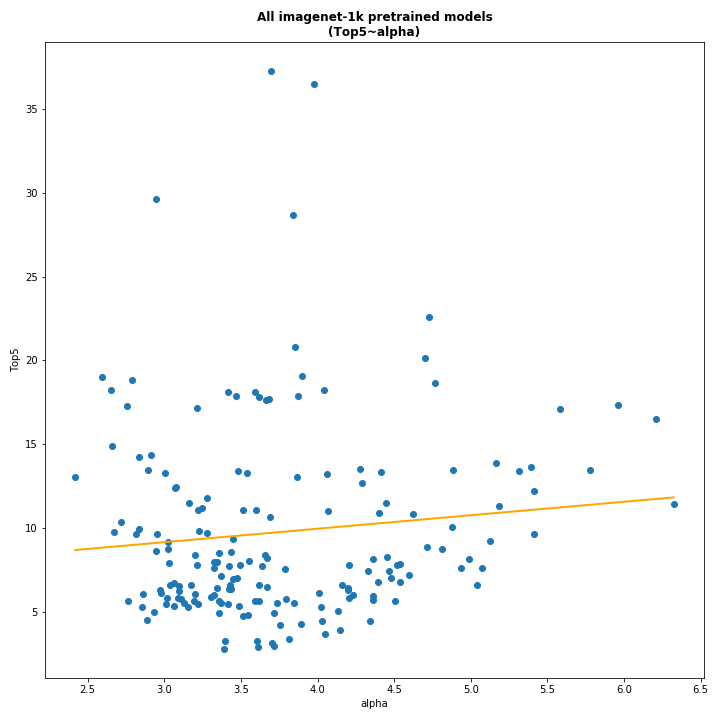
\includegraphics[width=4.9cm]{img/all-imagenet-1k_alpha.png}
%%        \label{fig:imagenet1k-alpha}
%%    }
%%    \qquad
%%    \subfigure[ CIFAR 10 ]{
%%        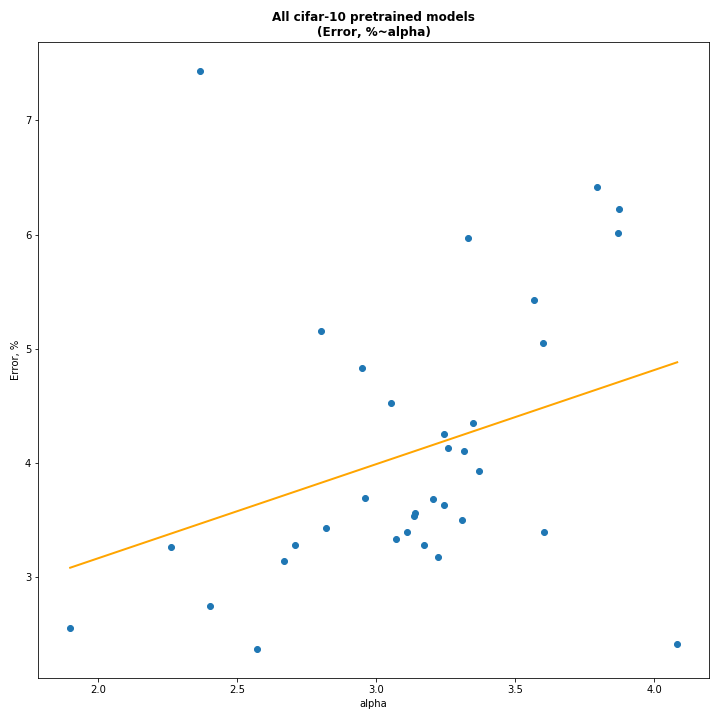
\includegraphics[width=4.9cm]{img/all-cifar-10_alpha.png}
%%        \label{fig:cifar10.alpha}
%%    }
%%    \qquad
%%    \subfigure[ CIFAR 100 ]{
%%        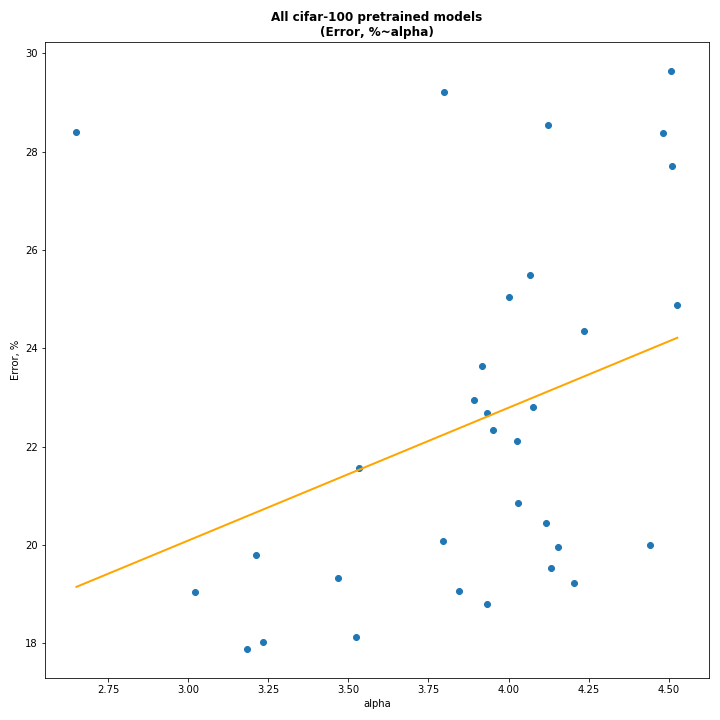
\includegraphics[width=4.9cm]{img/all-cifar-100_alpha.png}
%%        \label{fig:cifar100.alpha}
%%    }
%%    \qquad
%%    \subfigure[ SVHN ]{
%%        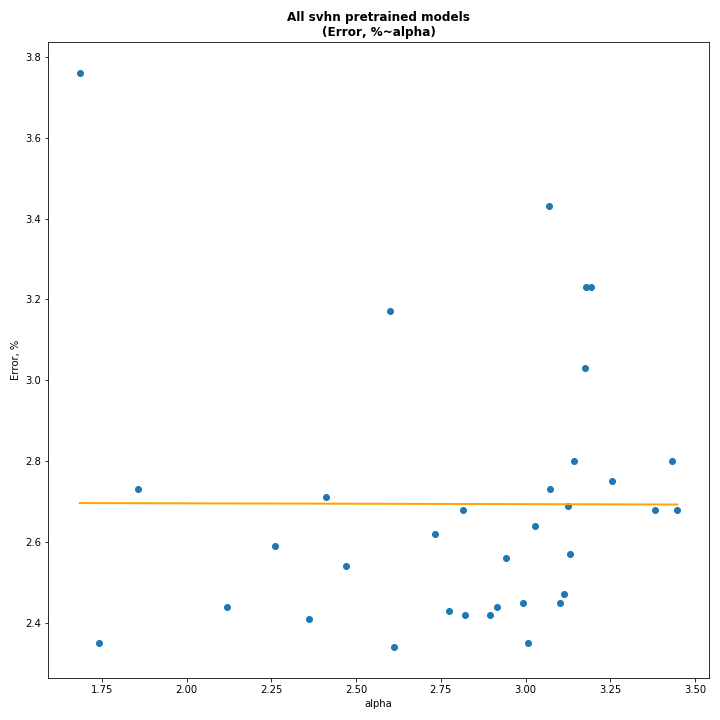
\includegraphics[width=4.9cm]{img/all-svhn_alpha.png}
%%        \label{fig:svhn.alpha}
%%    }
%%    \qquad
%%    \subfigure[ CUB 200 ]{
%%        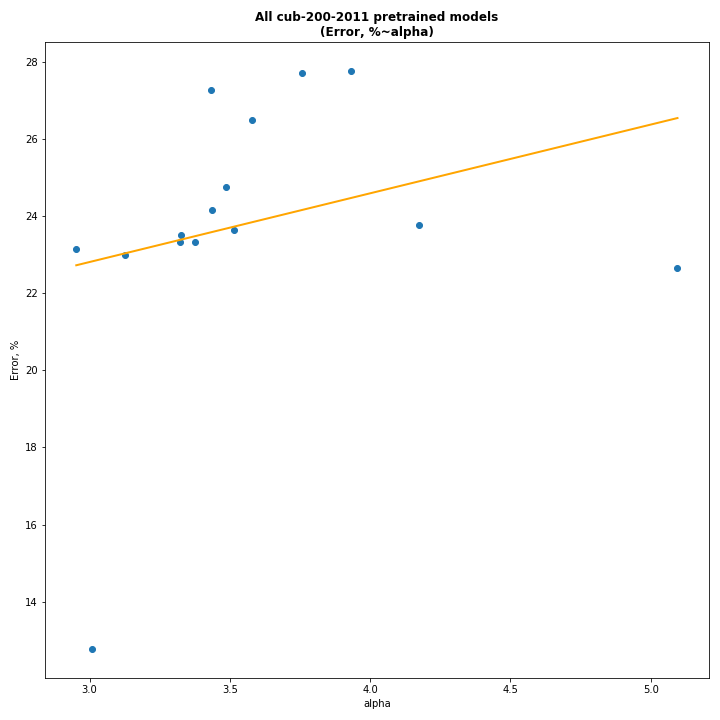
\includegraphics[width=4.9cm]{img/all-cub-200-2011_alpha.png}
%%        \label{fig:cub200.alpha}
%%    }
%%    \caption{PL exponent $\alpha$ versus reported Top1 Test Accuracies for pretrained DNNs available for different datasets (as segmented in Table~\ref{table:datasets}).
%%            }
%%    \label{fig:DSalphas}
%%\end{figure}
%%
%% 
%%\begin{figure}[t]
%%    \centering
%%    \subfigure[ ResNet ]{
%%        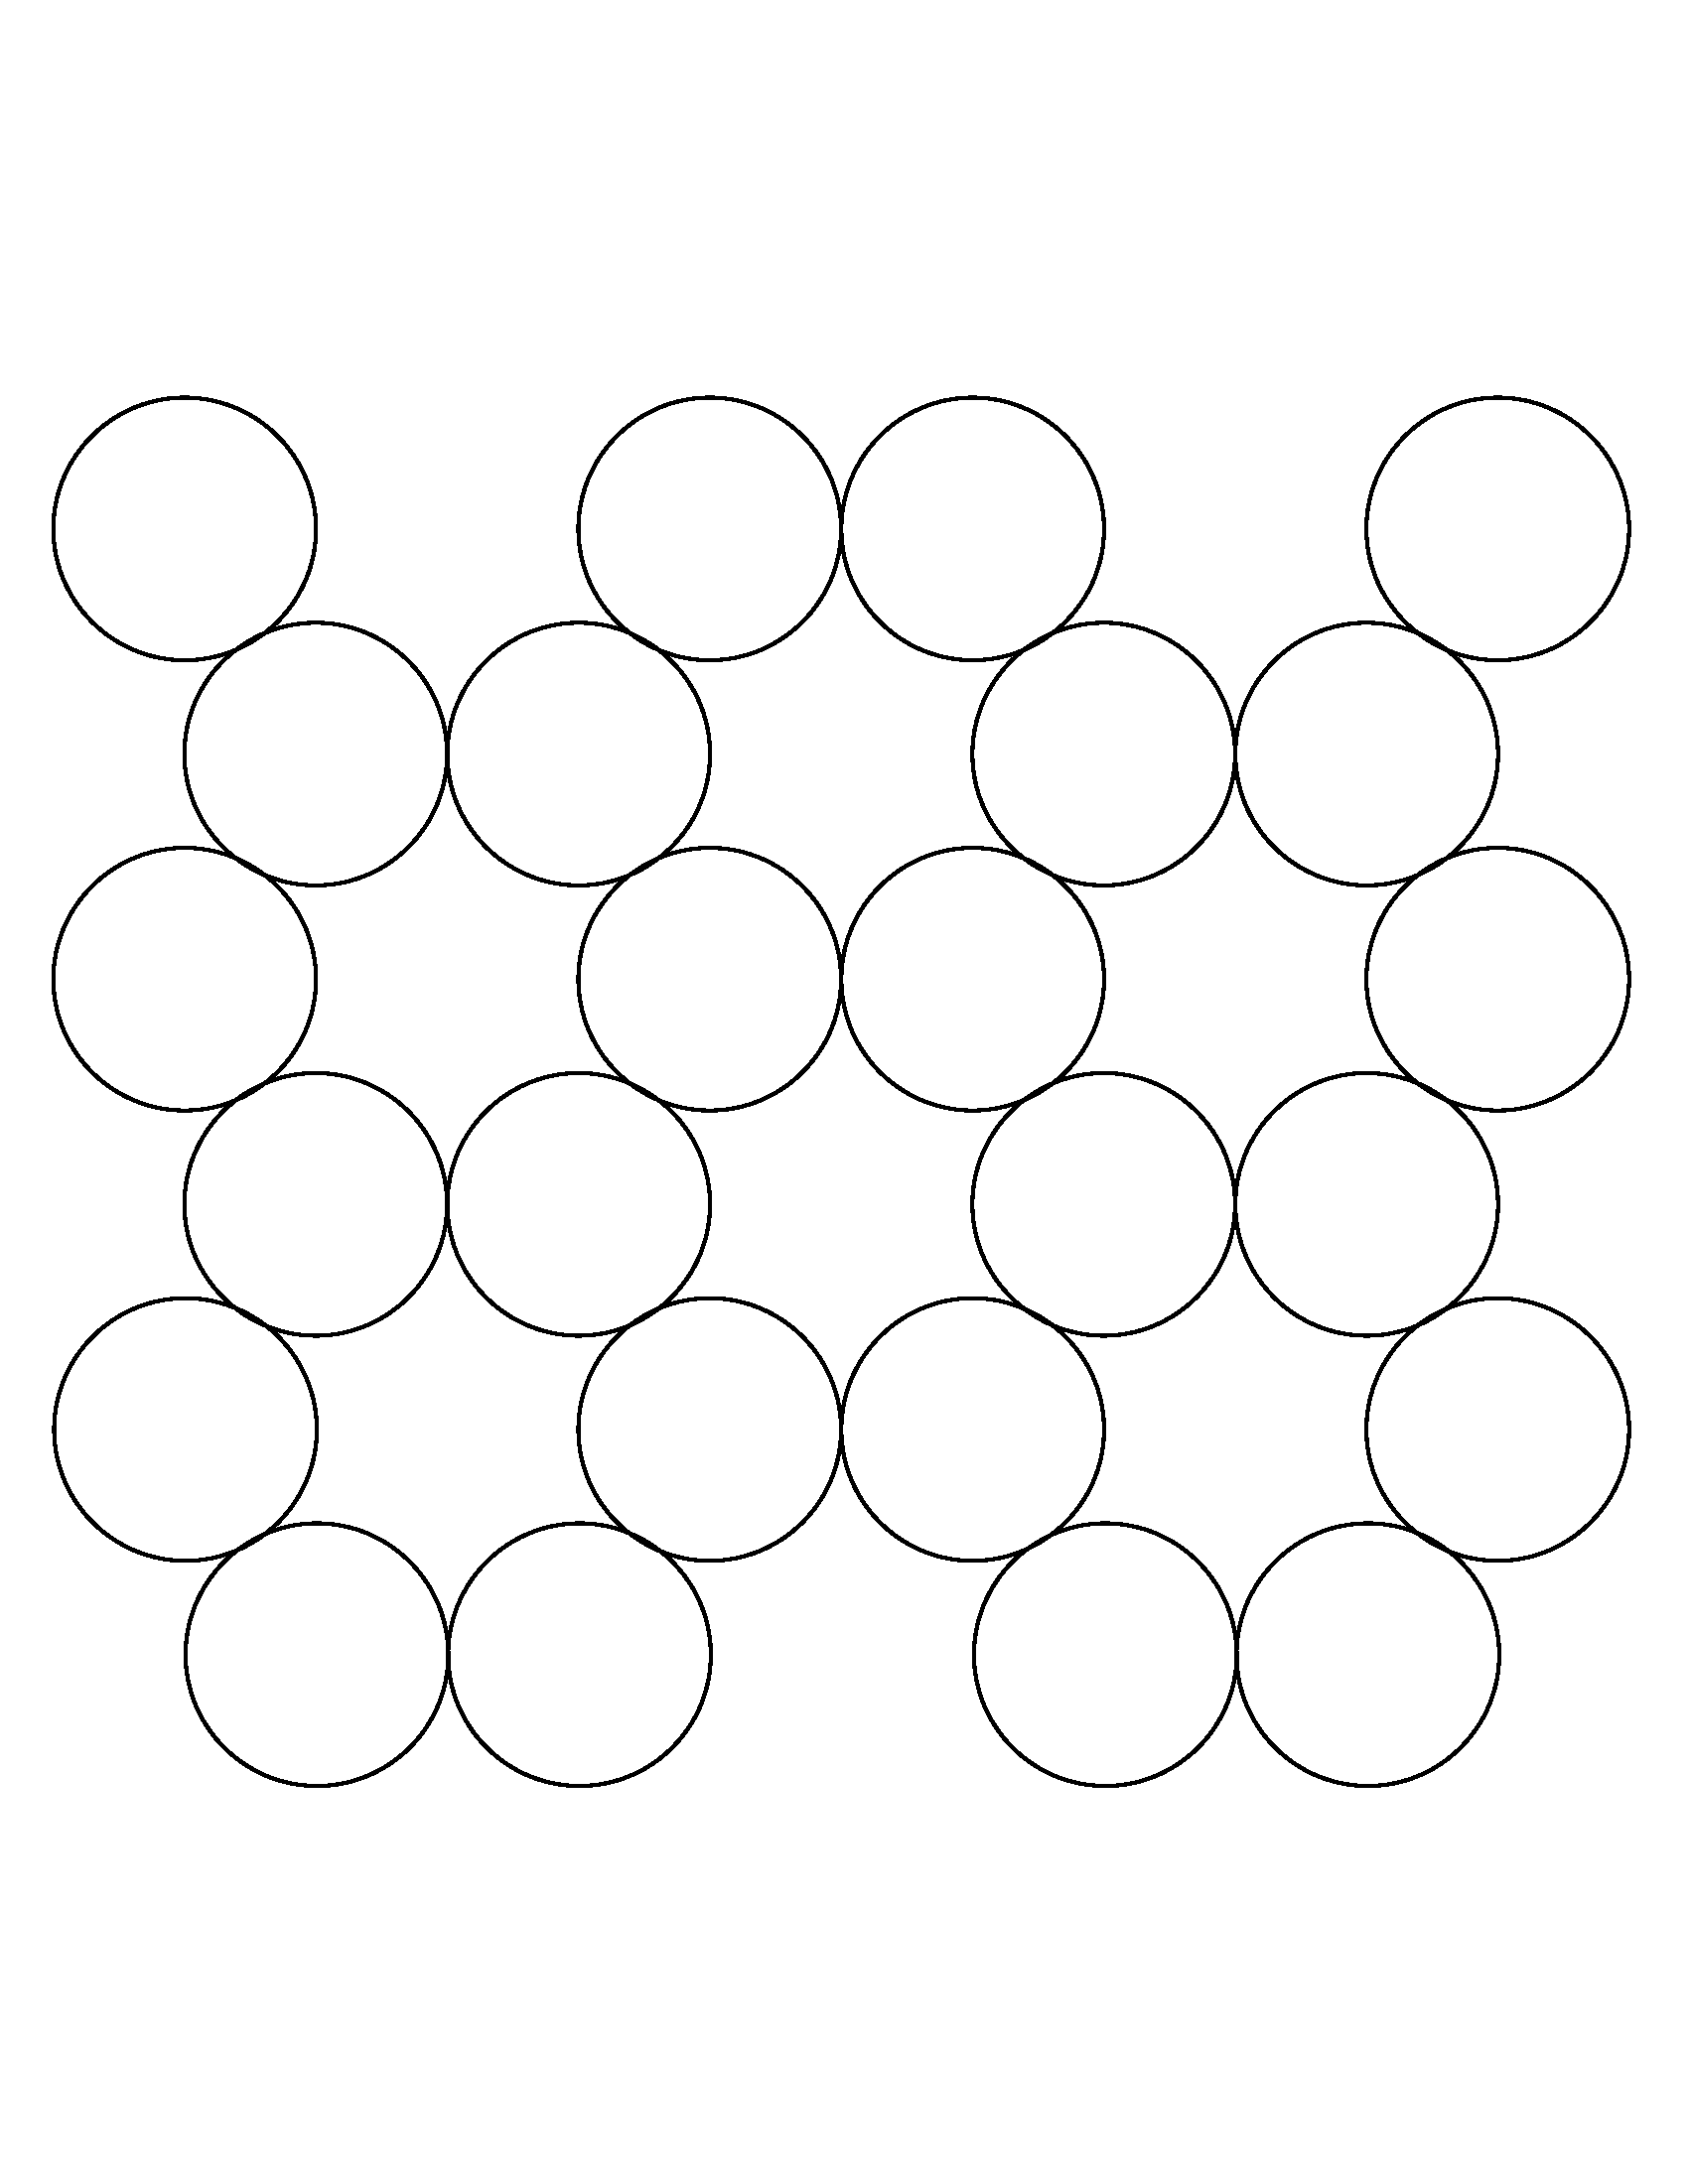
\includegraphics[width=2.7cm]{img/hex.png}
%%        \label{fig:ARCHalphas_01}
%%    }
%%    \subfigure[ SENet/SE-ResNet/SE-PreResNet/SE-ResNeXt ]{
%%        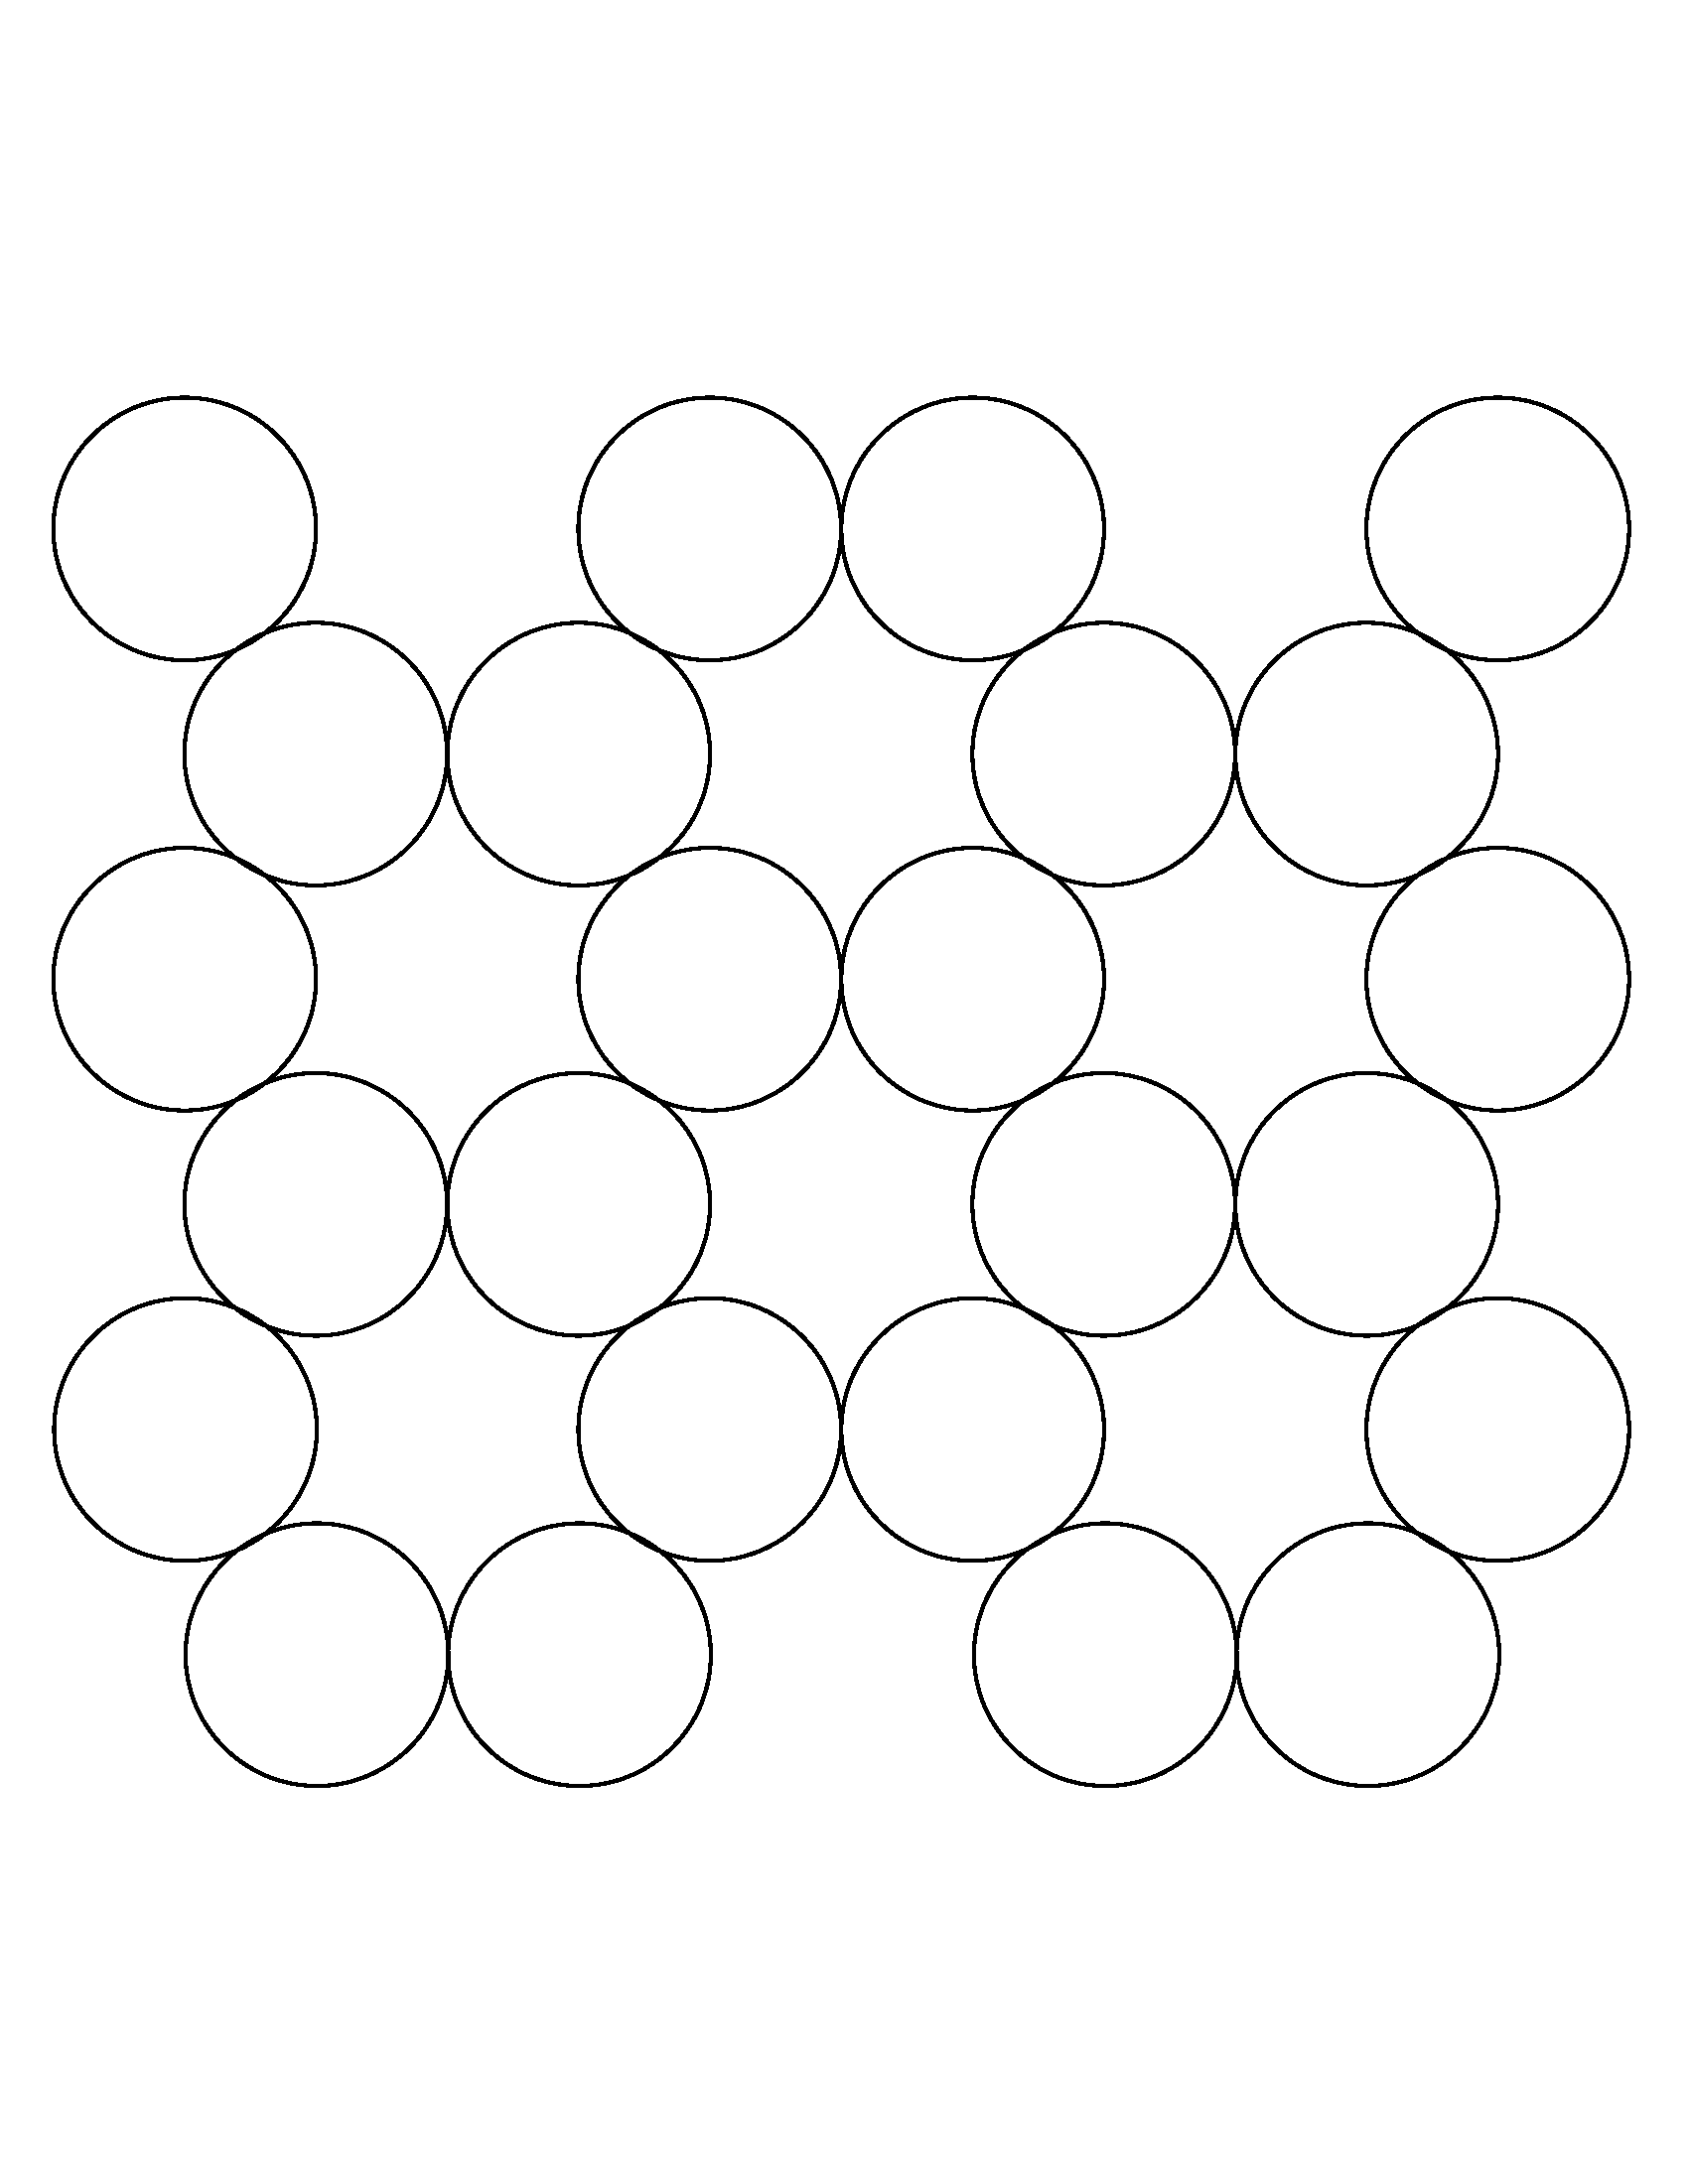
\includegraphics[width=2.7cm]{img/hex.png}
%%        \label{fig:ARCHalphas_02}
%%    }
%%    \subfigure[ DIA-ResNet/DIA-PreResNet ]{
%%        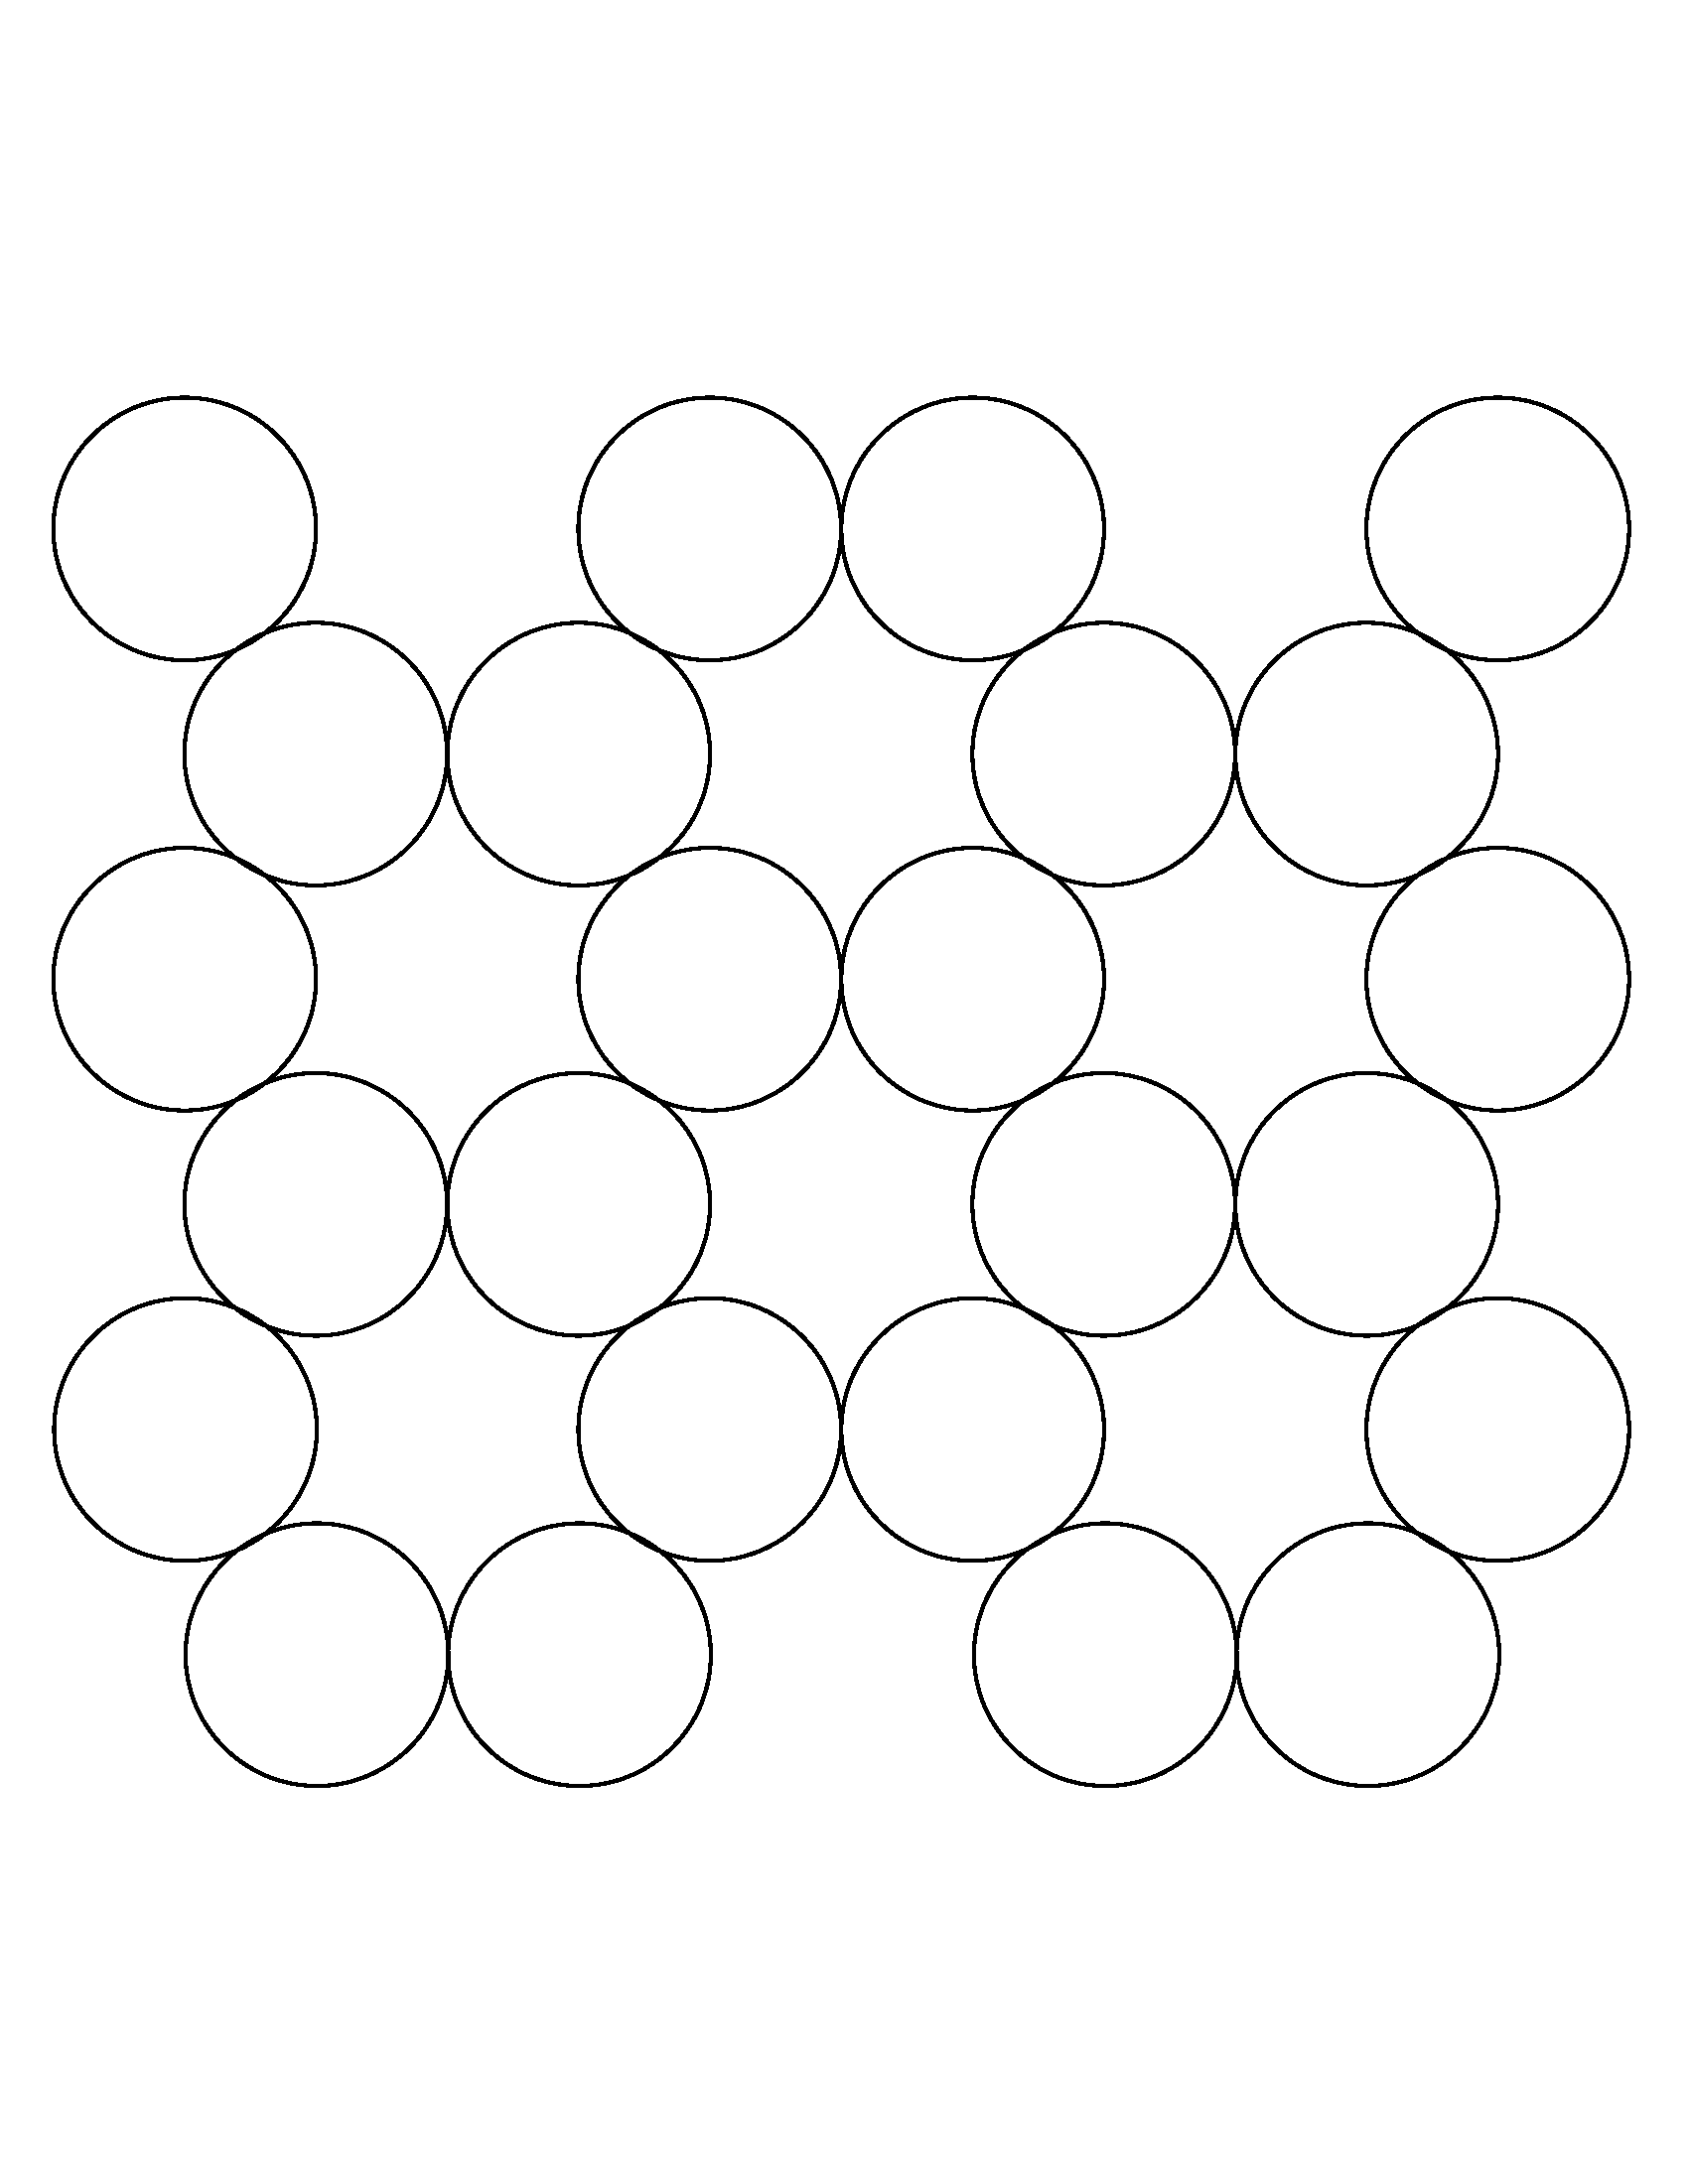
\includegraphics[width=2.7cm]{img/hex.png}
%%        \label{fig:ARCHalphas_03}
%%    }
%%    \subfigure[ ResNeXt ]{
%%        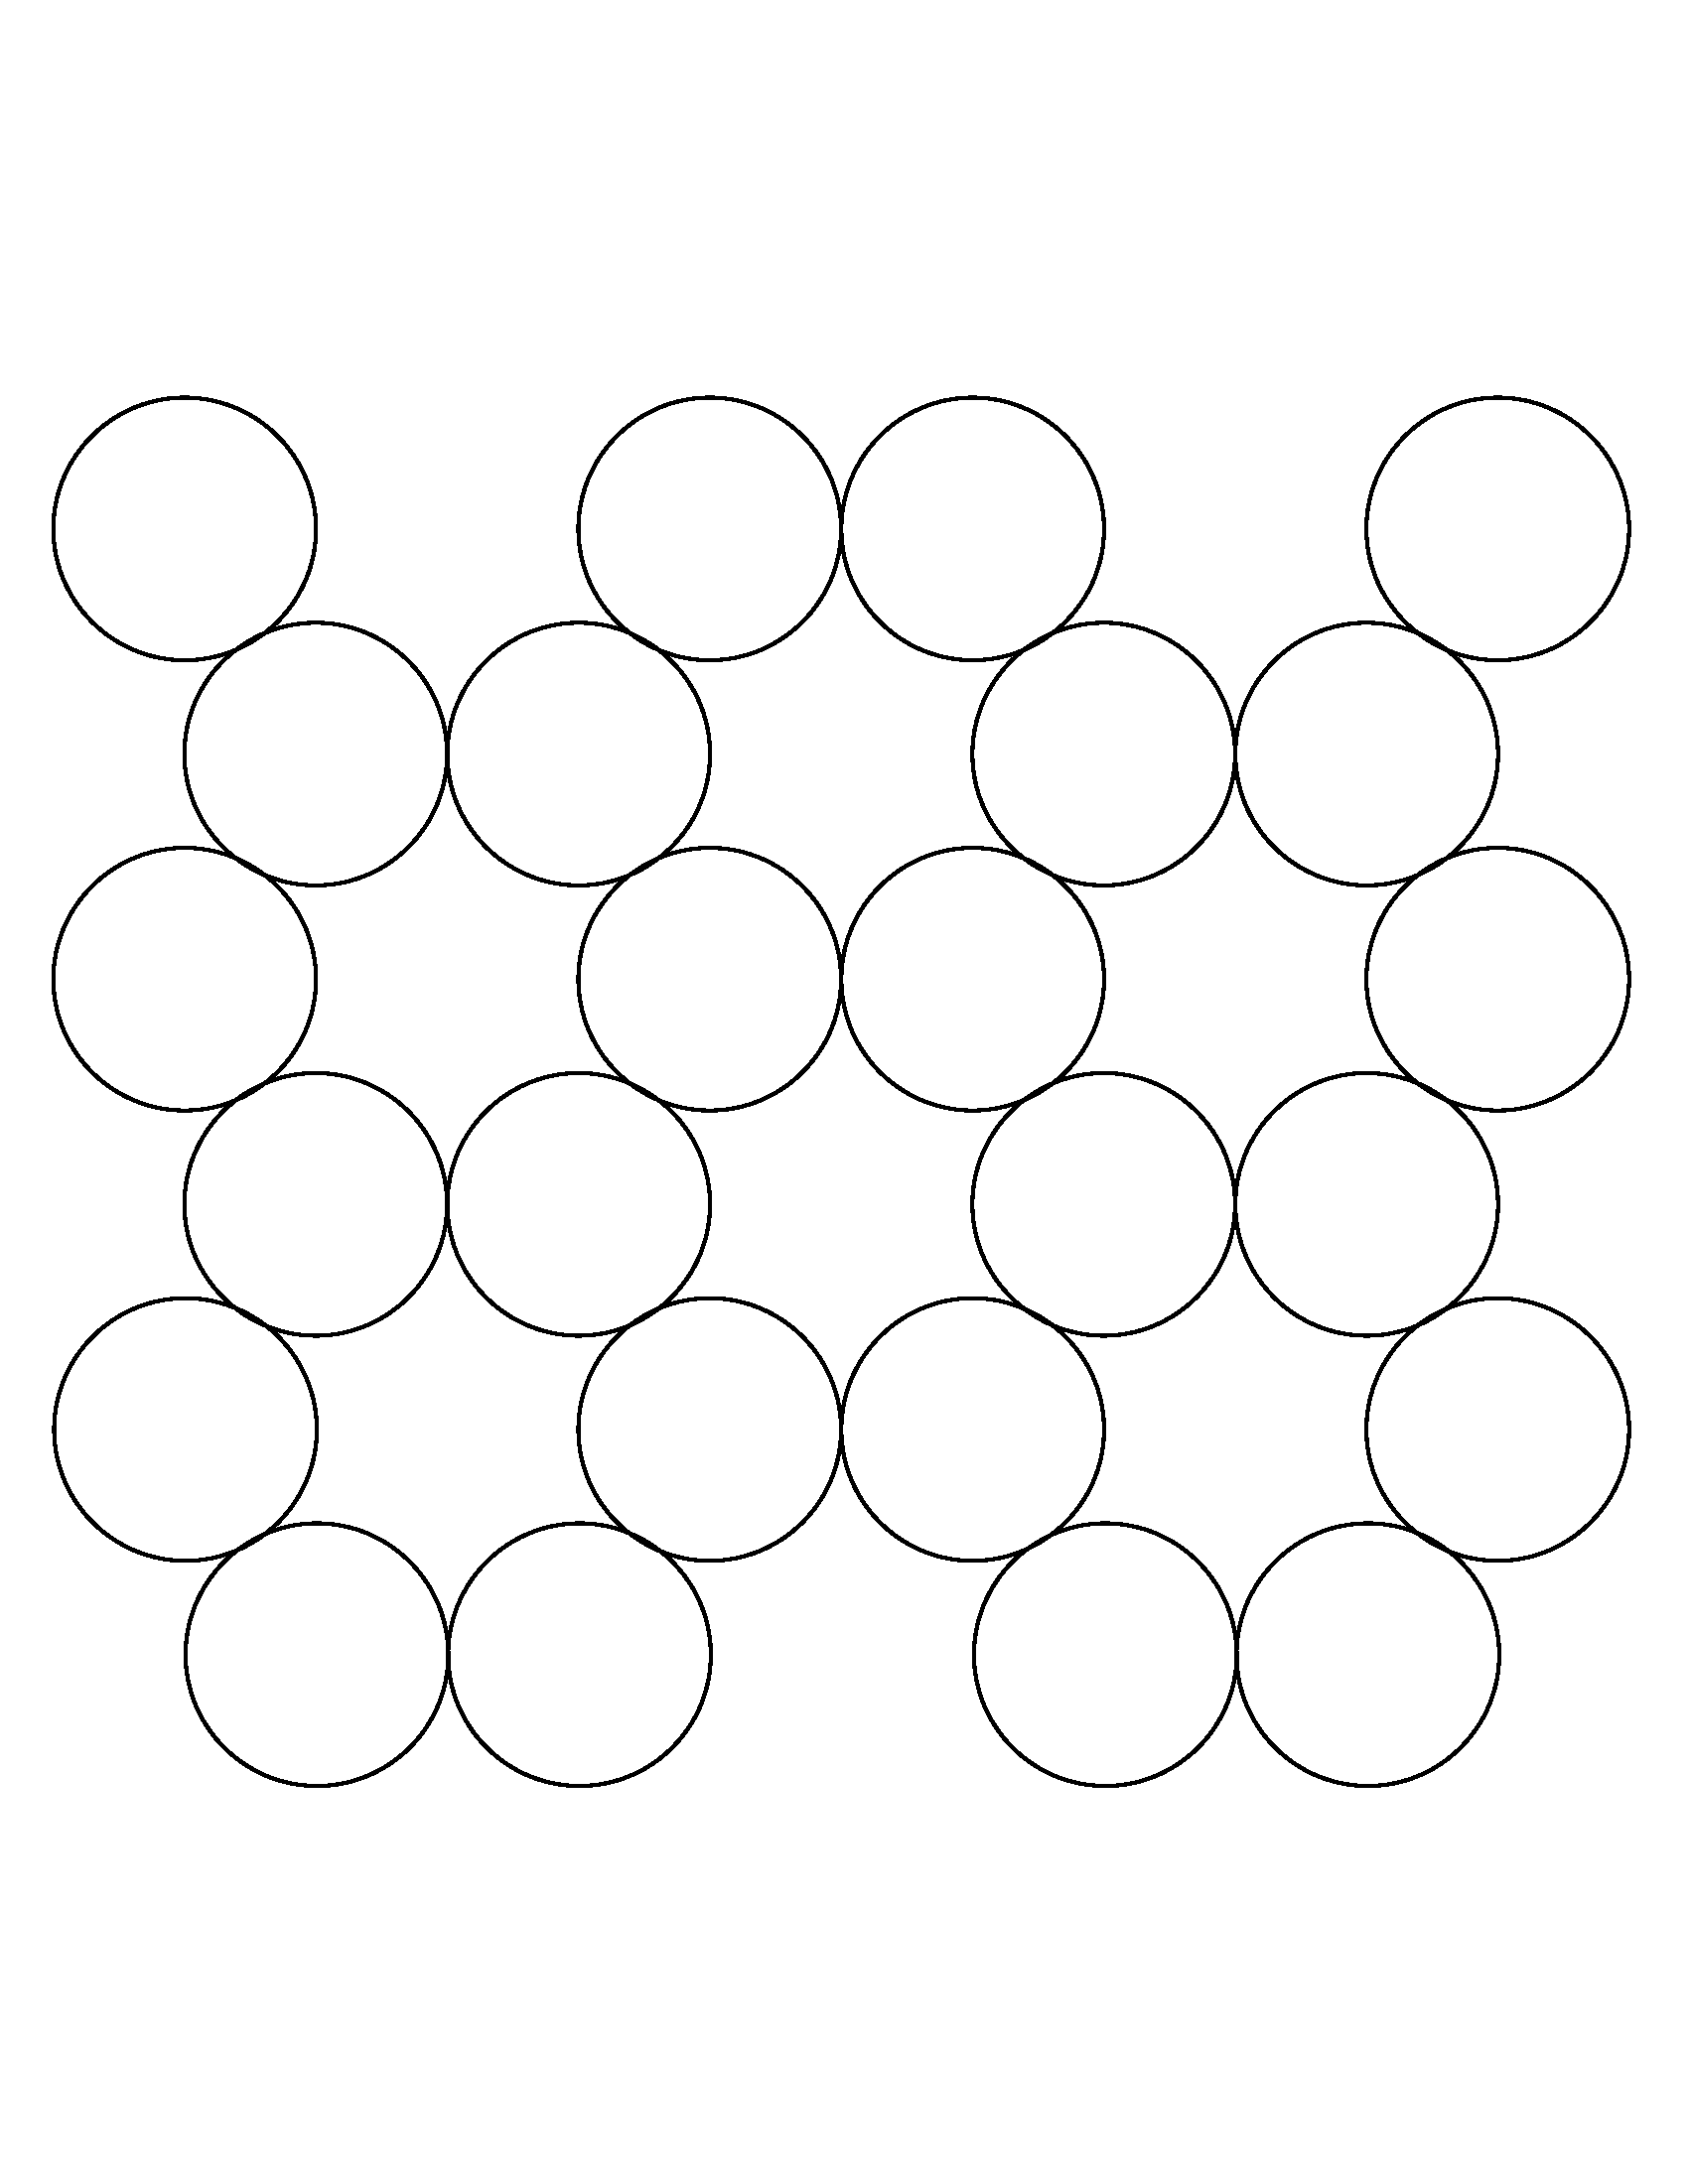
\includegraphics[width=2.7cm]{img/hex.png}
%%        \label{fig:ARCHalphas_04}
%%    }
%%    \subfigure[ WRN ]{
%%        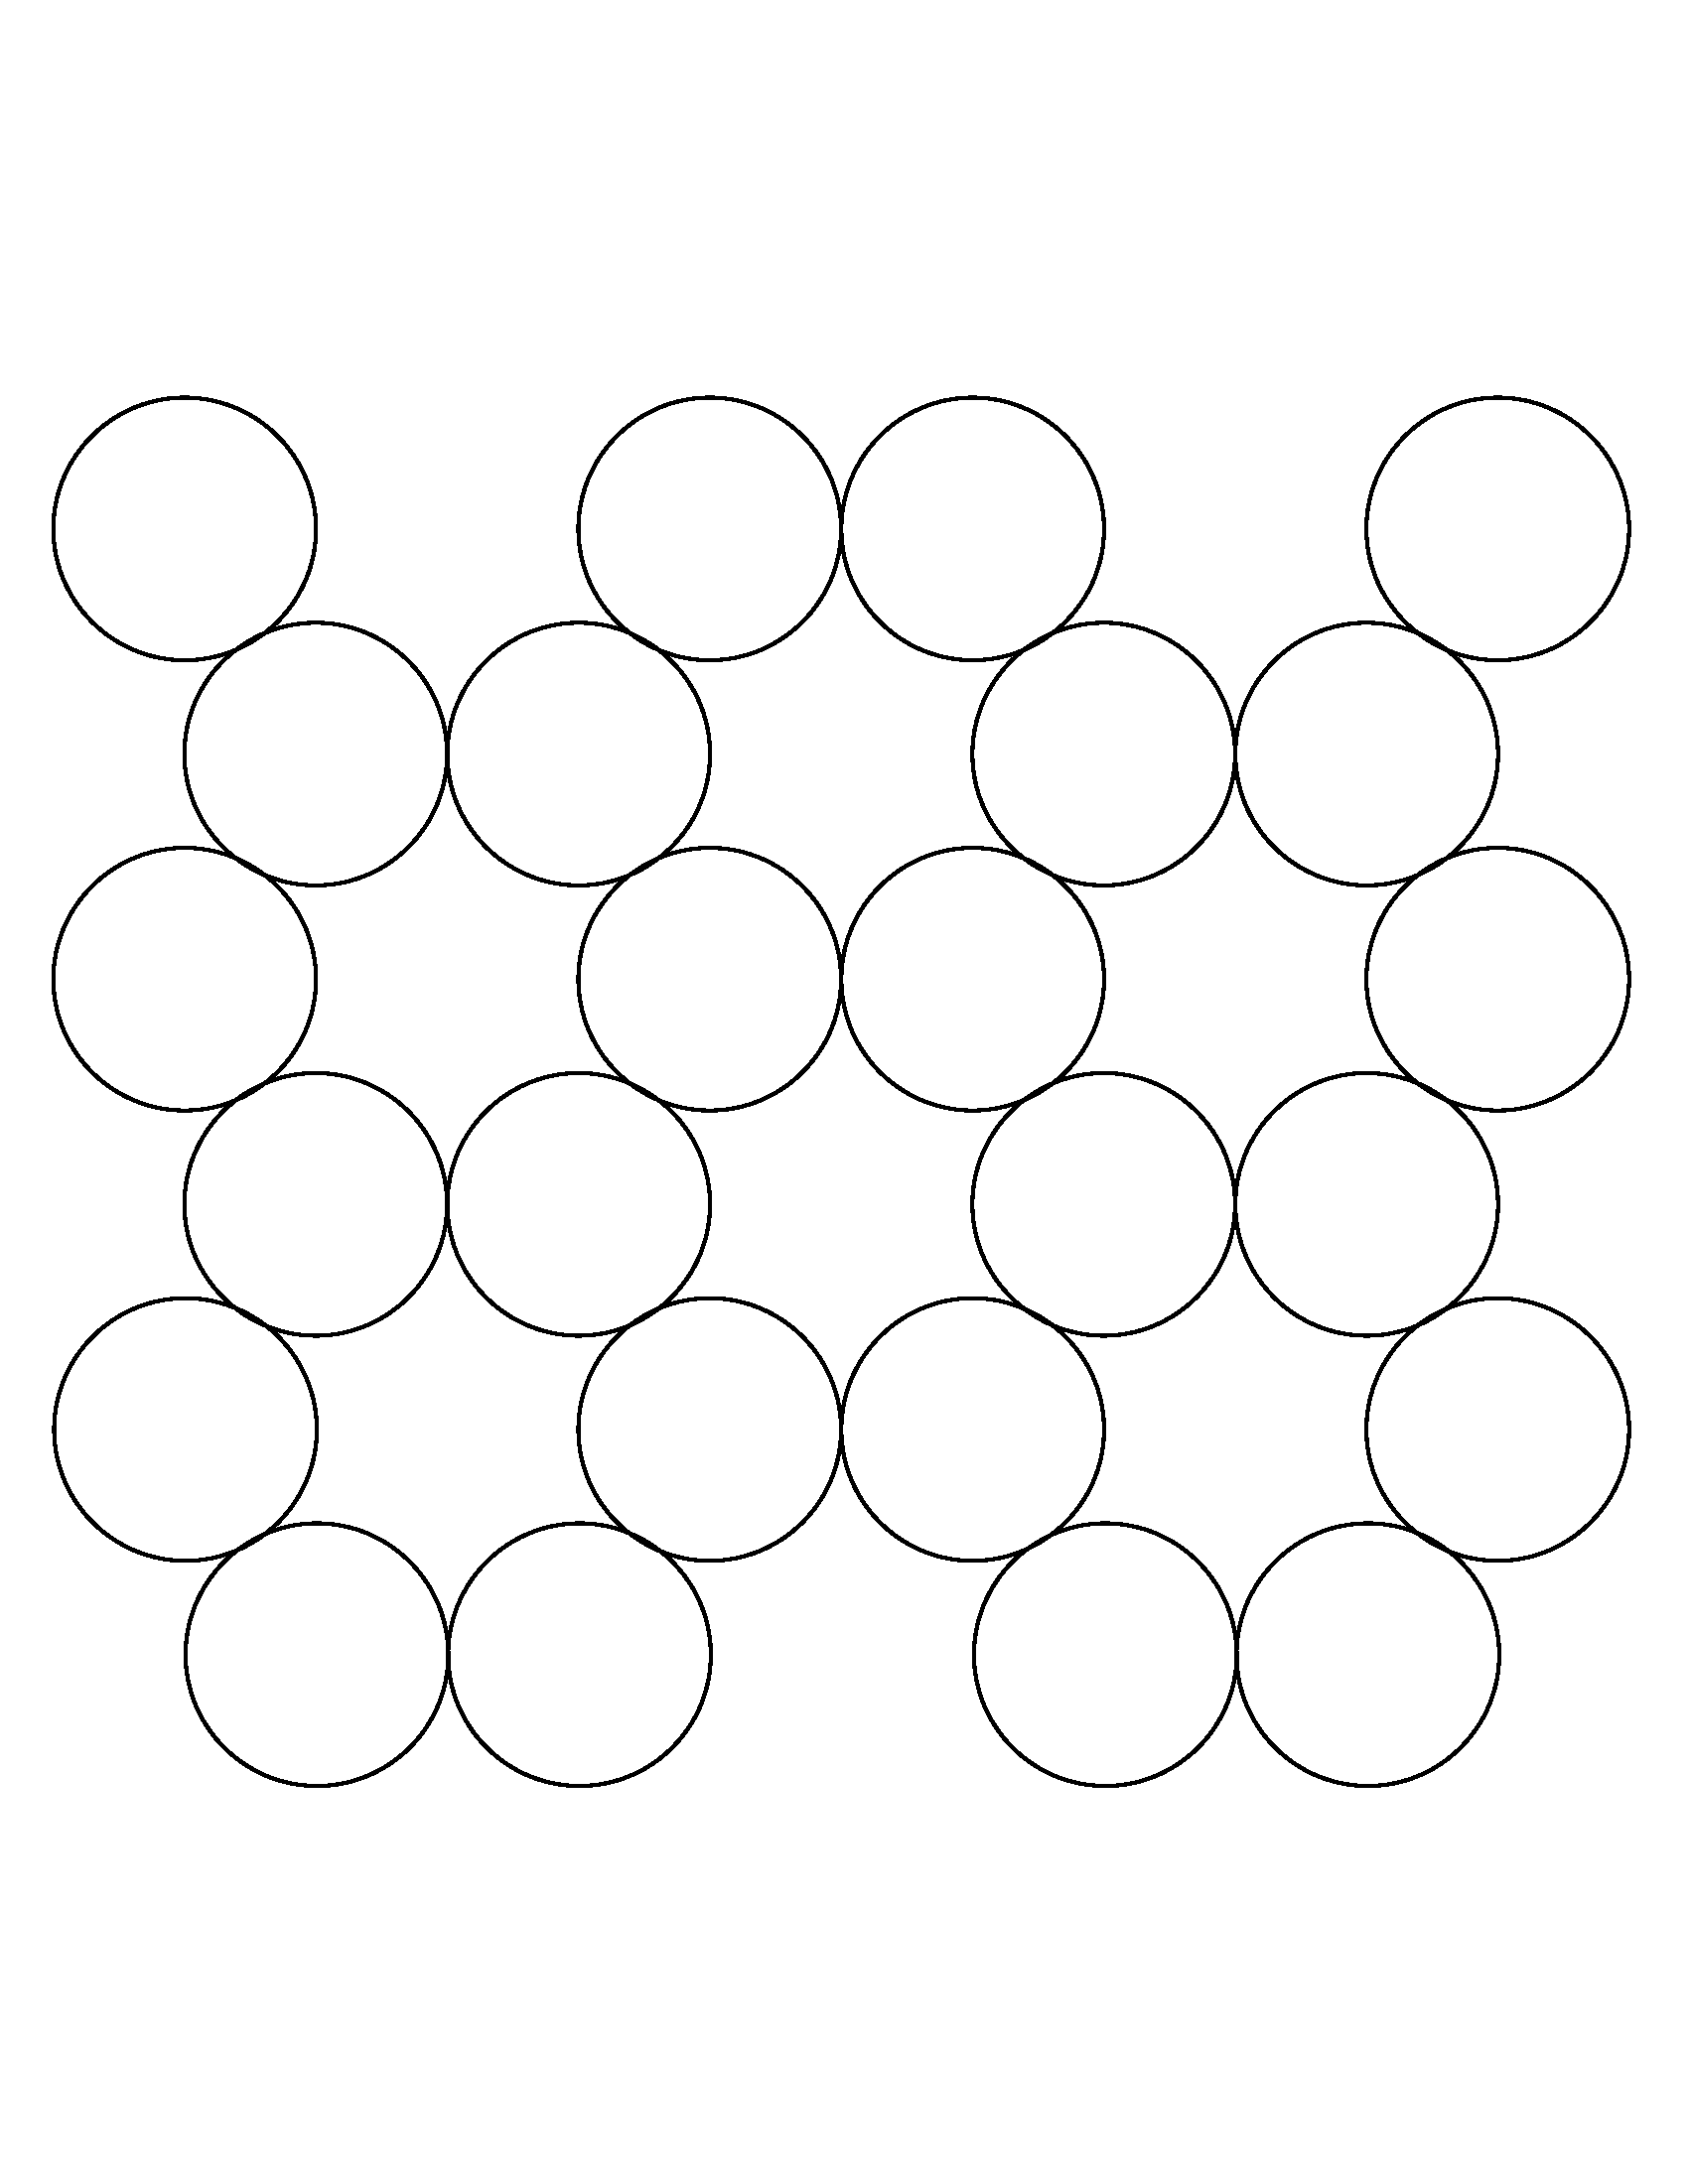
\includegraphics[width=2.7cm]{img/hex.png}
%%        \label{fig:ARCHalphas_05}
%%    }
%%    \subfigure[ DLA ]{
%%        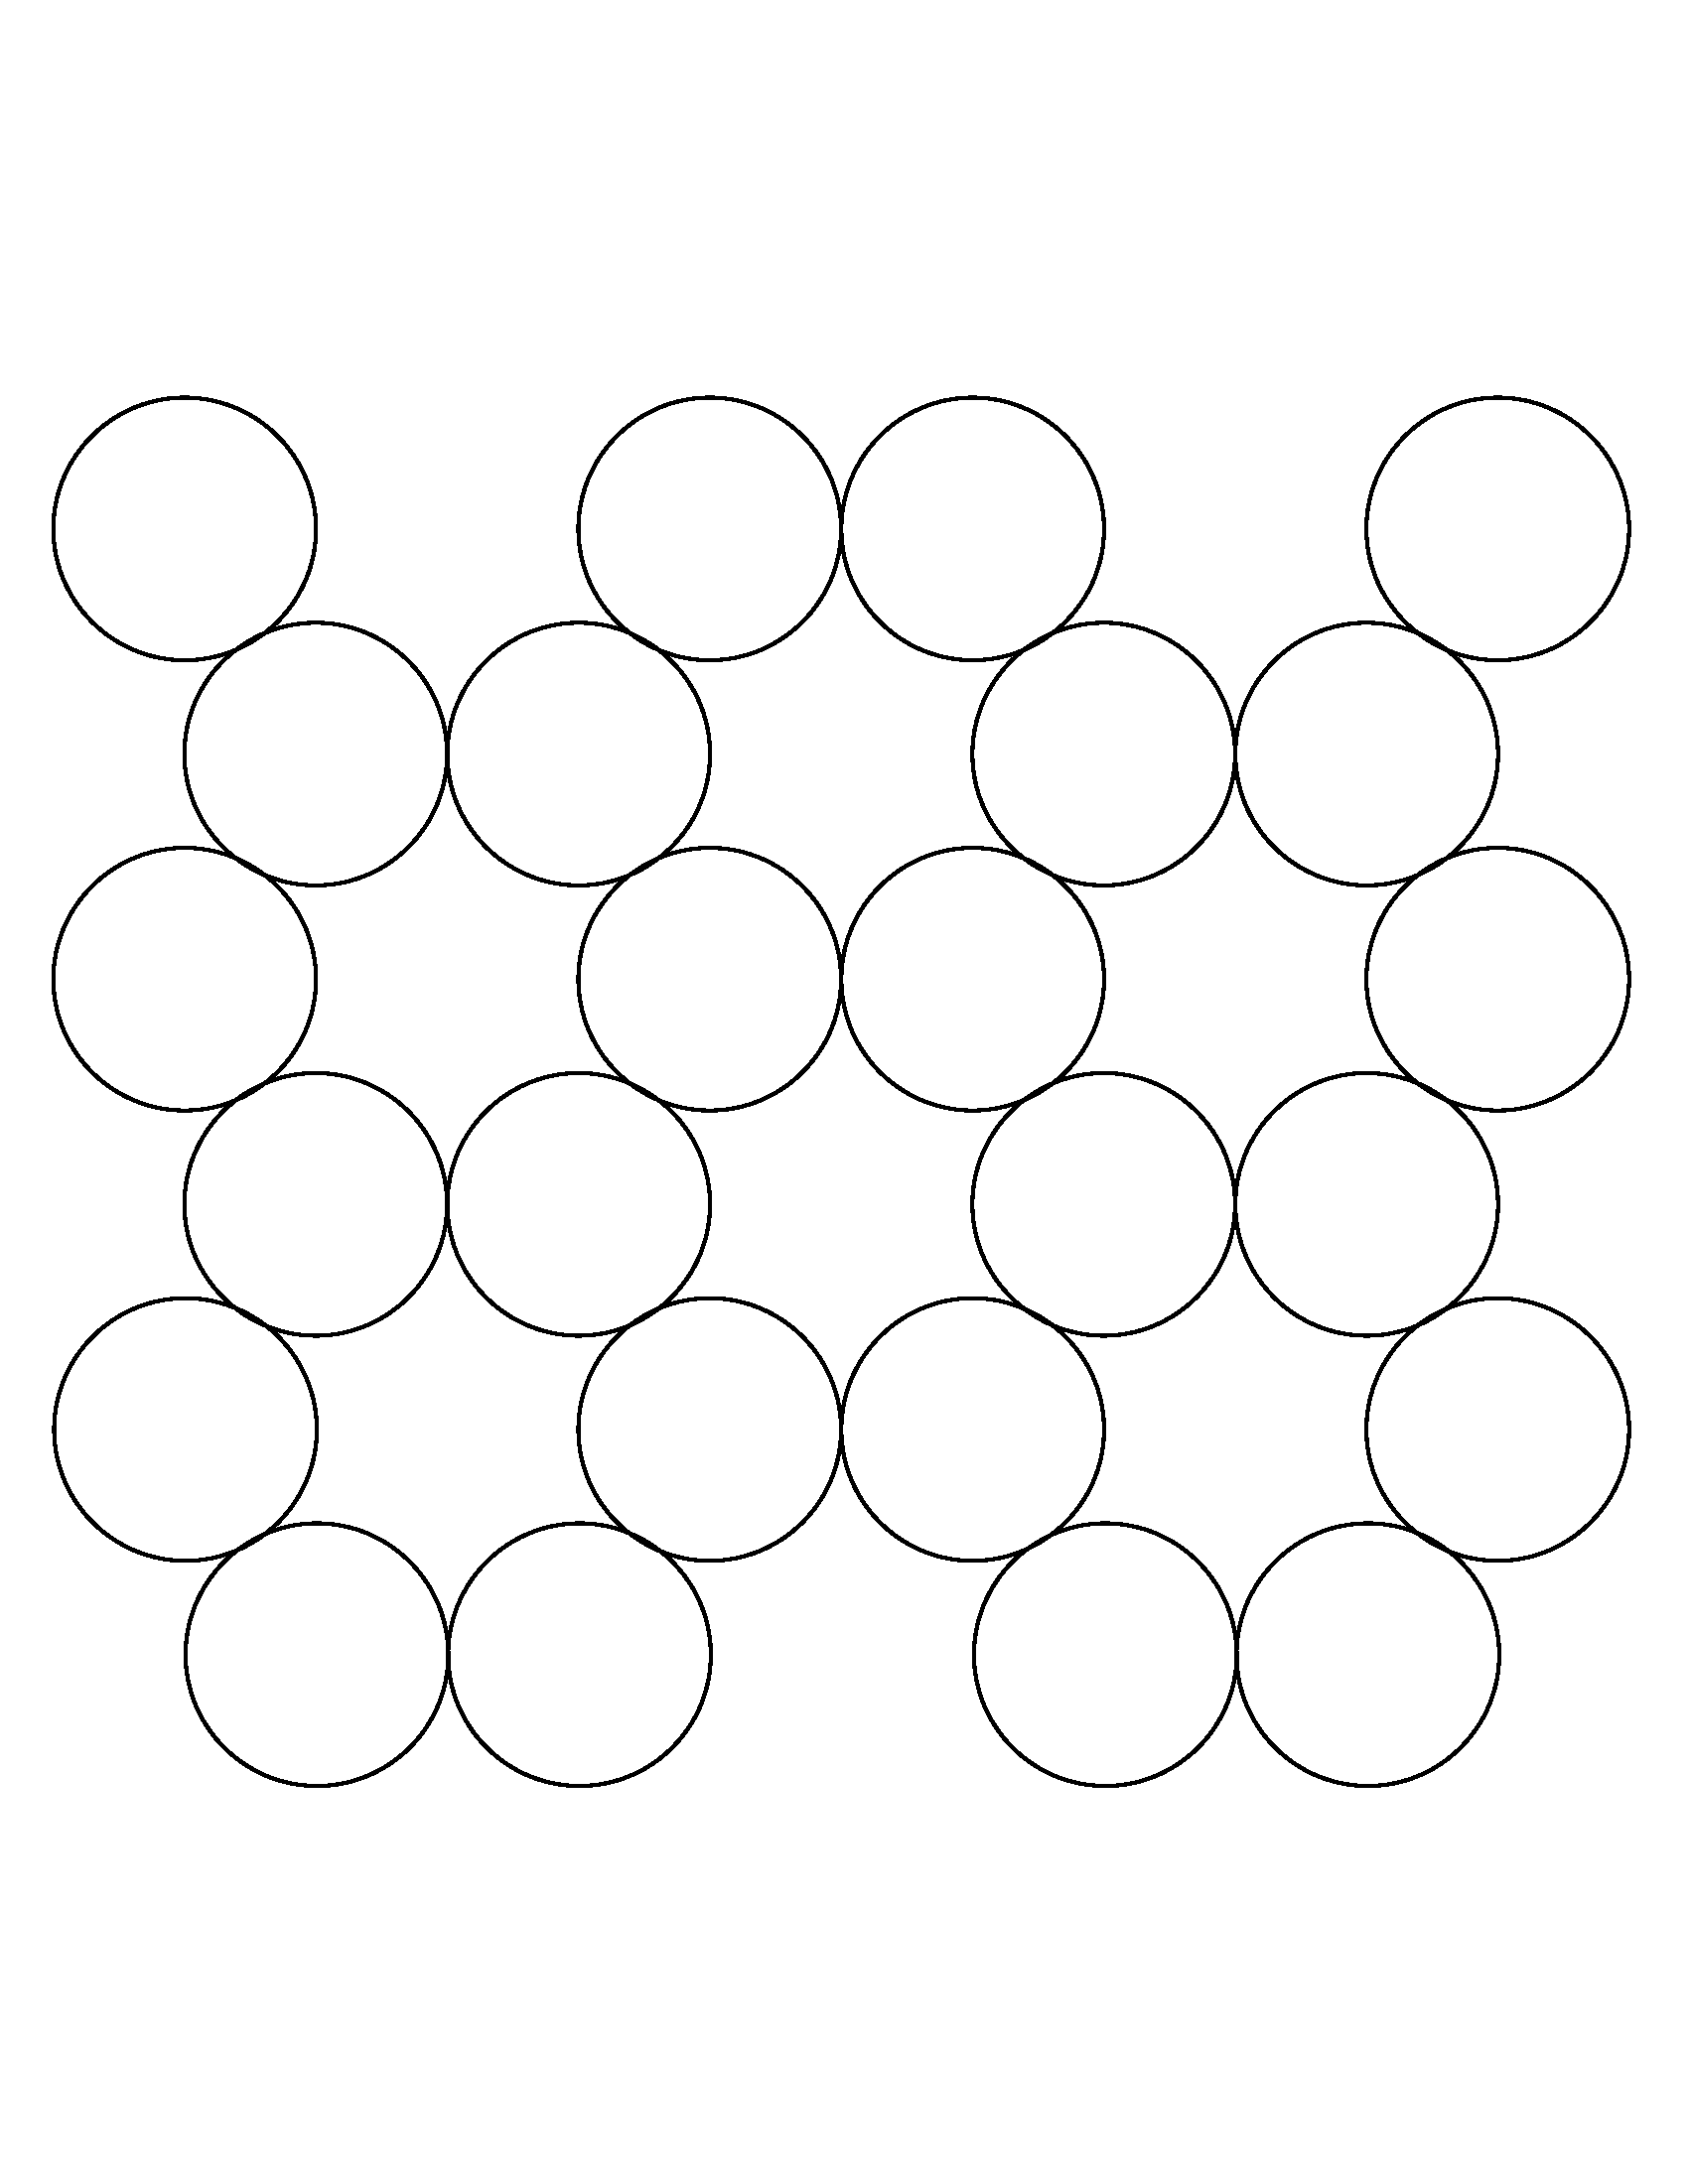
\includegraphics[width=2.7cm]{img/hex.png}
%%        \label{fig:ARCHalphas_06}
%%    }
%%    \subfigure[ PreResNet ]{
%%        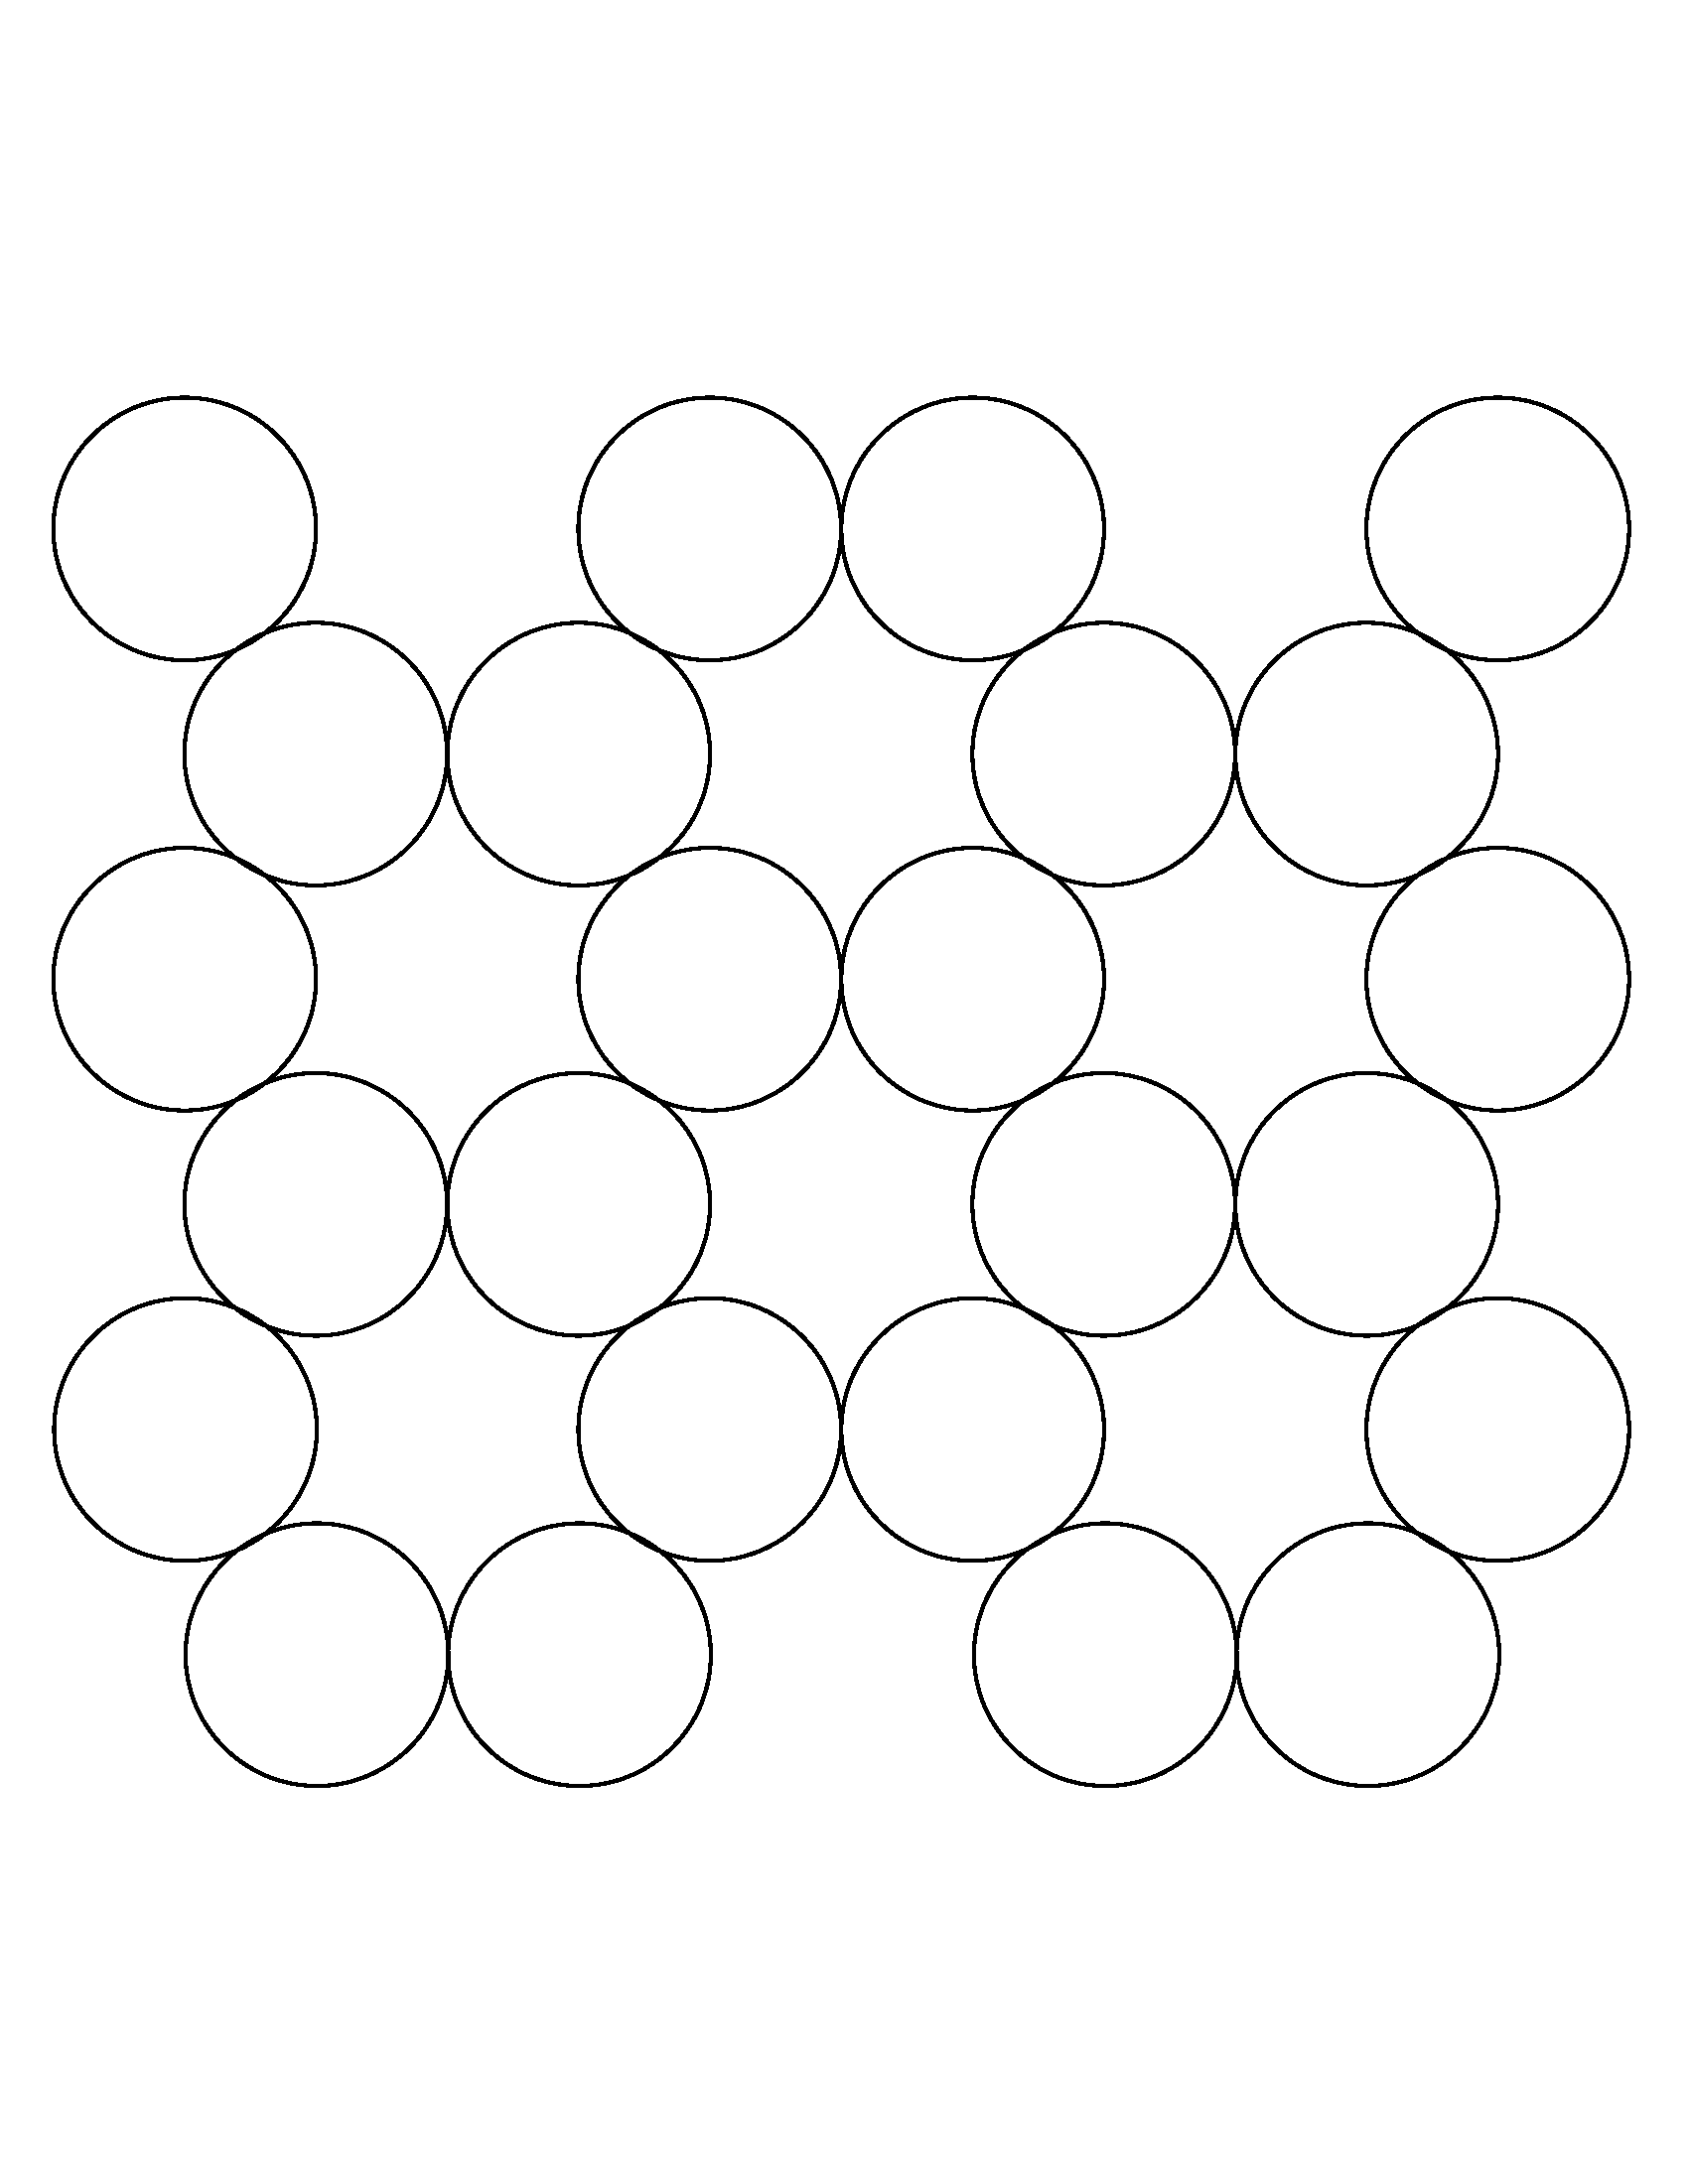
\includegraphics[width=2.7cm]{img/hex.png}
%%        \label{fig:ARCHalphas_07}
%%    }
%%    \subfigure[ ProxylessNAS ]{
%%        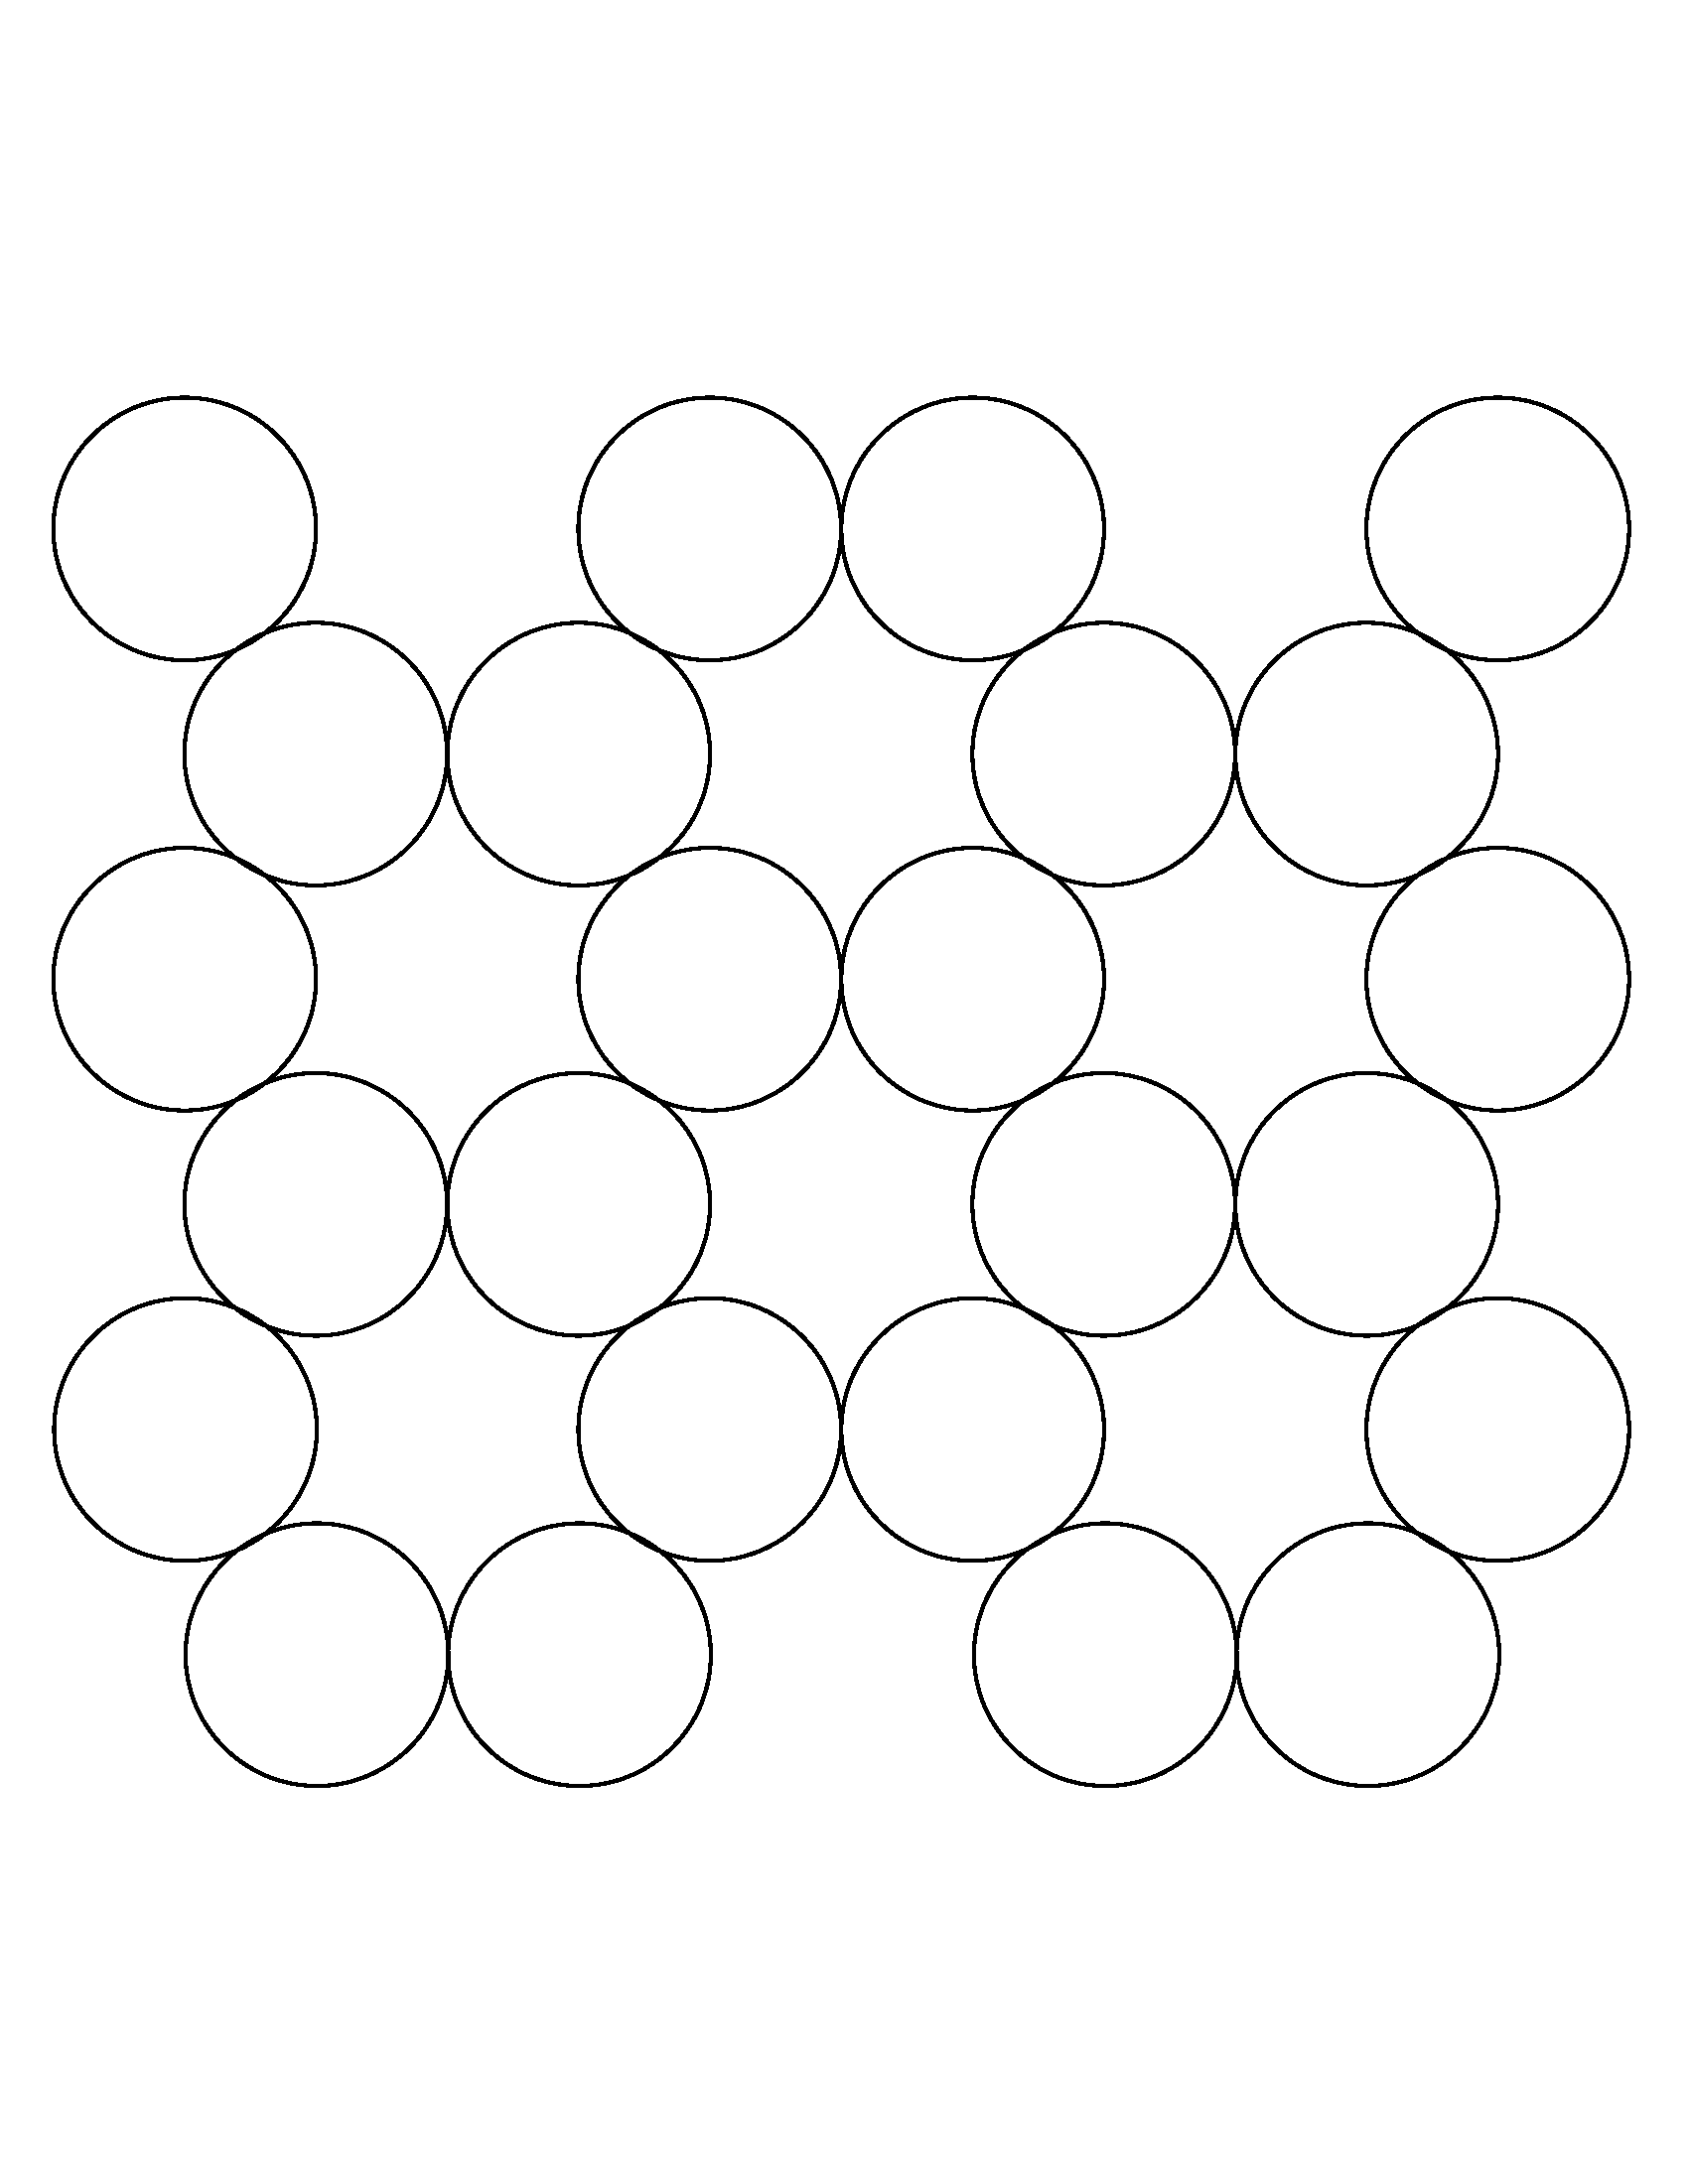
\includegraphics[width=2.7cm]{img/hex.png}
%%        \label{fig:ARCHalphas_08}
%%    }
%%    \subfigure[ VGG/BN-VGG ]{
%%        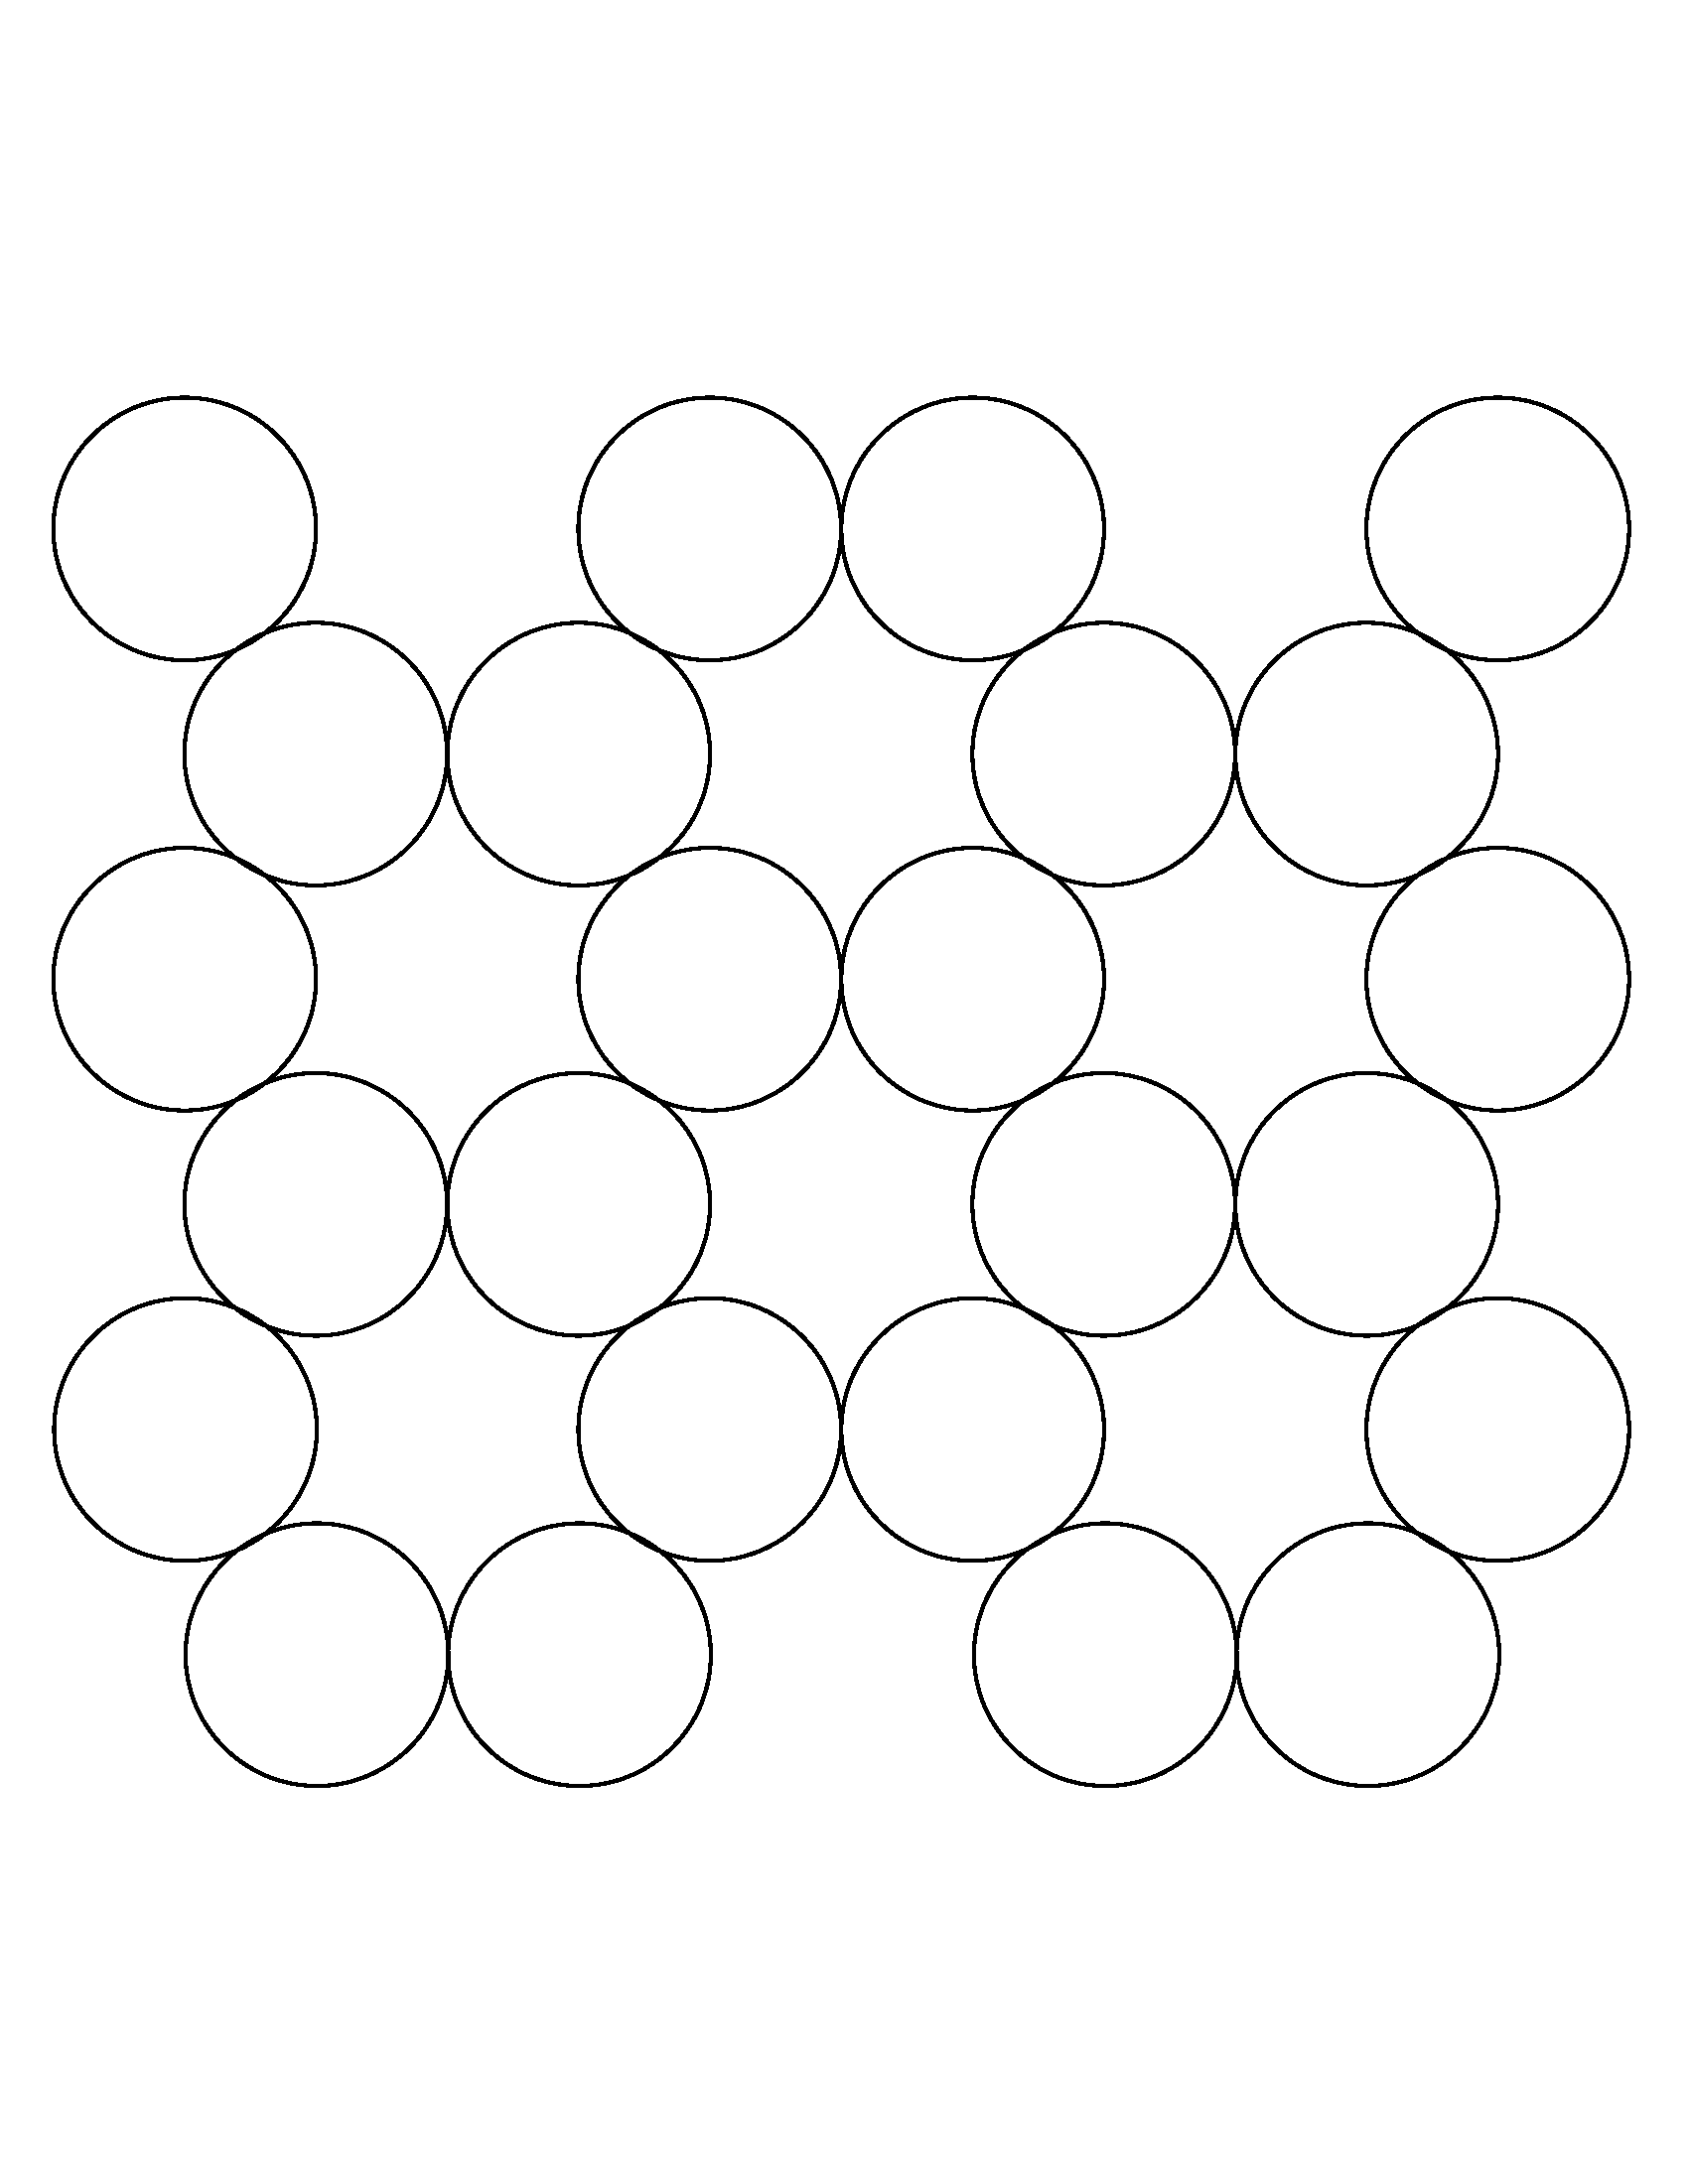
\includegraphics[width=2.7cm]{img/hex.png}
%%        \label{fig:ARCHalphas_09}
%%    }
%%    \subfigure[ IGCV3 ]{
%%        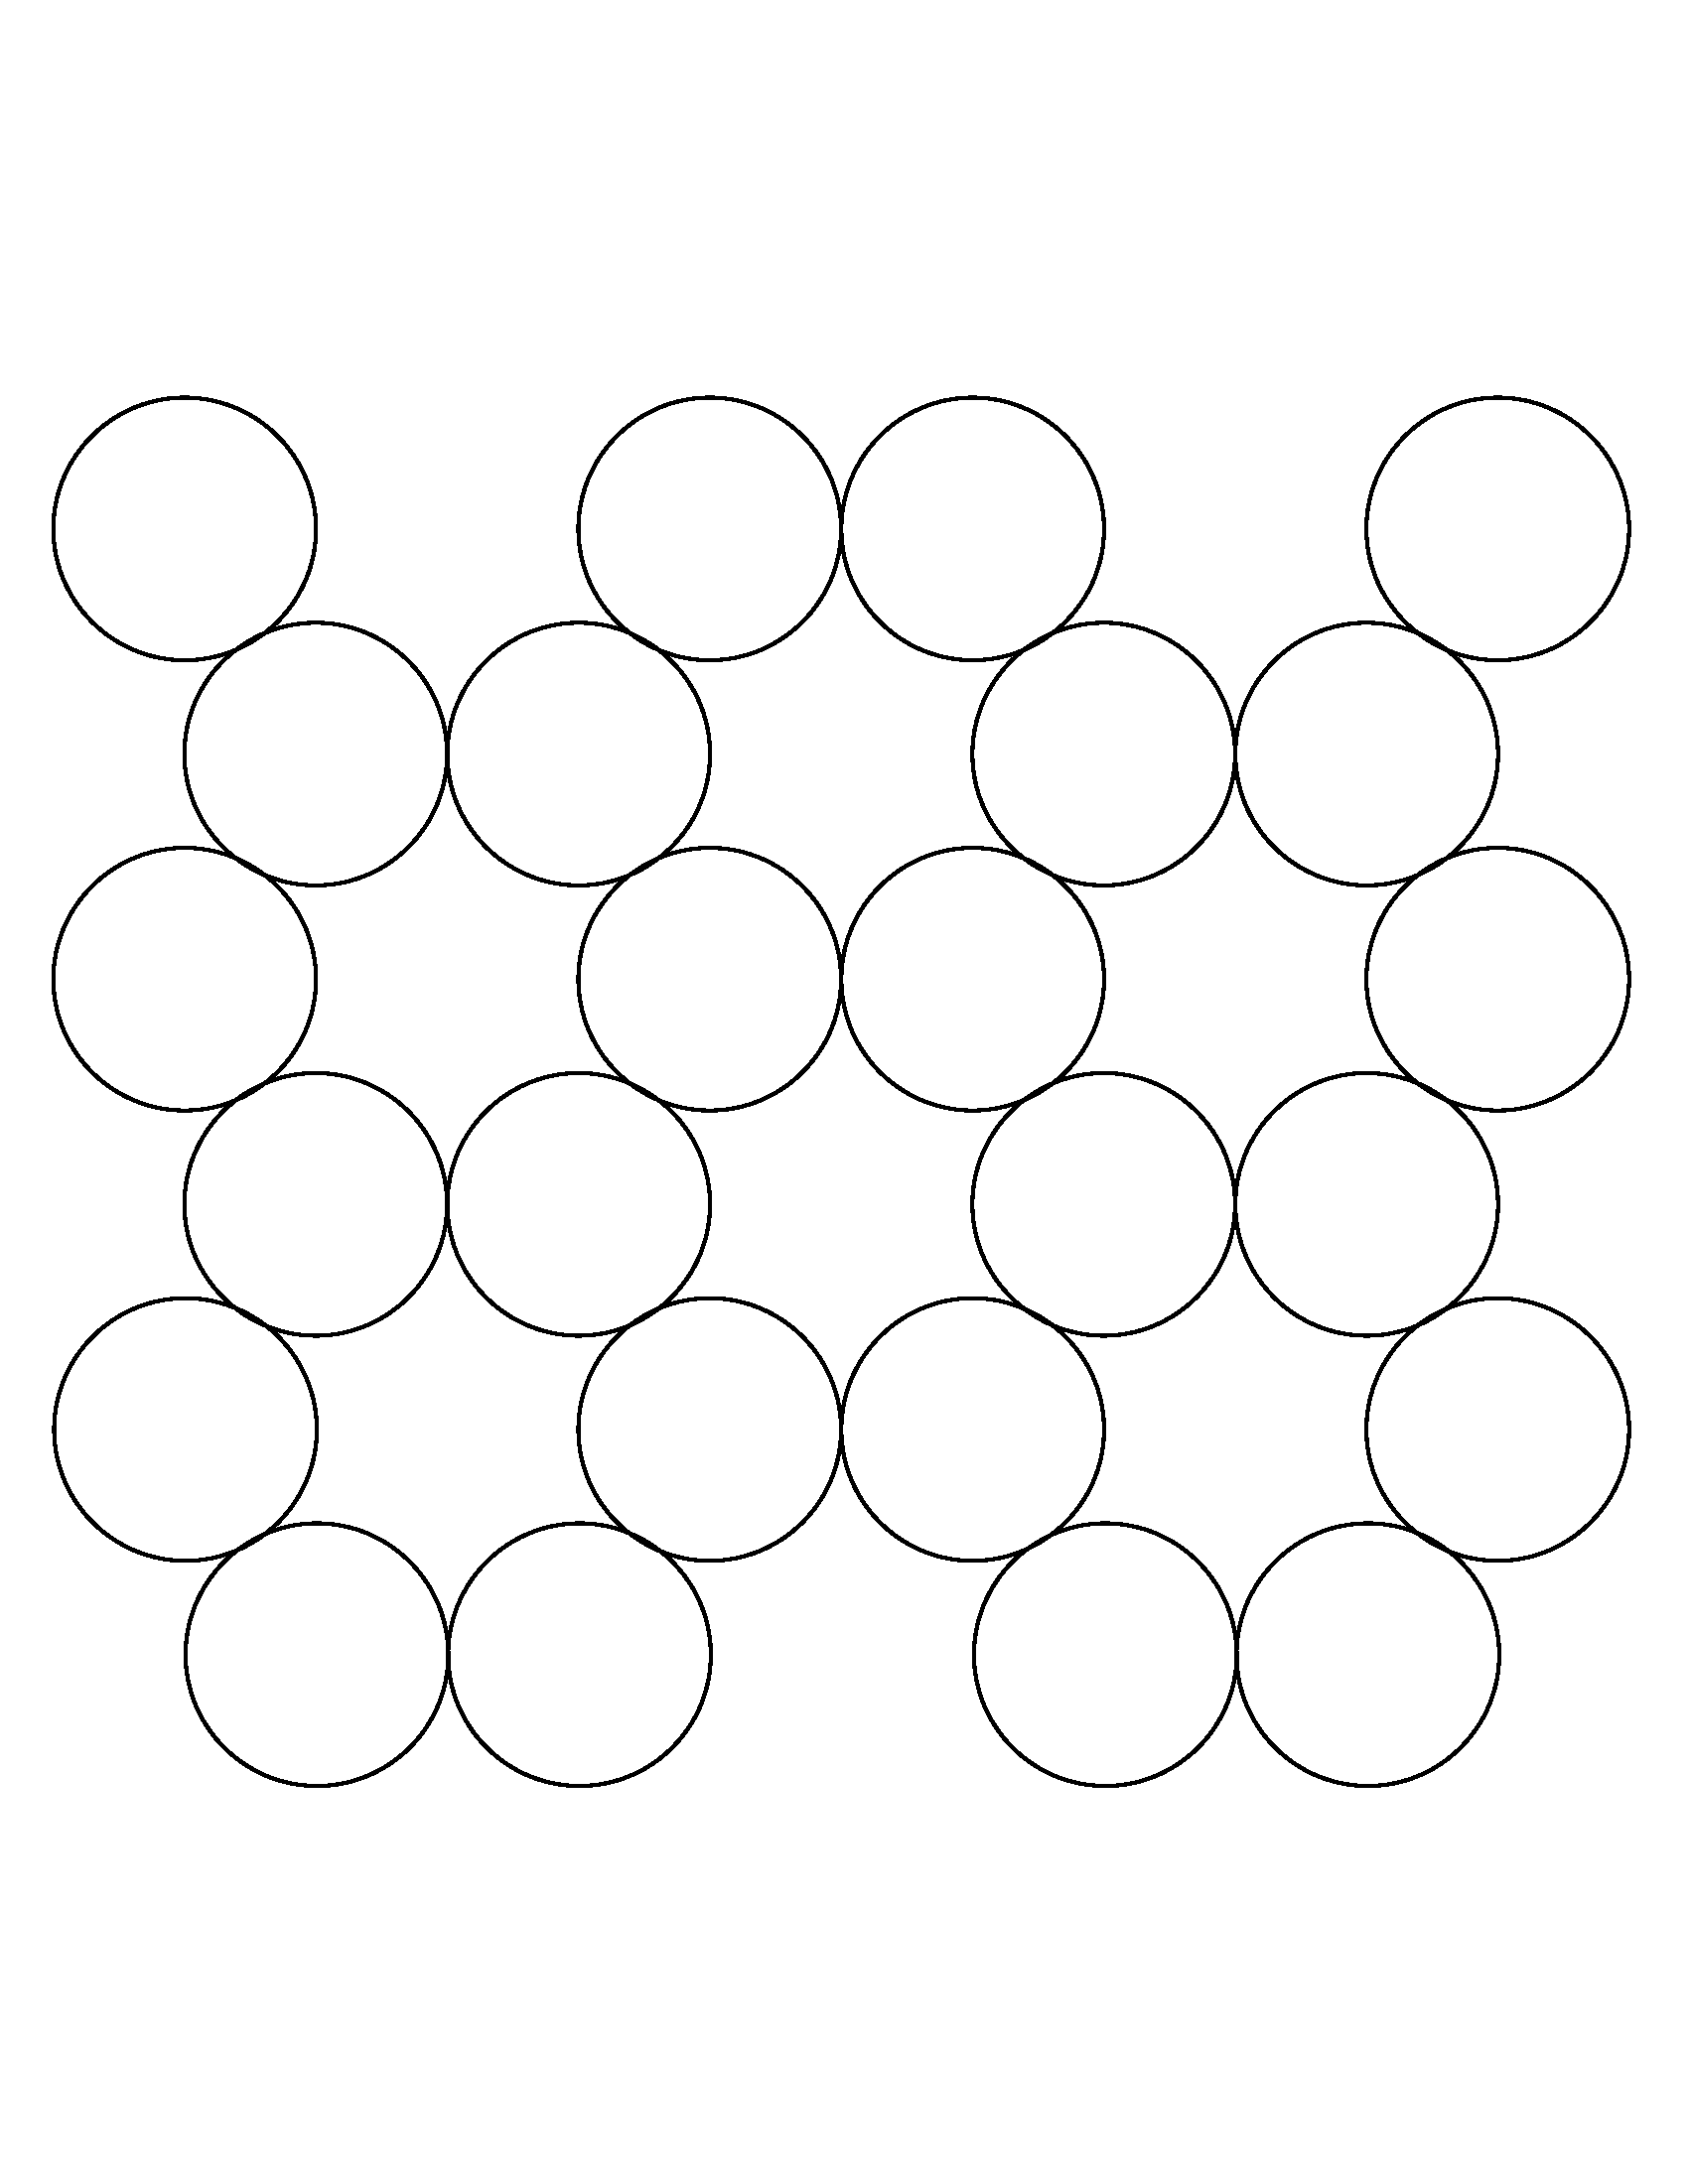
\includegraphics[width=2.7cm]{img/hex.png}
%%        \label{fig:ARCHalphas_10}
%%    }
%%    \subfigure[ EfficientNet ]{
%%        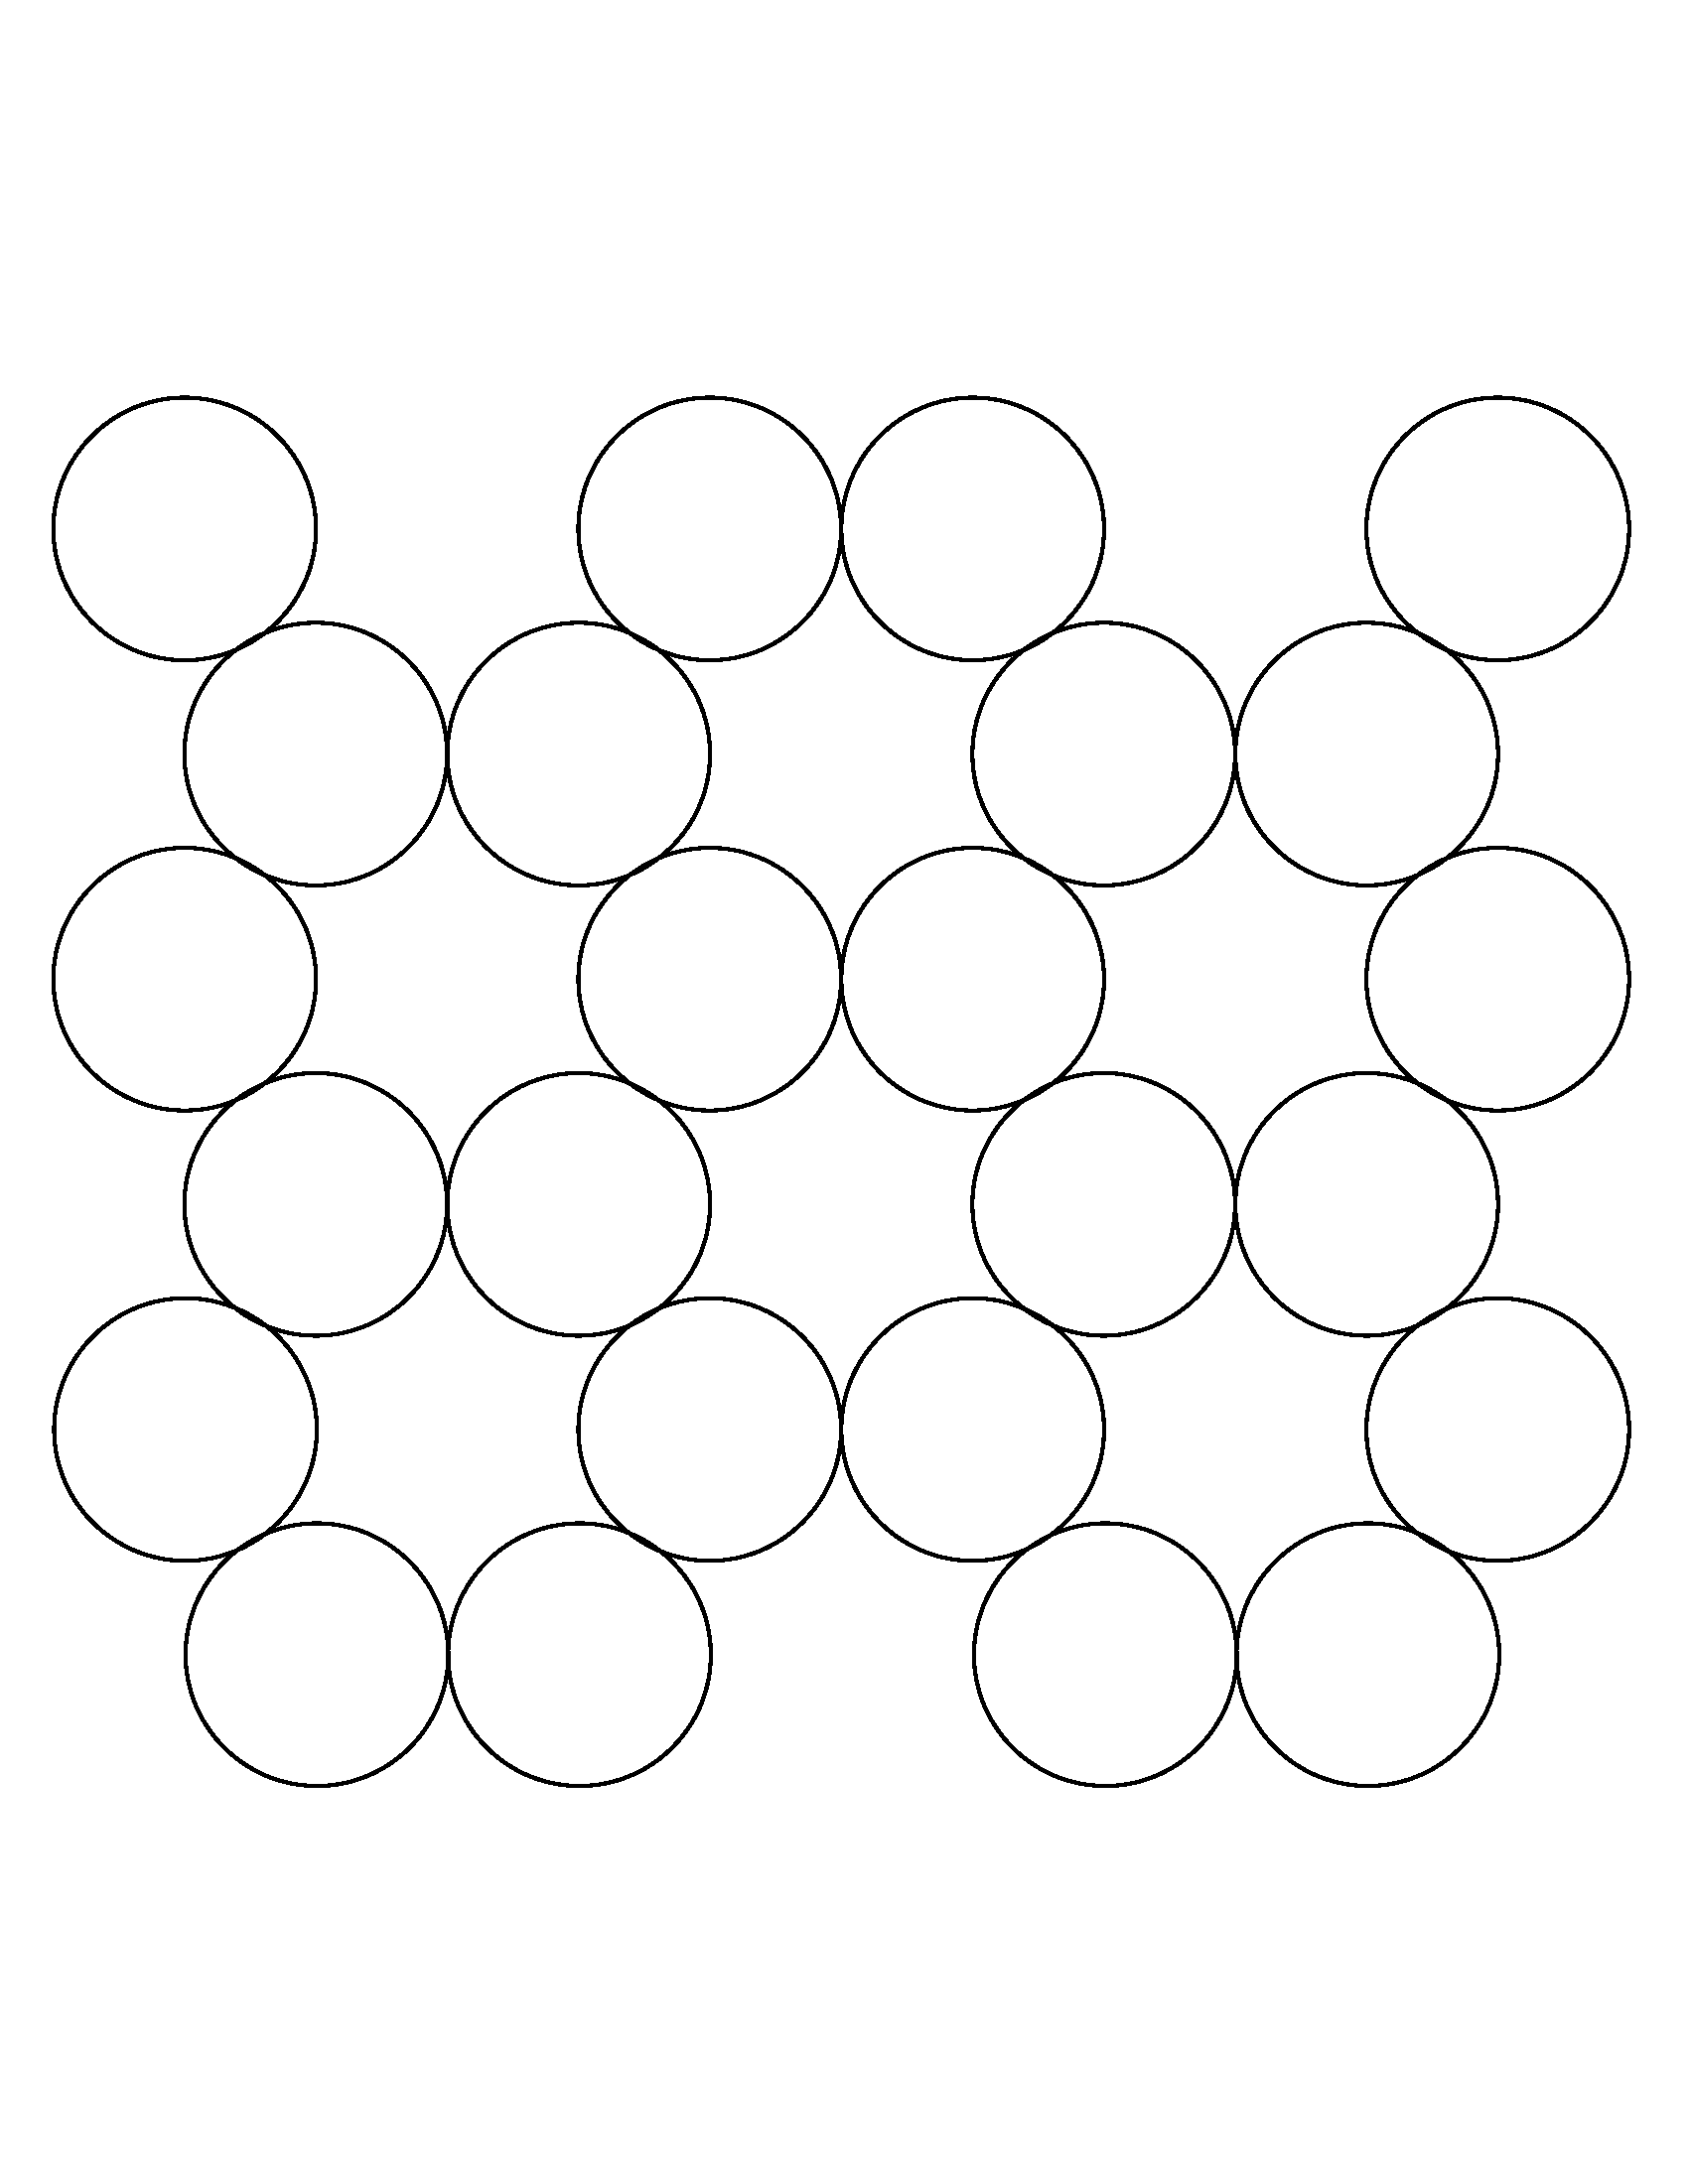
\includegraphics[width=2.7cm]{img/hex.png}
%%        \label{fig:ARCHalphas_11}
%%    }
%%    \subfigure[ SqueezeNext/SqNxt ]{
%%        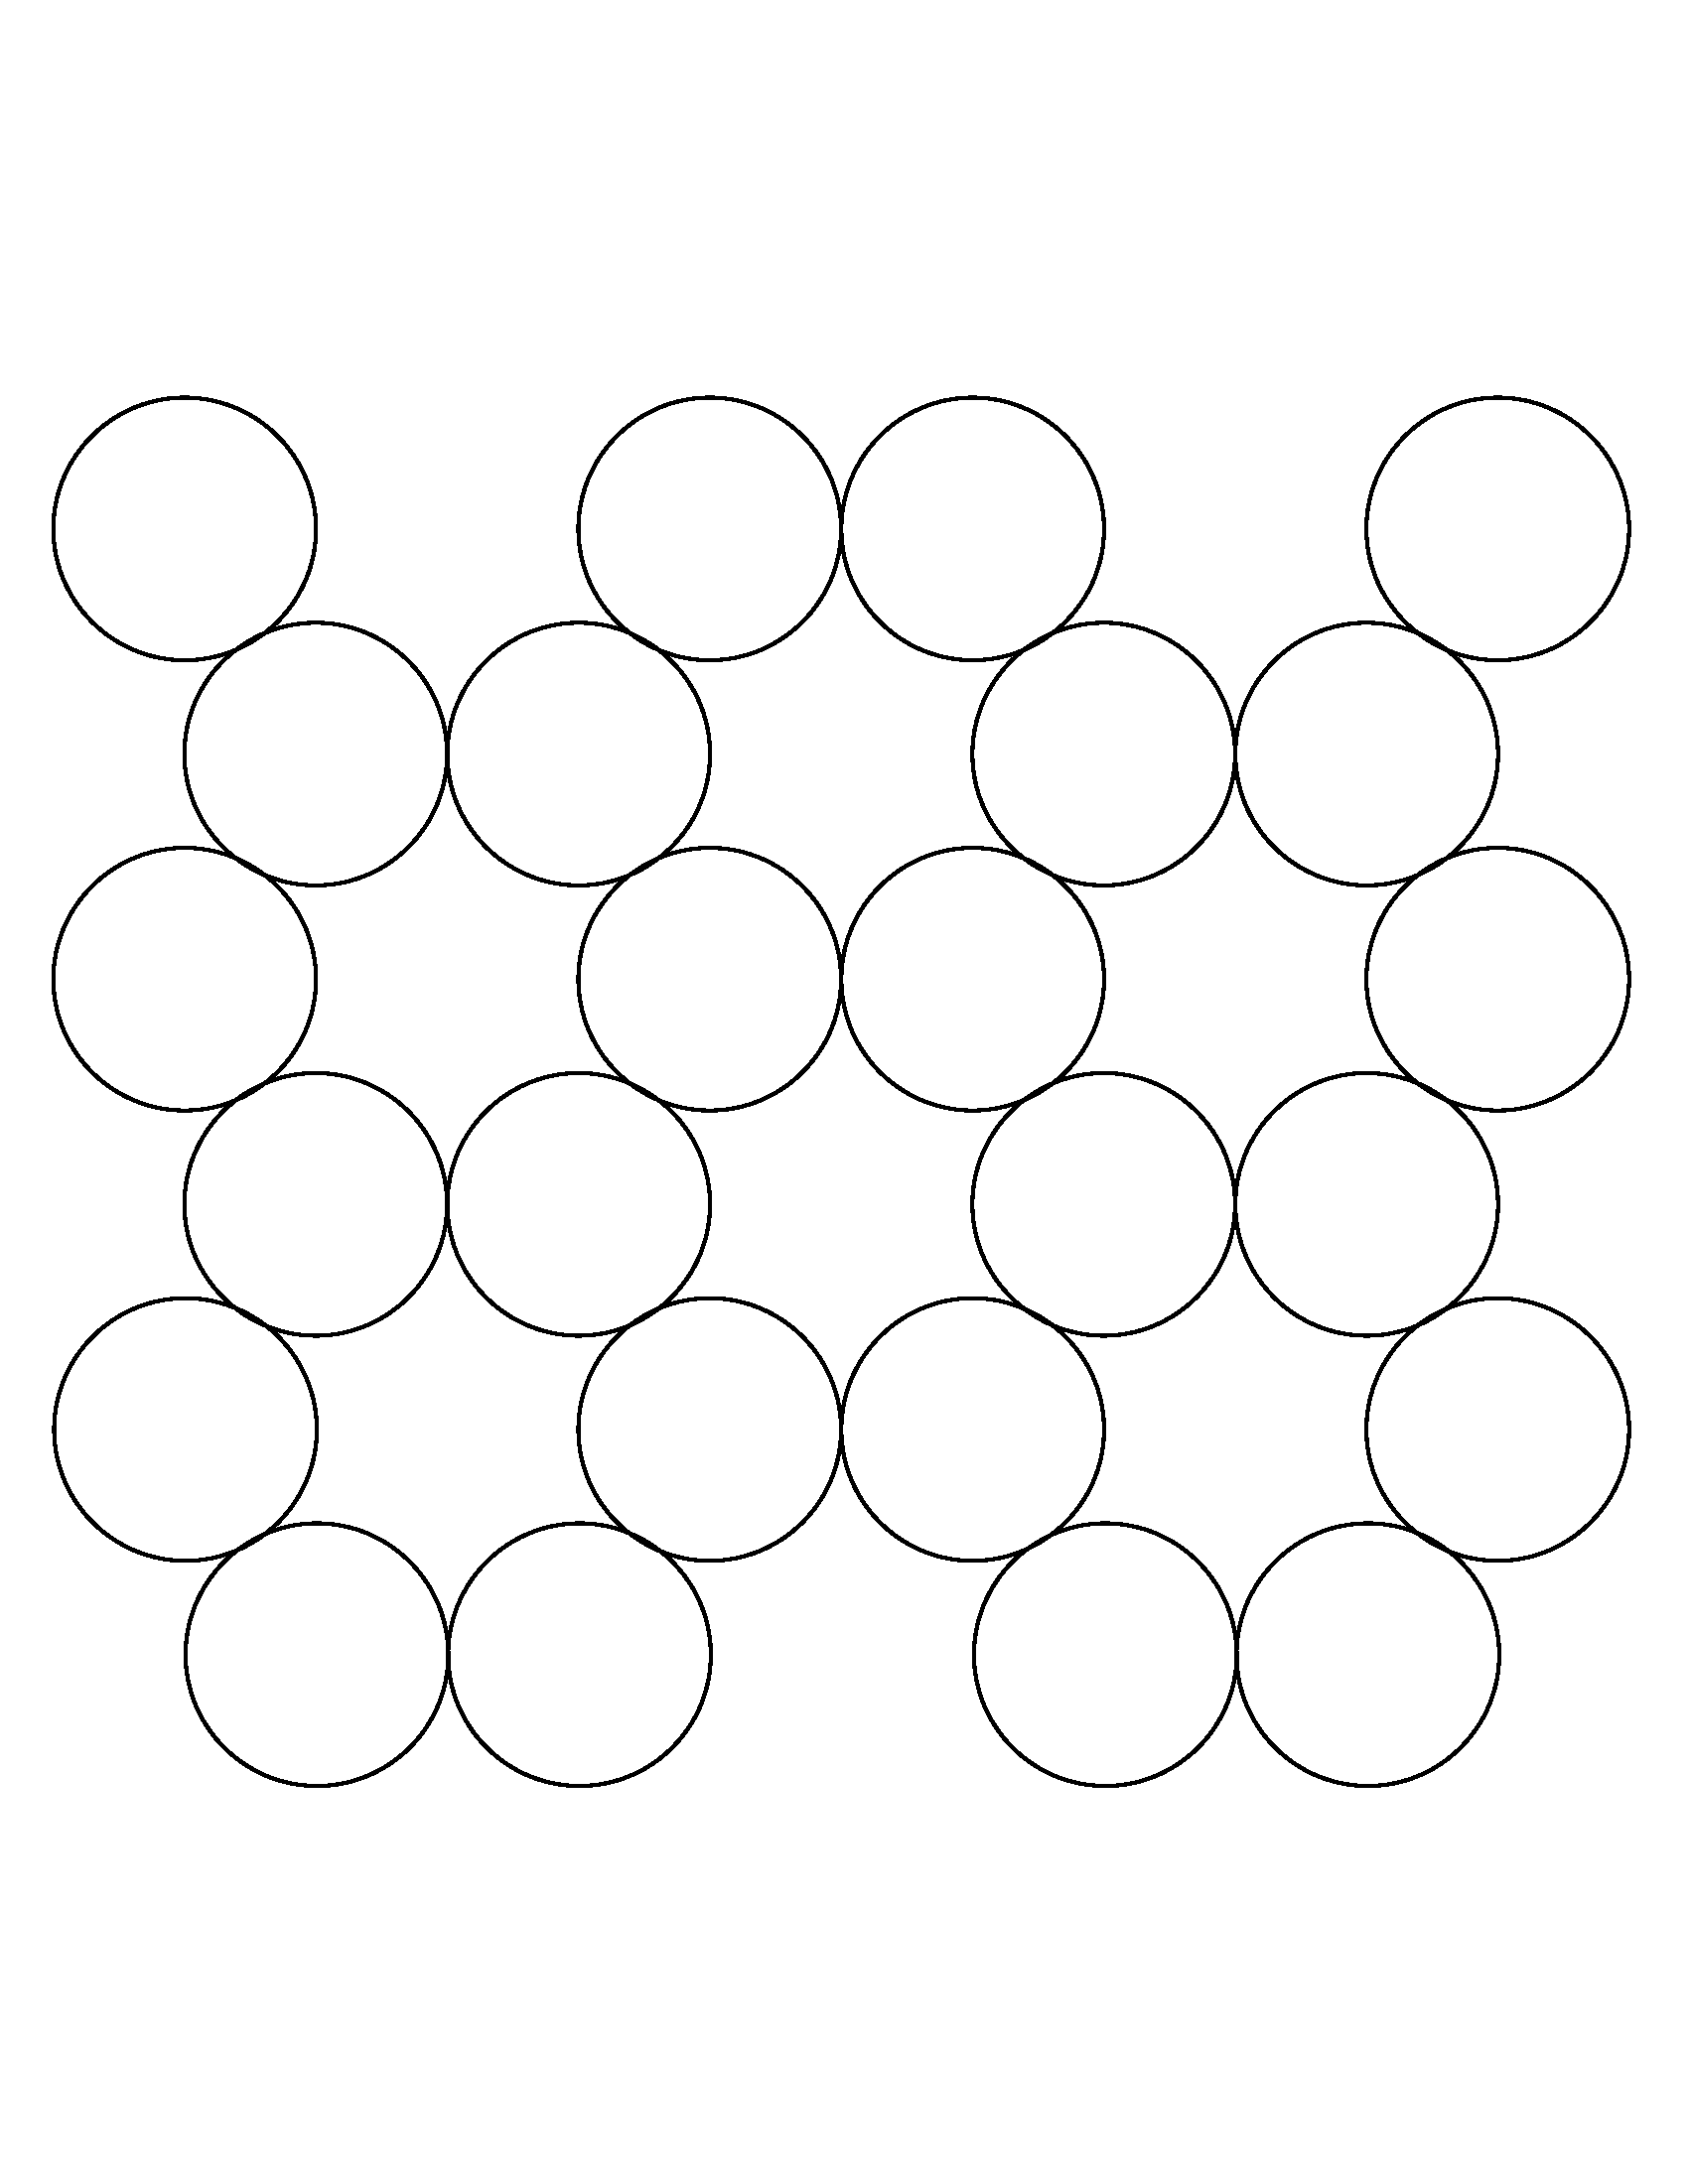
\includegraphics[width=2.7cm]{img/hex.png}
%%        \label{fig:ARCHalphas_12}
%%    }
%%    \subfigure[ ShuffleNet ]{
%%        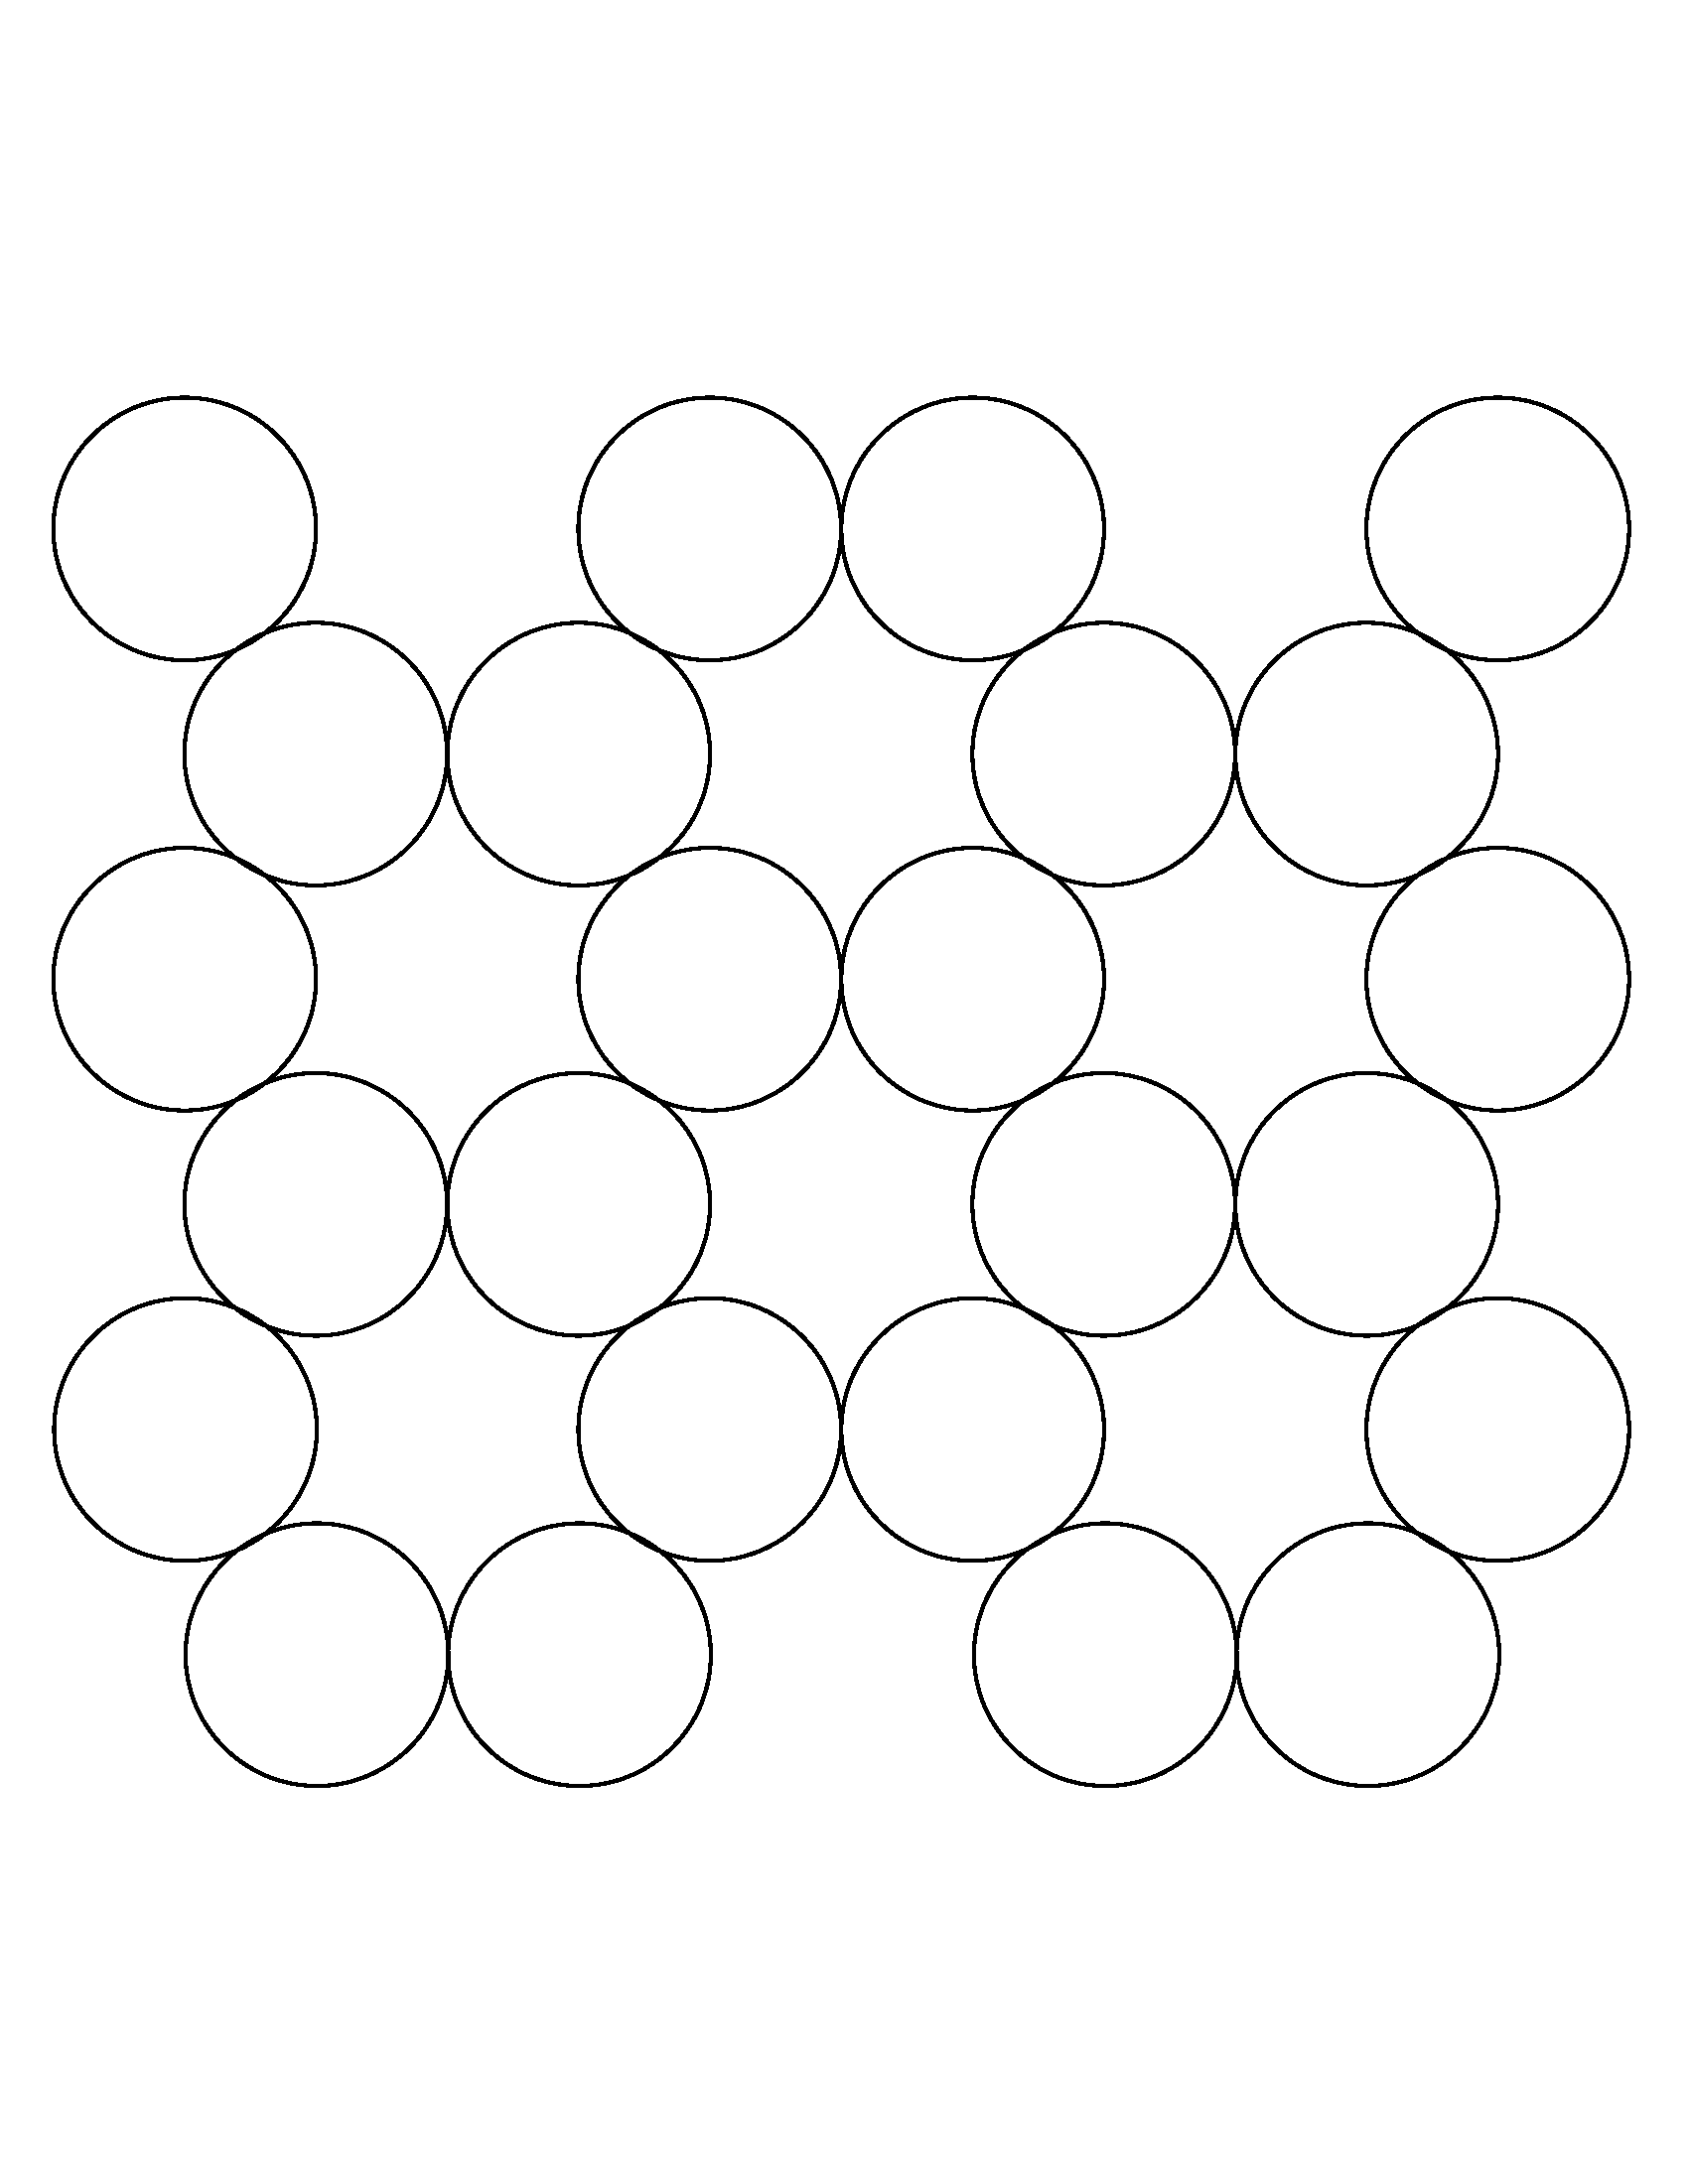
\includegraphics[width=2.7cm]{img/hex.png}
%%        \label{fig:ARCHalphas_13}
%%    }
%%    \subfigure[ DRN-C/DRN-D ]{
%%        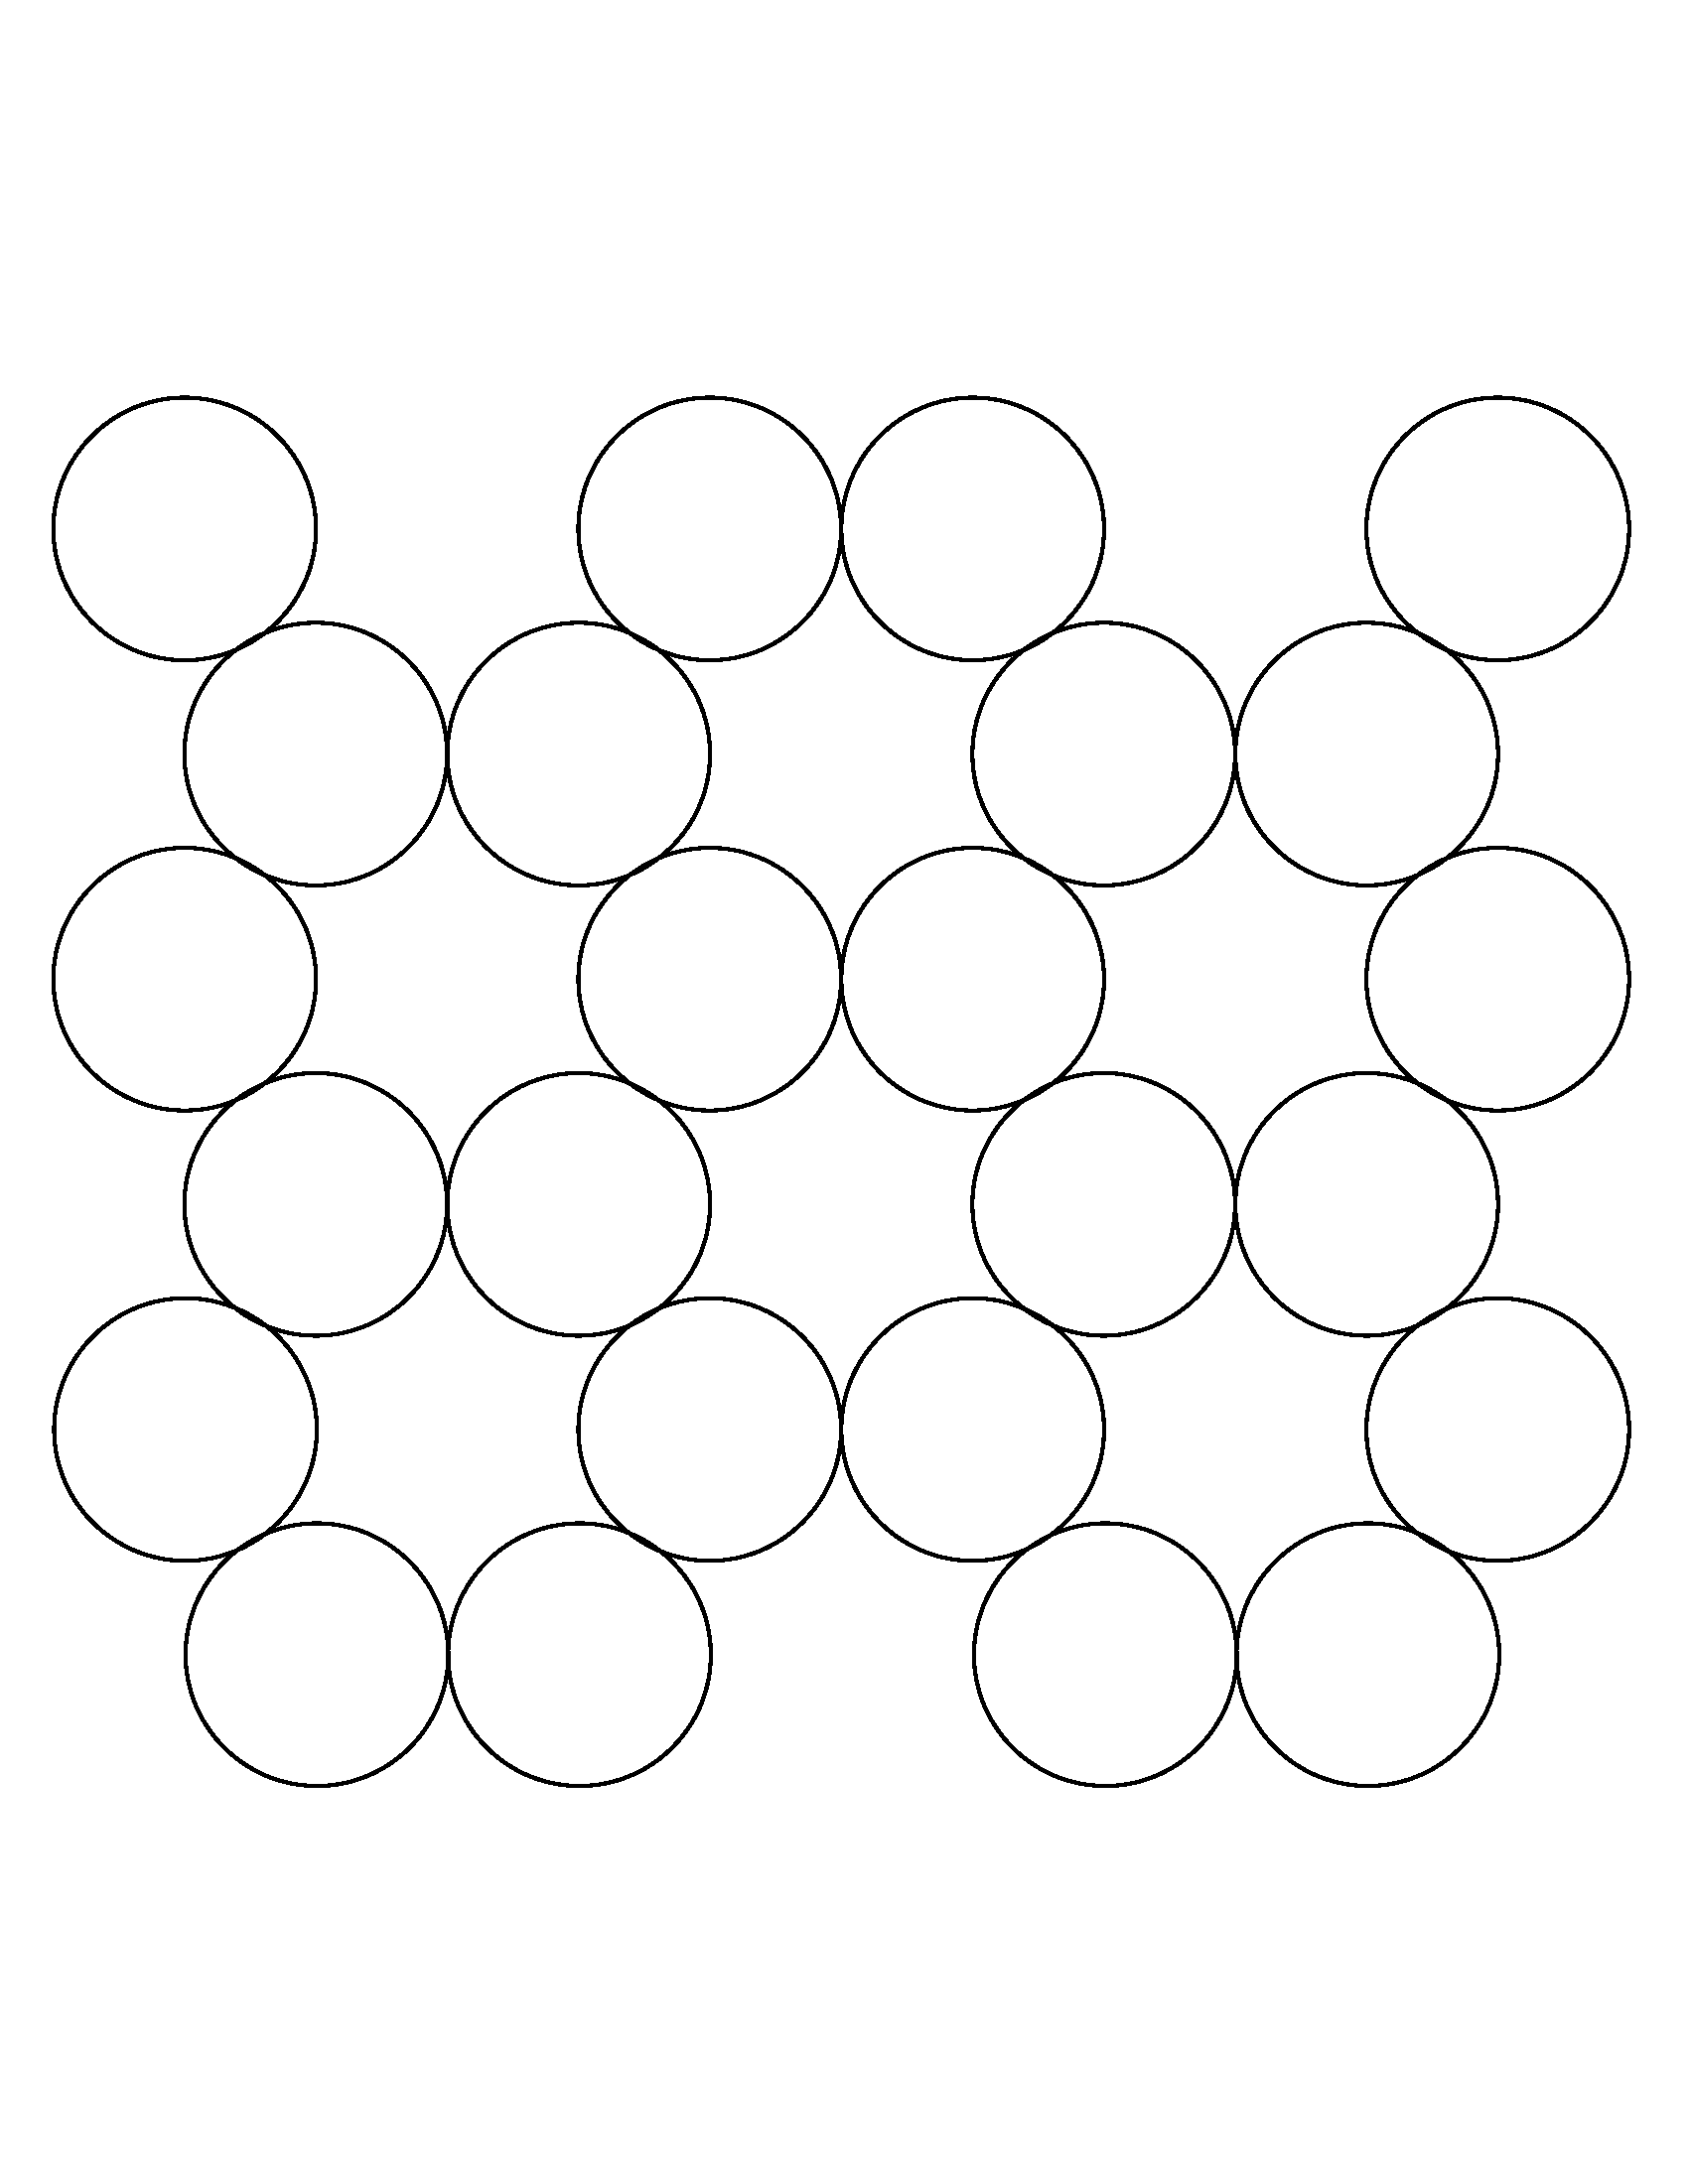
\includegraphics[width=2.7cm]{img/hex.png}
%%        \label{fig:ARCHalphas_14}
%%    }
%%    \subfigure[ ESPNetv2 ]{
%%        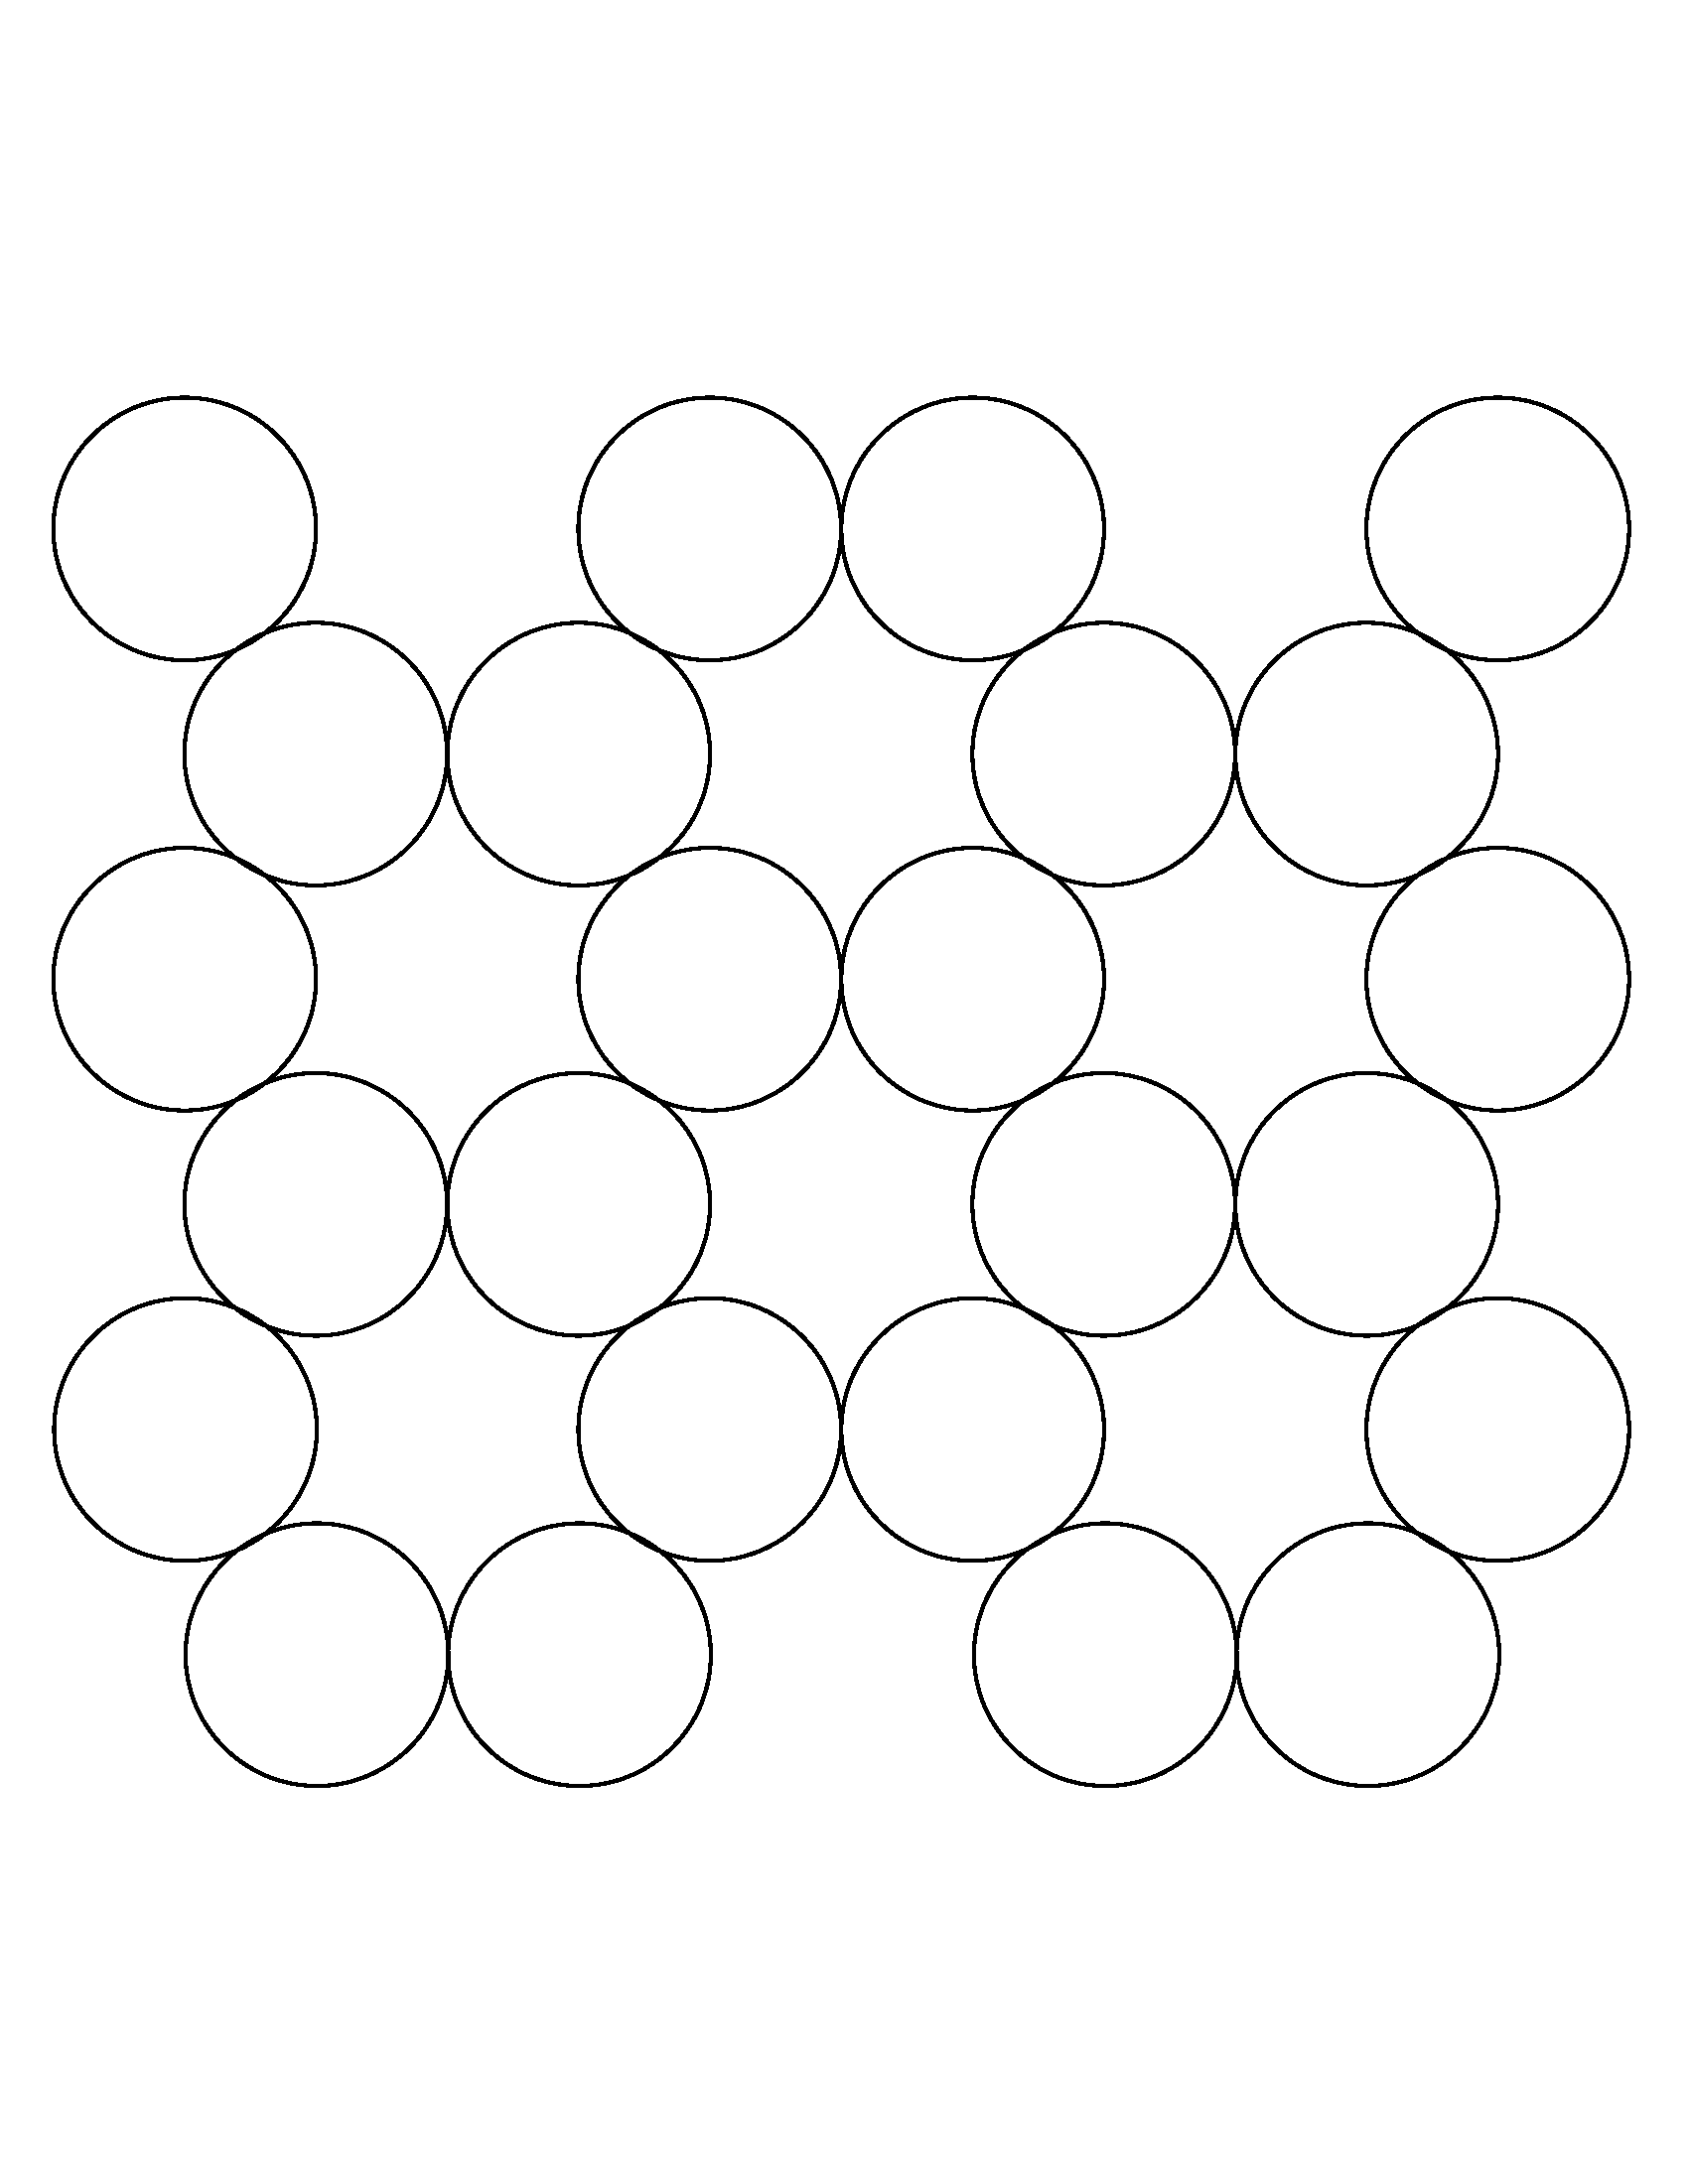
\includegraphics[width=2.7cm]{img/hex.png}
%%        \label{fig:ARCHalphas_15}
%%    }
%%    \subfigure[ HRNet ]{
%%        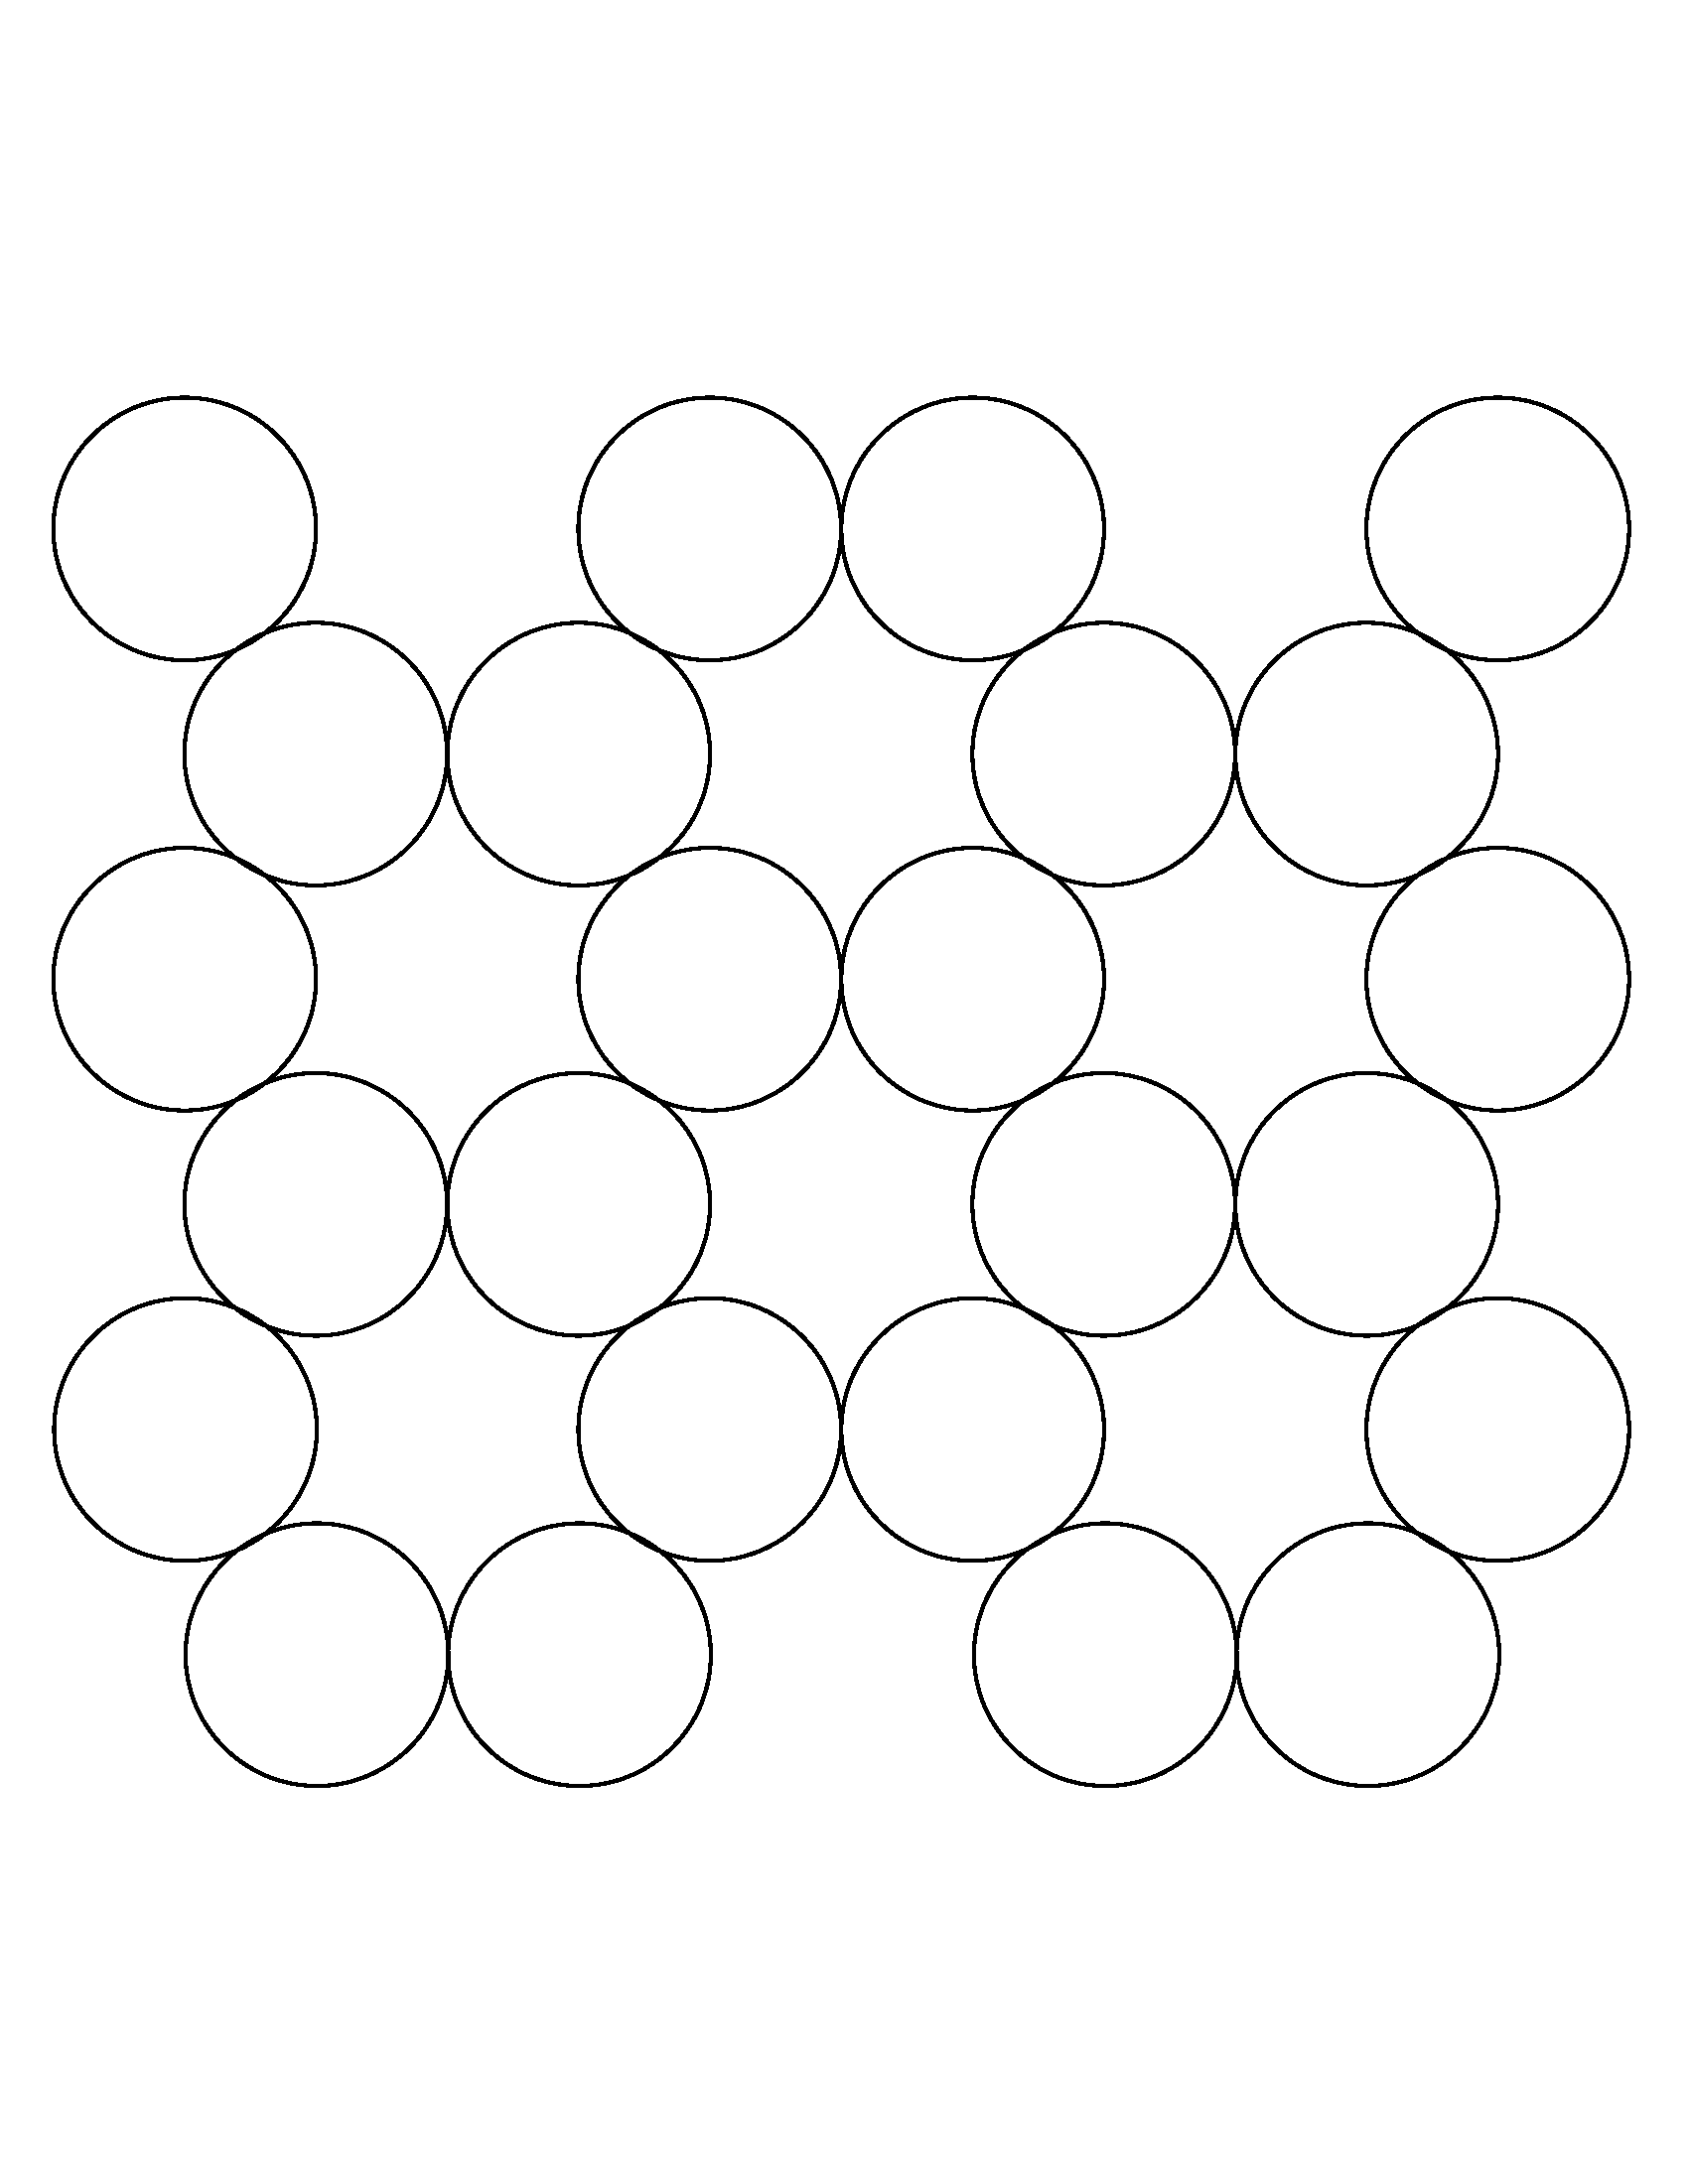
\includegraphics[width=2.7cm]{img/hex.png}
%%        \label{fig:ARCHalphas_16}
%%    }
%%    \subfigure[ SqueezeNet/SqueezeResNet ]{
%%        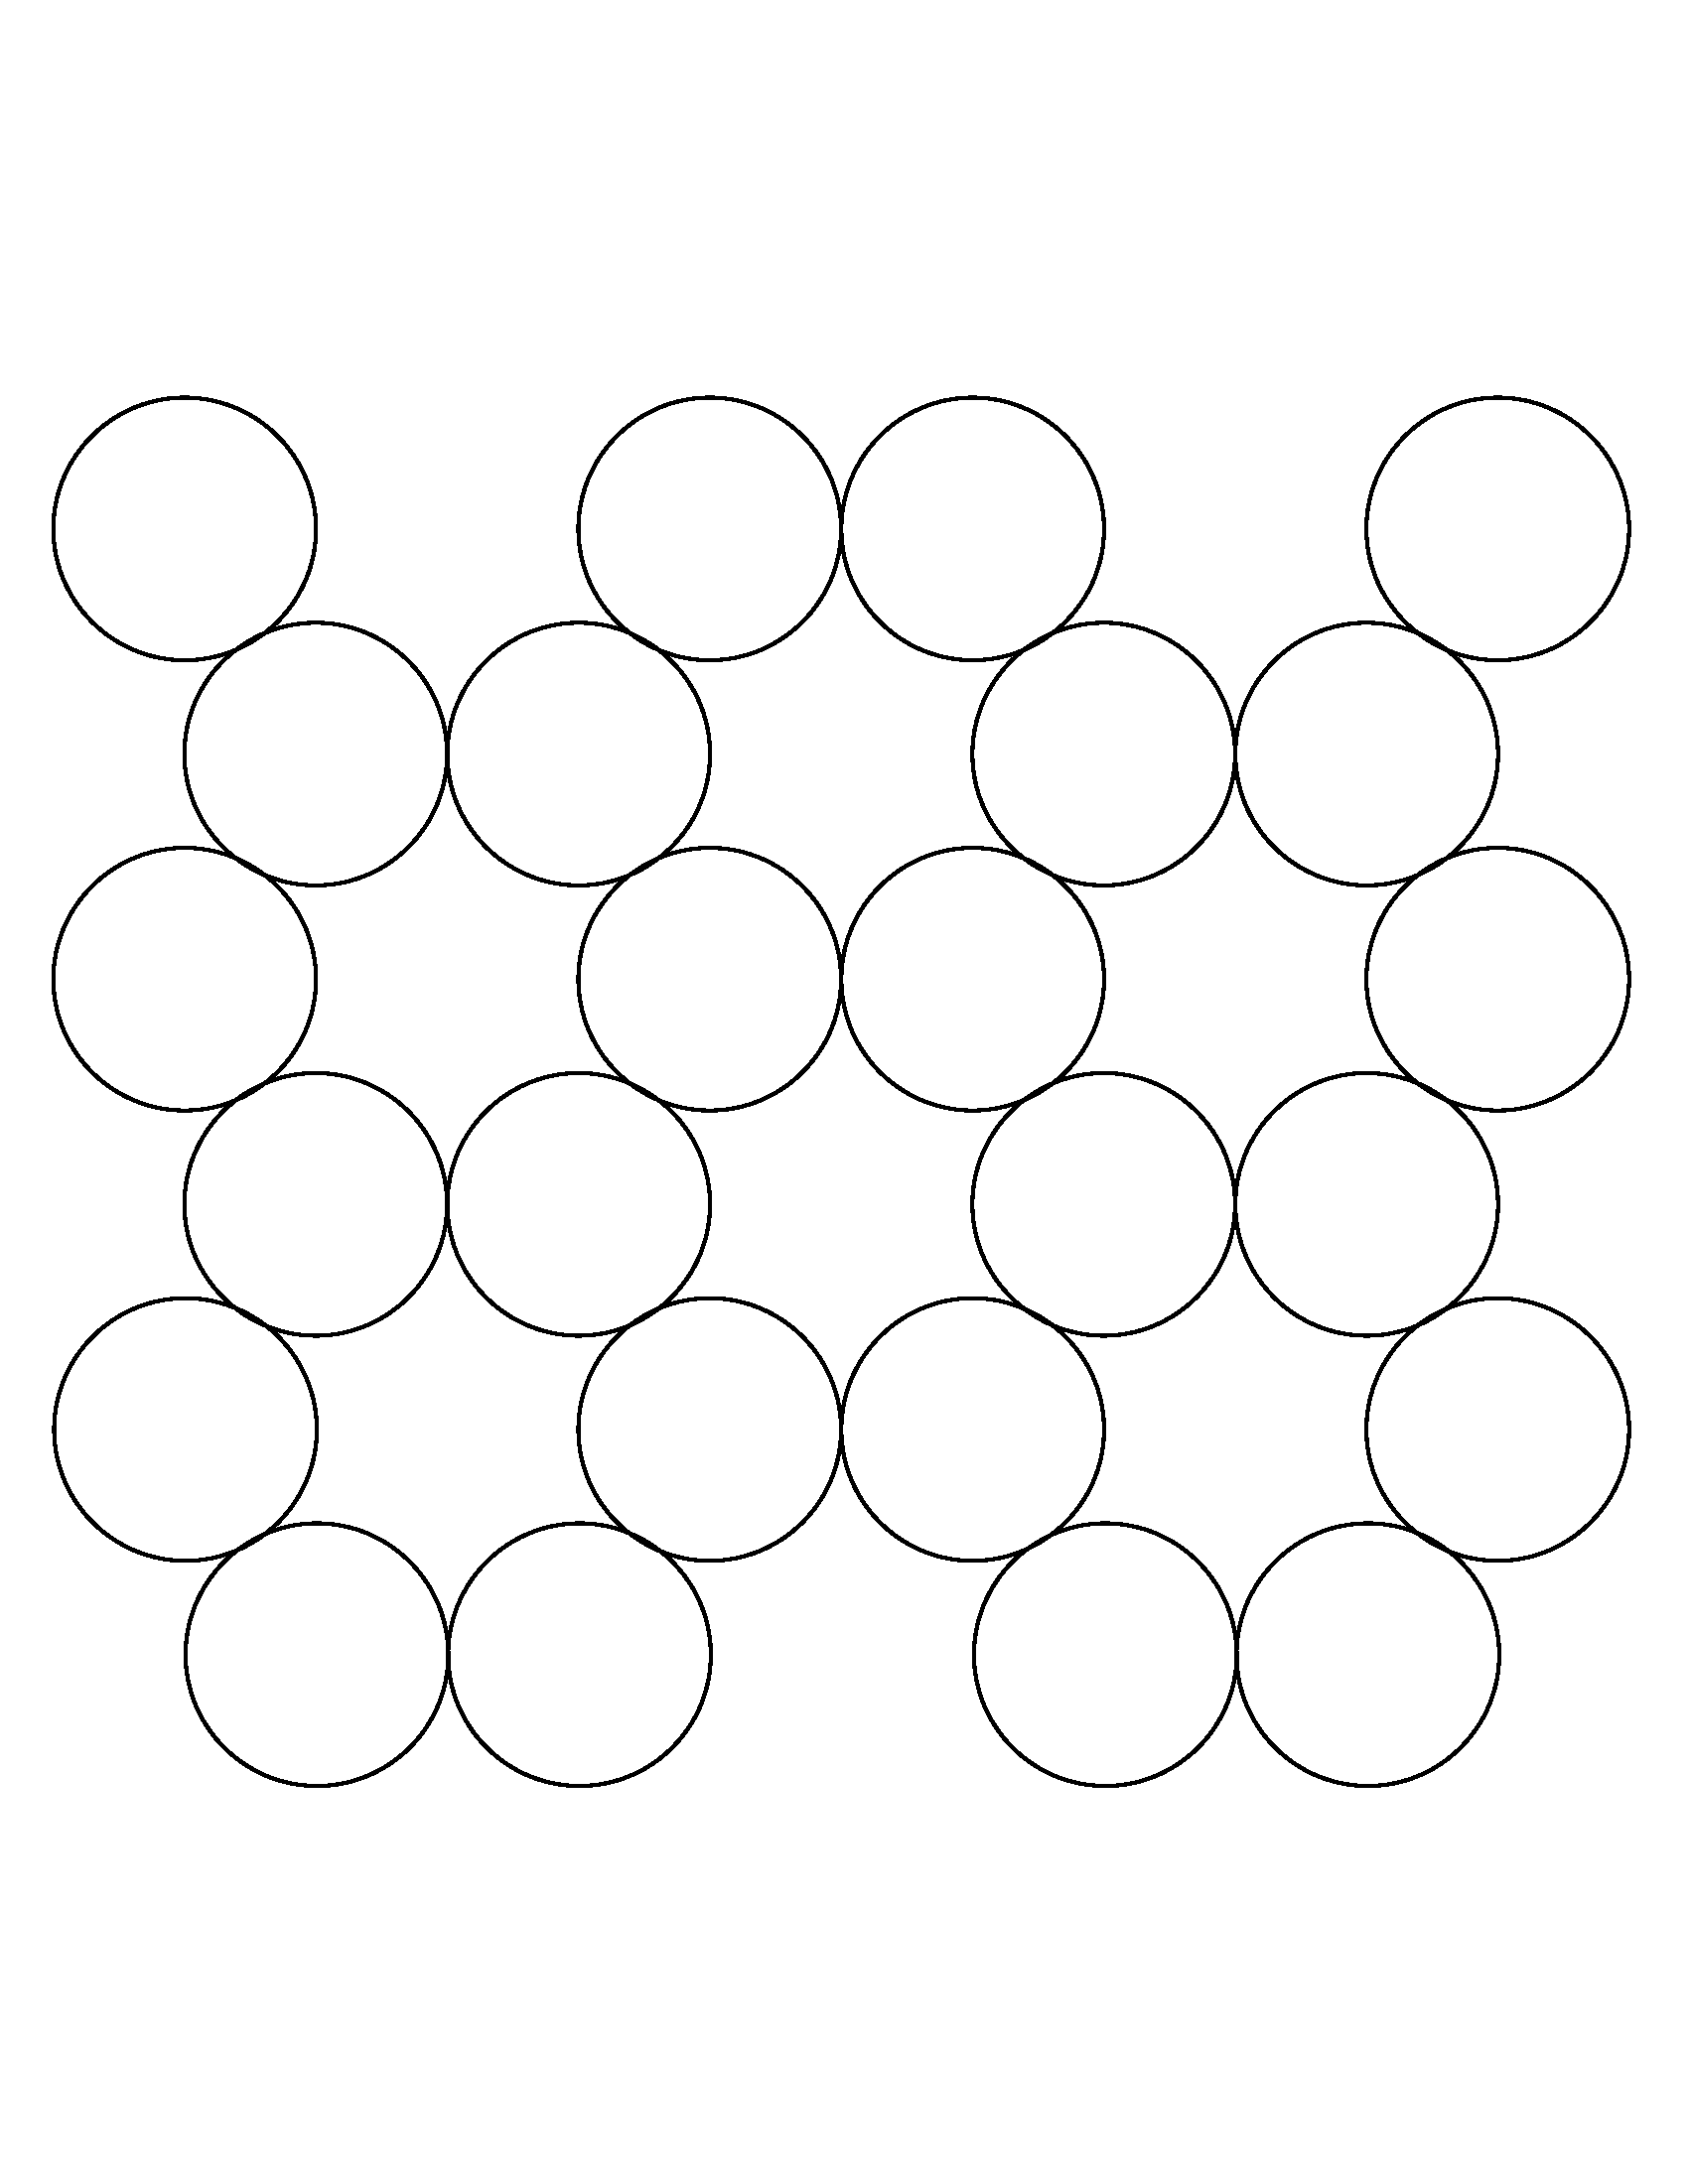
\includegraphics[width=2.7cm]{img/hex.png}
%%        \label{fig:ARCHalphas_17}
%%    }
%%    \caption{PL exponent $\alpha$ versus reported Top1 Test Accuracies for pretrained DNNs available for different architecture series (as segmented in Table~\ref{table:architectures}).
%%            }
%%    \label{fig:ARCHalphas}
%%\end{figure}



\begin{table}[t]
\small
\begin{center}
\begin{tabular}{|l|c|c|c|c|c|c|}
\hline
% MM: PRE CHANGE % Architecture & $\#$ of Models & Datasets & & & & \\
Architecture & $\#$ of Models & 
\multicolumn{5}{|c|}{ Datasets } \\
\hline

  & total &imagenet-1k & cifar-10 & cifar-100 & svhn & cub-200-2011 \\
\hline
ResNet & 51 &22 & 8 & 8 & 7 & 6 \\
EfficientNet & 20 &20 & 0 & 0 & 0 & 0 \\
PreResNet & 14 &14 & 0 & 0 & 0 & 0 \\
ShuffleNet & 12 &12 & 0 & 0 & 0 & 0 \\
VGG/BN-VGG & 12 &12 & 0 & 0 & 0 & 0 \\
DLA & 10 &10 & 0 & 0 & 0 & 0 \\
HRNet & 9 &9 & 0 & 0 & 0 & 0 \\
DRN-C/DRN-D & 7 &7 & 0 & 0 & 0 & 0 \\
SqueezeNext/SqNxt & 6 &6 & 0 & 0 & 0 & 0 \\
ESPNetv2 & 5 &5 & 0 & 0 & 0 & 0 \\
SqueezeNet/SqueezeResNet & 4 &4 & 0 & 0 & 0 & 0 \\
ProxylessNAS & 4 &4 & 0 & 0 & 0 & 0 \\
IGCV3 & 4 &4 & 0 & 0 & 0 & 0 \\
DIA-ResNet/DIA-PreResNet & 24 &0 & 8 & 8 & 8 & 0 \\
SENet/SE-ResNet & 20 &0 & 5 & 5 & 4 & 6 \\
WRN & 8 &0 & 0 & 4 & 4 & 0 \\
ResNeXt & 4 &0 & 0 & 0 & 4 & 0 \\

\hline
\end{tabular}
\end{center}
\caption{Architectures used in total and per dataset}
\label{table:architectures}
\end{table}




\begin{table}[t]
\scriptsize
\begin{center}
\begin{tabular}{|c|c|c|c|c|c|}
\hline
Dataset & Model  & $\langle\log\Vert\cdot\Vert^{2}_{F}\rangle$ & $\langle\log\Vert\cdot\Vert^{2}_{\infty}\rangle$ & $\hat{\alpha}$ & $\langle\log\Vert\cdot\Vert^{\alpha}_{\alpha}\rangle$ \\

\hline
 imagenet-1k & ResNet  & 2.52 &  3.35 & \textbf{1.91} & 2.04 \\
 imagenet-1k & EfficientNet  & 1.64 &  \textbf{1.11} & 1.60 & 1.58 \\
 imagenet-1k & PreResNet  & 2.57 &  3.93 & \textbf{1.90} & 1.93 \\
 imagenet-1k & VGG  & 0.92 &  \textbf{0.83} & 1.37 & 1.26 \\
 imagenet-1k & ShuffleNet  & 5.95 &  9.46 & 4.42 & \textbf{4.30} \\
 imagenet-1k & DLA  & 4.79 &  \textbf{3.02} & 3.94 & 4.06 \\
 imagenet-1k & HRNet  & 0.68 &  0.72 & \textbf{0.40} & 0.40 \\
 imagenet-1k & DRN-C  & 0.77 &  0.81 & \textbf{0.64} & 0.69 \\
 imagenet-1k & SqueezeNext  & 4.68 &  4.62 & 3.65 & \textbf{3.64} \\
 imagenet-1k & ESPNetv2  & 3.71 &  3.84 & \textbf{1.37} & 1.59 \\
 imagenet-1k & SqueezeNet  & 0.33 &  0.33 & \textbf{0.26} & 0.29 \\
 imagenet-1k & IGCV3  & 1.39 &  9.37 & 2.91 & \textbf{1.04} \\
 imagenet-1k & ProxylessNAS  & \textbf{0.44} &  0.51 & 0.53 & 0.51 \\
\hline
 cifar-10 & ResNet  & 0.56 &  0.55 & \textbf{0.53} & 0.53 \\
 cifar-10 & DIA-ResNet  & \textbf{0.22} &  0.28 & 0.53 & 0.56 \\
 cifar-10 & SENet  & 0.30 &  0.30 & \textbf{0.20} & 0.20 \\
\hline
 cifar-100 & ResNet  & 2.03 &  2.12 & \textbf{1.75} & 1.75 \\
 cifar-100 & DIA-ResNet  & \textbf{0.60} &  1.17 & 0.96 & 1.01 \\
 cifar-100 & SENet  & 0.60 &  0.65 & \textbf{0.51} & 0.51 \\
 cifar-100 & WRN  & 0.37 &  0.44 & 0.26 & \textbf{0.25} \\
\hline
 svhn & ResNet  & 0.20 &  0.20 & \textbf{0.15} & 0.16 \\
 svhn & DIA-ResNet  & 0.07 &  \textbf{0.06} & 0.13 & 0.13 \\
 svhn & SENet  & \textbf{0.04} &  0.07 & 0.05 & 0.05 \\
 svhn & WRN  & 0.07 &  0.08 & 0.07 & \textbf{0.07} \\
 svhn & ResNeXt  & 0.06 &  \textbf{0.06} & 0.11 & 0.09 \\
\hline
 cub-200-2011 & ResNet  & 0.45 &  \textbf{0.42} & 1.79 & 1.79 \\
 cub-200-2011 & SENet  & \textbf{1.03} &  1.13 & 1.36 & 1.40 \\

\hline
\end{tabular}
\vspace{-5mm}
\end{center}
\caption{RMSE Results for our analysis of all CV models in Table~\ref{table:datasets}. }
\label{table:RMSEresults}
\end{table}



\begin{table}[t]
\scriptsize
\begin{center}
\begin{tabular}{|c|c|c|c|c|c|}
\hline
Dataset & Model  & $\langle\log\Vert\cdot\Vert^{2}_{F}\rangle$ & $\langle\log\Vert\cdot\Vert^{2}_{\infty}\rangle$ & $\hat{\alpha}$ & $\langle\log\Vert\cdot\Vert^{\alpha}_{\alpha}\rangle$ \\

\hline
imagenet-1k & EfficientNet  & 0.65 & \textbf{0.84} & 0.67 & 0.67 \\
imagenet-1k & ResNet  & 0.77 & 0.61 & \textbf{0.87} & 0.86 \\
imagenet-1k & PreResNet  & 0.73 & 0.36 & \textbf{0.85} & \textbf{0.85} \\
imagenet-1k & ShuffleNet  & 0.63 & 0.06 & 0.80 & \textbf{0.81} \\
imagenet-1k & VGG  & 0.63 & \textbf{0.75} & 0.27 & 0.35 \\
imagenet-1k & DLA  & 0.11 & \textbf{0.65} & 0.40 & 0.36 \\
imagenet-1k & HRNet  & 0.91 & 0.90 & \textbf{0.97} & \textbf{0.97} \\
imagenet-1k & DRN-C  & 0.81 & 0.79 & \textbf{0.87} & 0.85 \\
imagenet-1k & SqueezeNext  & 0.05 & 0.07 & 0.42 & \textbf{0.43} \\
imagenet-1k & ESPNetv2  & 0.42 & 0.38 & \textbf{0.92} & 0.89 \\
imagenet-1k & ProxylessNAS  & \textbf{0.68} & 0.56 & 0.53 & 0.58 \\
imagenet-1k & IGCV3  & 0.98 & 0.12 & 0.92 & \textbf{0.99} \\
imagenet-1k & SqueezeNet  & 0.01 & 0.00 & \textbf{0.38} & 0.26 \\
\hline
cifar-10 & ResNet  & 0.58 & 0.59 & \textbf{0.62} & 0.61 \\
cifar-10 & DIA-ResNet  & \textbf{0.96} & 0.93 & 0.74 & 0.71 \\
cifar-10 & SENet  & 0.91 & 0.91 & \textbf{0.96} & \textbf{0.96} \\
\hline
cifar-100 & ResNet  & 0.61 & 0.58 & \textbf{0.71} & \textbf{0.71} \\
cifar-100 & DIA-ResNet  & \textbf{0.96} & 0.85 & 0.90 & 0.89 \\
cifar-100 & SENet  & 0.97 & 0.96 & \textbf{0.98} & \textbf{0.98} \\
cifar-100 & WRN  & 0.32 & 0.04 & 0.66 & \textbf{0.69} \\
\hline
svhn & ResNet  & 0.69 & 0.70 & \textbf{0.82} & 0.81 \\
svhn & DIA-ResNet  & 0.94 & \textbf{0.95} & 0.78 & 0.77 \\
svhn & SENet  & \textbf{0.99} & 0.96 & 0.98 & 0.98 \\
svhn & WRN  & 0.13 & 0.10 & 0.20 & \textbf{0.21} \\
svhn & ResNeXt  & 0.87 & \textbf{0.90} & 0.64 & 0.75 \\
\hline
cub-200-2011 & ResNet  & 0.94 & \textbf{0.95} & 0.08 & 0.08 \\
cub-200-2011 & SENet  & \textbf{0.66} & 0.59 & 0.41 & 0.38 \\

\hline
\end{tabular}
\vspace{-5mm}
\end{center}
\caption{R2 Results for our analysis of all CV models in Table~\ref{table:datasets}. }
\label{table:R2results}
\end{table}



\begin{table}[t]
\scriptsize
\begin{center}
\begin{tabular}{|c|c|c|c|c|c|}
\hline
Dataset & Model  & $\langle\log\Vert\cdot\Vert^{2}_{F}\rangle$ & $\langle\log\Vert\cdot\Vert^{2}_{\infty}\rangle$ & $\hat{\alpha}$ & $\langle\log\Vert\cdot\Vert^{\alpha}_{\alpha}\rangle$ \\

\hline
imagenet-1k & EfficientNet  & 0.67 & \textbf{0.79} & 0.66 & 0.66 \\
imagenet-1k & ResNet  & 0.78 & 0.70 & \textbf{0.91} & 0.89 \\
imagenet-1k & PreResNet  & 0.65 & 0.54 & \textbf{0.87} & \textbf{0.87} \\
imagenet-1k & ShuffleNet  & 0.39 & 0.09 & \textbf{0.85} & 0.82 \\
imagenet-1k & VGG  & 0.73 & \textbf{0.79} & 0.42 & 0.52 \\
imagenet-1k & DLA  & 0.51 & \textbf{0.82} & 0.78 & 0.69 \\
imagenet-1k & HRNet  & 0.56 & 0.44 & \textbf{0.61} & \textbf{0.61} \\
imagenet-1k & DRN-C  & \textbf{0.90} & 0.81 & \textbf{0.90} & \textbf{0.90} \\
imagenet-1k & SqueezeNext  & 0.47 & -0.33 & \textbf{0.73} & \textbf{0.73} \\
imagenet-1k & ESPNetv2  & 0.00 & 0.80 & \textbf{1.00} & \textbf{1.00} \\
imagenet-1k & SqueezeNet  & 0.33 & 0.00 & \textbf{0.67} & \textbf{0.67} \\
imagenet-1k & IGCV3  & \textbf{1.00} & 0.00 & \textbf{1.00} & \textbf{1.00} \\
imagenet-1k & ProxylessNAS  & \textbf{0.33} & \textbf{0.33} & \textbf{0.33} & \textbf{0.33} \\
\hline
cifar-10 & ResNet  & 0.64 & 0.64 & \textbf{0.71} & \textbf{0.71} \\
cifar-10 & DIA-ResNet  & 0.79 & 0.50 & \textbf{0.86} & 0.79 \\
cifar-10 & SENet  & 0.74 & \textbf{0.95} & \textbf{0.95} & \textbf{0.95} \\
\hline
cifar-100 & ResNet  & \textbf{0.64} & 0.57 & \textbf{0.64} & \textbf{0.64} \\
cifar-100 & DIA-ResNet  & \textbf{0.93} & 0.43 & \textbf{0.93} & \textbf{0.93} \\
cifar-100 & SENet  & \textbf{1.00} & \textbf{1.00} & \textbf{1.00} & \textbf{1.00} \\
cifar-100 & WRN  & \textbf{0.67} & -0.67 & 0.00 & 0.00 \\
\hline
svhn & ResNet  & \textbf{0.81} & 0.71 & \textbf{0.81} & \textbf{0.81} \\
svhn & DIA-ResNet  & \textbf{0.86} & \textbf{0.86} & 0.57 & 0.57 \\
svhn & SENet  & \textbf{1.00} & \textbf{1.00} & 0.67 & 0.67 \\
svhn & WRN  & -0.33 & -0.33 & \textbf{0.67} & \textbf{0.67} \\
svhn & ResNeXt  & \textbf{0.67} & \textbf{0.67} & 0.33 & 0.33 \\
\hline
cub-200-2011 & ResNet  & \textbf{1.00} & \textbf{1.00} & -0.33 & -0.33 \\
cub-200-2011 & SENet  & \textbf{0.87} & \textbf{0.87} & -0.20 & -0.20 \\

\hline
\end{tabular}
\vspace{-5mm}
\end{center}
\caption{Kendal-$\tau$ Results for our analysis of all CV models in Table~\ref{table:datasets}. }
\label{table:Ktauresults}
\end{table}




%%\subsection{Supplementary Figures}
\subsection{Supplementary Tables and Figures}

\michael{Charles, would you put in a couple of paragraphs about how you generated the tables/figures in the appendix, and a few things we learn from them, i.e., basically enough to convince that reviewer that we paid attention to their concerns.}
\charles{fixed below}
\michael{Table~\ref{table:architectures} still needs to be fixed, since it does not include the overall results partitioned by dataset that we had in the old Table~\ref{table:datasets}. }

%To explain further how to reproduce our analysis, we run three batches of linear regressions. 
%First, at the global level, we divide models by datasets and run regressions separately on all models of a certain dataset, regardless of the architecture. 
%At this level, the plots are quite noisy and clustered, as each architecture has its own accuracy trend; but one can
% still see that most plots show positive relationship with positive coefficients. 
% V1 REMOVED FOR V2 % Example regressions are shown in Figure~\ref{fig:DSalphas}, as available in the results notebook.
%%Example regressions are shown in 
%%Figure~\ref{fig:DSalphas}, for models segmented by dataset, as listed in Table~\ref{table:datasets}, 
%%and in 
%%Figure~\ref{fig:ARCHalphas}, for models segmented by architecture, as listed in Table~\ref{table:architectures}.
%\michael{Charles, this paragraph is stale since it refers to the old figures that the reviewer did not like, so would you update it.}

Table~\ref{table:results} and Figures~\ref{fig:summary_regressions_A}-\ref{fig:summary_regressions_I} below present results for OLS 
(Ordinary Least Squares) regressions for every dataset and architecture series listed in Table~\ref{table:architectures},
 created by running the \texttt{WeightWatcher} tool (version 0.2.7)~\cite{weightwatcher_package}
on numerous pretrained models taken from the \texttt{OSMR/imgclsmob Sandbox} github repository of pretrained CV DNN model
ggithub repository. \michael{citation here ?}
In each Figure,  each row of subfigures, for a given pretrained model and dataset, depicts the average Norm-based and Power Law metrics
 ($\langle\log\Vert\cdot\Vert_{F}\rangle$,    $\langle\log\Vert\cdot\Vert_{\infty}\rangle$,
$\hat{\alpha}$,  $\langle\log\Vert\cdot\Vert^{\alpha}_{\alpha}\rangle$)
 against the Top1 Test Accuracy, as reported in the github repository README file~\cite{osmr} ),
along with a shaded area representing the $95\%$ confidence bound.
For each regression, we report the RMSE, R2 regresssion metrics, and Kendal-$\tau$ rank correlation metric,
both in the title of each subfiguire, and in Table~\ref{table:RMSEresults}, Table~\ref{table:R2results}, and Table~\ref{table:Ktauresults}, respectively.
To reproduce these Figures and Tables, see the \texttt{OSMR-Analysis.ipynb} python Jupyter Notebook, as listed in Table~\ref{},
and provided github repo accompanying this paper.
The reader may regenerate these Figures and Tables,
and even more fine grained results, by rerunning
 the \texttt{OSMR-Analysis.ipynb} python Jupyter Notebook (see Table~\ref{table:notebooks}), which 
analyzes the precomputed data in the \texttt{df\_all.xlsx} file. 
This repository also contains the original \texttt{Google Colab} notebooks, run in January 2020, 
which downloads the pretrained models and  and runs the \texttt{WeightWatcher} tool on them.
%To generate the results in Table~\ref{table:results}, we run linear regressions for each architecture series in Table~\ref{table:architectures}, regressing each empirical Log Norm metric against the reported Top1 rrors (as listed on the \texttt{osmr/imgclsmob} github repository README file~\cite{osmr}, with the relevant data extracted and provided in our github repo as \texttt{pytorchcv.html}).
%We record the $RMSE$, $R^{2}$, and Kendall-$\tau$ for each metric, averaged over all regressions for all architectures and datasets;
%see Table~\ref{table:RMSEresults}, Table~\ref{table:R2results}, and Table~\ref{table:Ktauresults}, respectively.
%captions fixed in table Ktau.  
%In the repo, plots are provided for every regression, and more fine grained results may be computed by the reader by analyzing the data in the \texttt{df\_all.xlsx} file.
The reader may also run the  \texttt{WeightWatcher} locally on each of the 
pretrained models,
such as the ResNet models, trained on the ImageNet-1K dataset, using the \texttt{WeightWatcher-ResNet-1K.ipynb} notebook.
(However, note that the models may have changed, giving slightly different results).
The final analysis includes 108 regressions in all.%, those with 4 or more models.%, with a positive $R^2$.
See Figure~\ref{fig:summary_regressions_A}-\ref{fig:summary_regressions_I} for more details.
%5Figure~\ref{fig:summary_regressions_B},
%Figure~\ref{fig:summary_regressions_C},
%Figure~\ref{fig:summary_regressions_D},
%Figure~\ref{fig:summary_regressions_E},
%Figure~\ref{fig:summary_regressions_F},
%Figure~\ref{fig:summary_regressions_G},
%Figure~\ref{fig:summary_regressions_H}, and

\michael{Charles, would you put a bit of discussion, e.g., on best and worst, again just a teaser to satisfy that reviewer.}
\charles{below}
From these Figures, we recognize fits of varying quality, ranging from remarkably good to completely uncorrelated.
Starting with the best, consider the Imagenet-1K PreResNet results.  Figure~\ref{fig:summary_regressions_A_10} shows 
the Avg. Log Spectral Norm $\langle\log\Vert\mathbf{W}\Vert^{2}_{\infty}\rangle$, 
which has a rather large $RMSE=3.93$, and rather small $R2=0.36$, and Kendal-$\tau=0.54$, and
has 6 out of 13 points outside the $95\%$ confidence bands.  In contrast, 
the Avg. Log Alpha Norm $\langle\log\Vert\mathbf{W}\Vert^{\alpha}_{\alpha}\rangle$, 
in  Figure~\ref{fig:summary_regressions_A_12} , 
has a much smaller $RMSE=1.93$, and much larger  $R2=0.85$, and Kendal-$\tau=0.87$, 
and only 2 points outside the $95\%$ confidence bands.
For examples of lower quality fits, consider the SqueezeNext results, as shown Figures~\ref{fig:summary_regressions_C_10} and 
~\ref{fig:summary_regressions_C_12}.  
The Avg. Log Spectral Norm $\langle\log\Vert\mathbf{W}\Vert^{2}_{\infty}\rangle$ appears
visually anti-correlated with the test accuracies
(as it is with ShuffleNet, in Figure ~\ref{fig:summary_regressions_B_02}).
It has a very large $95\%$ confidence band, with only 2 points close to the regression line, 
a large RMSE,  $R2=0.07$ (i.e zero), and small Kendal-$\tau=0.33$.  
The Avg. Log Alpha Norm $\langle\log\Vert\mathbf{W}\Vert^{\alpha}_{\alpha}\rangle$ is (as always) positively-correlated
with test accuracies, but with $R2=0.43$, show some linear correaltion, and a reasonable Kendal-$\tau=0.73$,
showing moderately strong rank correlation.


\begin{figure}[t]
    \centering
    \subfigure[ imagenet-1k--ResNet, $\langle\log\Vert\cdot\Vert_{F}\rangle$ ]{
        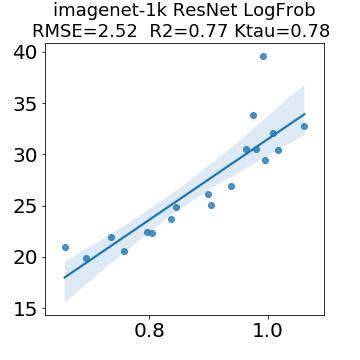
\includegraphics[width=3.7cm]{img/omsr_imagenet_1k_ResNet_lognorm}
        \label{fig:summary_regressions_A_01}
    }
    \subfigure[ imagenet-1k--ResNet, $\langle\log\Vert\cdot\Vert_{\infty}\rangle$ ]{
        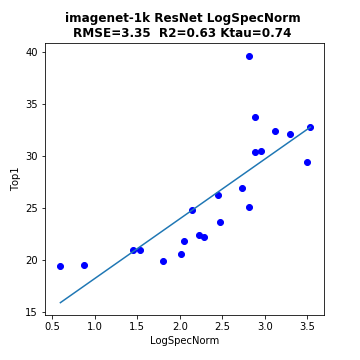
\includegraphics[width=3.7cm]{img/omsr_imagenet_1k_ResNet_spectralnormlog}
        \label{fig:summary_regressions_A_02}
    }
    \subfigure[ imagenet-1k--ResNet, $\hat{\alpha}$ ]{
        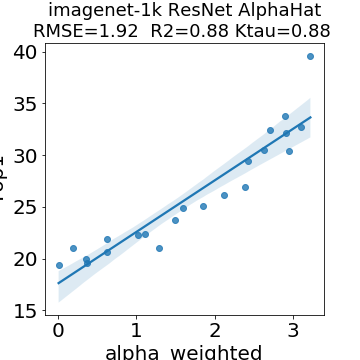
\includegraphics[width=3.7cm]{img/omsr_imagenet_1k_ResNet_alpha_weighted}
        \label{fig:summary_regressions_A_03}
    }
    \subfigure[ imagenet-1k--ResNet, $\langle\log\Vert\cdot\Vert^{\alpha}_{\alpha}\rangle$ ]{
        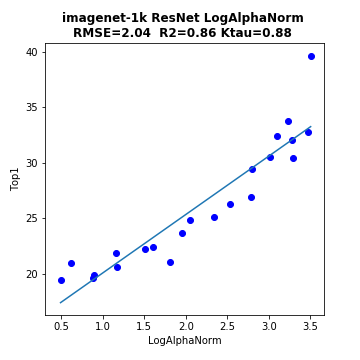
\includegraphics[width=3.7cm]{img/omsr_imagenet_1k_ResNet_logpnorm}
        \label{fig:summary_regressions_A_04}
    }
    \subfigure[ imagenet-1k--EfficientNet, $\langle\log\Vert\cdot\Vert_{F}\rangle$ ]{
        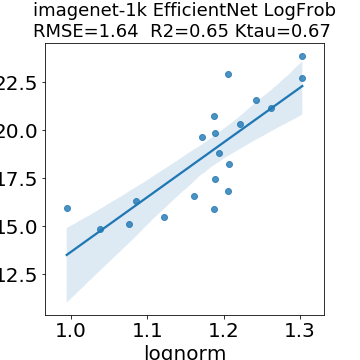
\includegraphics[width=3.7cm]{img/omsr_imagenet_1k_EfficientNet_lognorm}
        \label{fig:summary_regressions_A_05}
    }
    \subfigure[ imagenet-1k--EfficientNet, $\langle\log\Vert\cdot\Vert_{\infty}\rangle$ ]{
        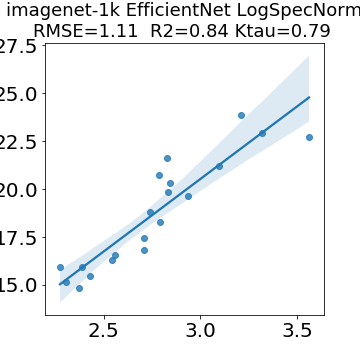
\includegraphics[width=3.7cm]{img/omsr_imagenet_1k_EfficientNet_spectralnormlog}
        \label{fig:summary_regressions_A_06}
    }
    \subfigure[ imagenet-1k--EfficientNet, $\hat{\alpha}$ ]{
        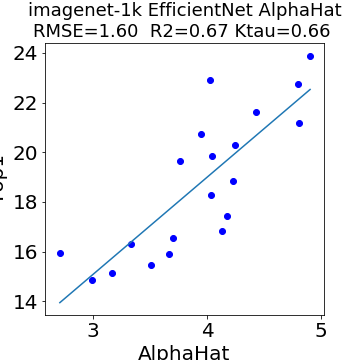
\includegraphics[width=3.7cm]{img/omsr_imagenet_1k_EfficientNet_alpha_weighted}
        \label{fig:summary_regressions_A_07}
    }
    \subfigure[ imagenet-1k--EfficientNet, $\langle\log\Vert\cdot\Vert^{\alpha}_{\alpha}\rangle$ ]{
        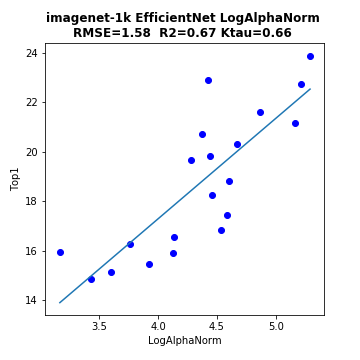
\includegraphics[width=3.7cm]{img/omsr_imagenet_1k_EfficientNet_logpnorm}
        \label{fig:summary_regressions_A_08}
    }
    \subfigure[ imagenet-1k--PreResNet, $\langle\log\Vert\cdot\Vert_{F}\rangle$ ]{
        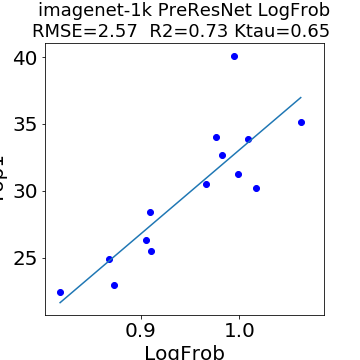
\includegraphics[width=3.7cm]{img/omsr_imagenet_1k_PreResNet_lognorm}
        \label{fig:summary_regressions_A_09}
    }
    \subfigure[ imagenet-1k--PreResNet, $\langle\log\Vert\cdot\Vert_{\infty}\rangle$ ]{
        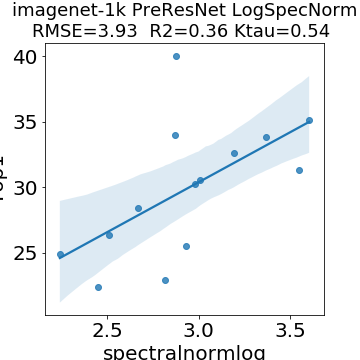
\includegraphics[width=3.7cm]{img/omsr_imagenet_1k_PreResNet_spectralnormlog}
        \label{fig:summary_regressions_A_10}
    }
    \subfigure[ imagenet-1k--PreResNet, $\hat{\alpha}$ ]{
        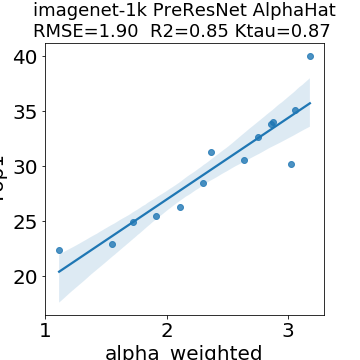
\includegraphics[width=3.7cm]{img/omsr_imagenet_1k_PreResNet_alpha_weighted}
        \label{fig:summary_regressions_A_11}
    }
    \subfigure[ imagenet-1k--PreResNet, $\langle\log\Vert\cdot\Vert^{\alpha}_{\alpha}\rangle$ ]{
        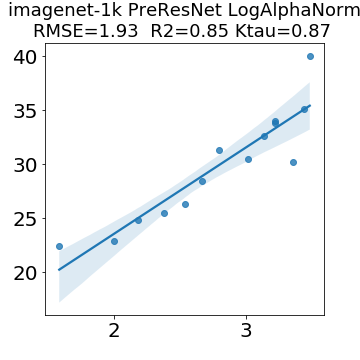
\includegraphics[width=3.7cm]{img/omsr_imagenet_1k_PreResNet_logpnorm}
        \label{fig:summary_regressions_A_12}
    }
    \caption{Regression plots for model-dataset pairs, based on data from Table~\ref{table:MSEresults}, Table~\ref{table:R2results}, and Table~\ref{table:KTresults}.
             Each row corresponds to a different dataset-model pair:
             imagenet-1k--ResNet; 
             imagenet-1k--EfficientNet; 
             and 
             imagenet-1k--PreResNet; 
             repsectively.
             Each column corresponds to a different metric:
             $\langle\log\Vert\cdot\Vert_{F}\rangle$; 
             $\langle\log\Vert\cdot\Vert_{\infty}\rangle$; 
             $\hat{\alpha}$; 
             and
             $\langle\log\Vert\cdot\Vert^{\alpha}_{\alpha}\rangle$;
             repsectively.
            }
    \label{fig:summary_regressions_A}
\end{figure}


 
\begin{figure}[t]
    \centering
    \subfigure[ imagenet-1k--ShuffleNet, $\langle\log\Vert\cdot\Vert_{F}\rangle$ ]{
        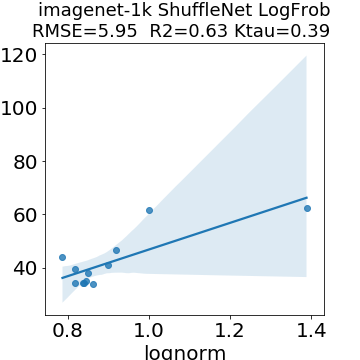
\includegraphics[width=3.7cm]{img/omsr_imagenet_1k_ShuffleNet_lognorm}
        \label{fig:summary_regressions_B_01}
    }
    \subfigure[ imagenet-1k--ShuffleNet, $\langle\log\Vert\cdot\Vert_{\infty}\rangle$ ]{
        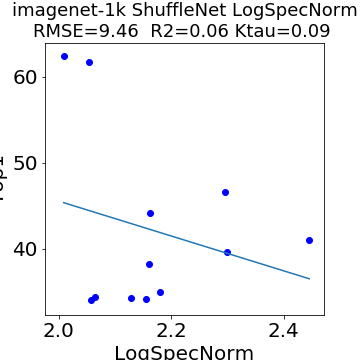
\includegraphics[width=3.7cm]{img/omsr_imagenet_1k_ShuffleNet_spectralnormlog}
        \label{fig:summary_regressions_B_02}
    }
    \subfigure[ imagenet-1k--ShuffleNet, $\hat{\alpha}$ ]{
        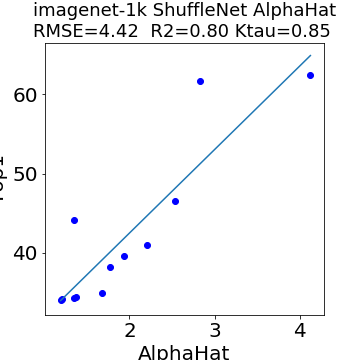
\includegraphics[width=3.7cm]{img/omsr_imagenet_1k_ShuffleNet_alpha_weighted}
        \label{fig:summary_regressions_B_03}
    }
    \subfigure[ imagenet-1k--ShuffleNet, $\langle\log\Vert\cdot\Vert^{\alpha}_{\alpha}\rangle$ ]{
        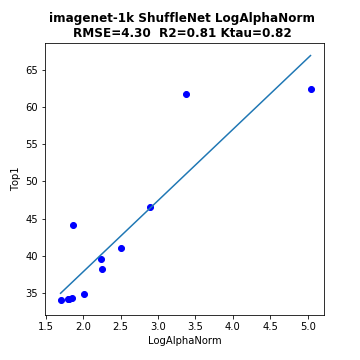
\includegraphics[width=3.7cm]{img/omsr_imagenet_1k_ShuffleNet_logpnorm}
        \label{fig:summary_regressions_B_04}
    }
    \subfigure[ imagenet-1k--VGG, $\langle\log\Vert\cdot\Vert_{F}\rangle$ ]{
        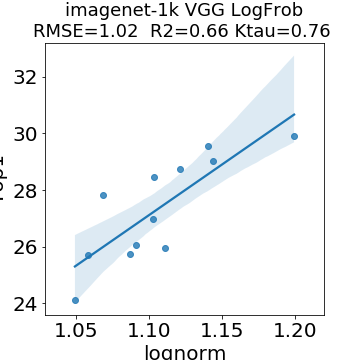
\includegraphics[width=3.7cm]{img/omsr_imagenet_1k_VGG_lognorm}
        \label{fig:summary_regressions_B_05}
    }
    \subfigure[ imagenet-1k--VGG, $\langle\log\Vert\cdot\Vert_{\infty}\rangle$ ]{
        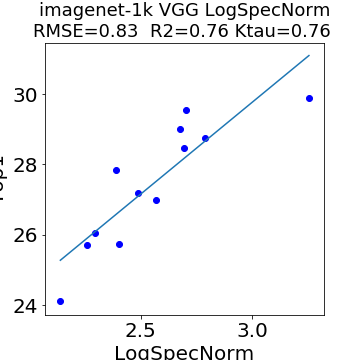
\includegraphics[width=3.7cm]{img/omsr_imagenet_1k_VGG_spectralnormlog}
        \label{fig:summary_regressions_B_06}
    }
    \subfigure[ imagenet-1k--VGG, $\hat{\alpha}$ ]{
        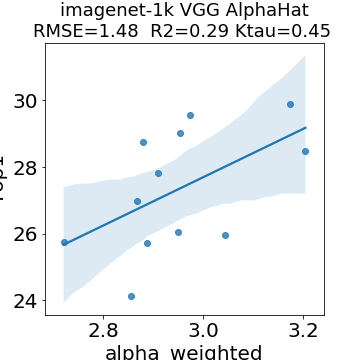
\includegraphics[width=3.7cm]{img/omsr_imagenet_1k_VGG_alpha_weighted}
        \label{fig:summary_regressions_B_07}
    }
    \subfigure[ imagenet-1k--VGG, $\langle\log\Vert\cdot\Vert^{\alpha}_{\alpha}\rangle$ ]{
        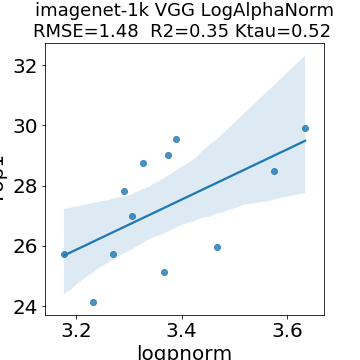
\includegraphics[width=3.7cm]{img/omsr_imagenet_1k_VGG_logpnorm}
        \label{fig:summary_regressions_B_08}
    }
    \subfigure[ imagenet-1k--DLA, $\langle\log\Vert\cdot\Vert_{F}\rangle$ ]{
        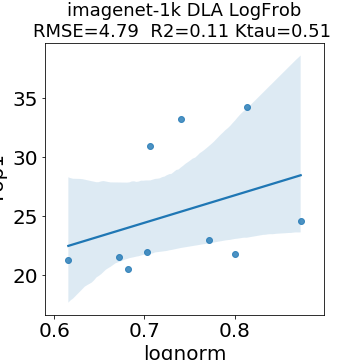
\includegraphics[width=3.7cm]{img/omsr_imagenet_1k_DLA_lognorm}
        \label{fig:summary_regressions_B_09}
    }
    \subfigure[ imagenet-1k--DLA, $\langle\log\Vert\cdot\Vert_{\infty}\rangle$ ]{
        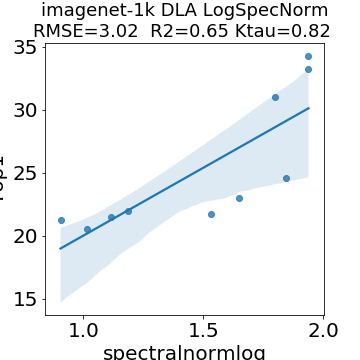
\includegraphics[width=3.7cm]{img/omsr_imagenet_1k_DLA_spectralnormlog}
        \label{fig:summary_regressions_B_10}
    }
    \subfigure[ imagenet-1k--DLA, $\hat{\alpha}$ ]{
        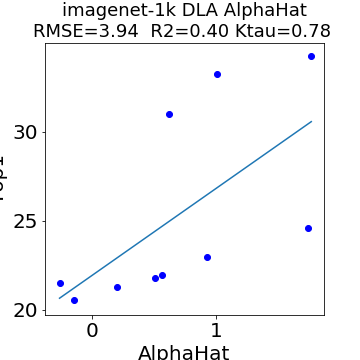
\includegraphics[width=3.7cm]{img/omsr_imagenet_1k_DLA_alpha_weighted}
        \label{fig:summary_regressions_B_11}
    }
    \subfigure[ imagenet-1k--DLA, $\langle\log\Vert\cdot\Vert^{\alpha}_{\alpha}\rangle$ ]{
        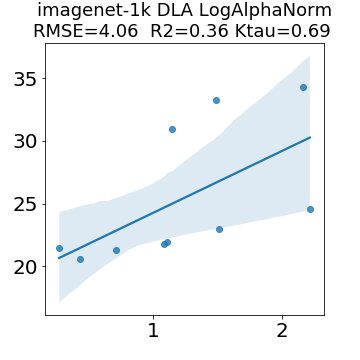
\includegraphics[width=3.7cm]{img/omsr_imagenet_1k_DLA_logpnorm}
        \label{fig:summary_regressions_B_12}
    }
    \caption{Regression plots for model-dataset pairs, based on data from Table~\ref{table:RMSEresults}, Table~\ref{table:R2results}, and Table~\ref{table:Ktauresults}.
             Each row corresponds to a different dataset-model pair:
             imagenet-1k--ShuffleNet;
             imagenet-1k--VGG;
             and
             imagenet-1k--DLA;
             repsectively.
             Each column corresponds to a different metric:
             $\langle\log\Vert\cdot\Vert_{F}\rangle$; 
             $\langle\log\Vert\cdot\Vert_{\infty}\rangle$; 
             $\hat{\alpha}$; 
             and
             $\langle\log\Vert\cdot\Vert^{\alpha}_{\alpha}\rangle$;
             repsectively.
            }
    \label{fig:summary_regressions_B}
\end{figure}


 
\begin{figure}[t]
    \centering
    \subfigure[ imagenet-1k--HRNet, $\langle\log\Vert\cdot\Vert_{F}\rangle$ ]{
        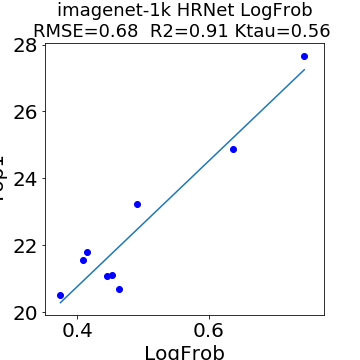
\includegraphics[width=3.7cm]{img/omsr_imagenet_1k_HRNet_lognorm}
        \label{fig:summary_regressions_C_01}
    }
    \subfigure[ imagenet-1k--HRNet, $\langle\log\Vert\cdot\Vert_{\infty}\rangle$ ]{
        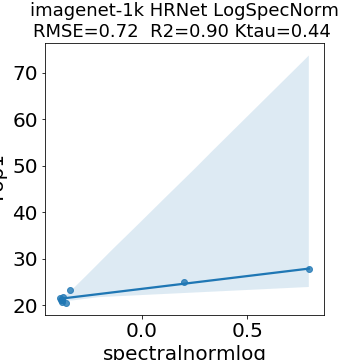
\includegraphics[width=3.7cm]{img/omsr_imagenet_1k_HRNet_spectralnormlog}
        \label{fig:summary_regressions_C_02}
    }
    \subfigure[ imagenet-1k--HRNet, $\hat{\alpha}$ ]{
        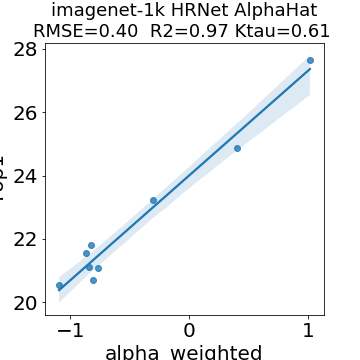
\includegraphics[width=3.7cm]{img/omsr_imagenet_1k_HRNet_alpha_weighted}
        \label{fig:summary_regressions_C_03}
    }
    \subfigure[ imagenet-1k--HRNet, $\langle\log\Vert\cdot\Vert^{\alpha}_{\alpha}\rangle$ ]{
        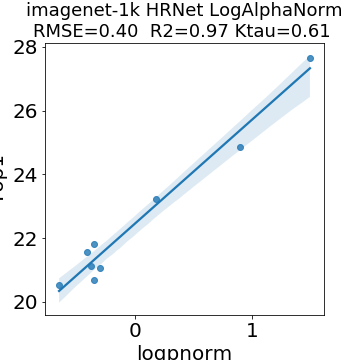
\includegraphics[width=3.7cm]{img/omsr_imagenet_1k_HRNet_logpnorm}
        \label{fig:summary_regressions_C_04}
    }
    \subfigure[ imagenet-1k--DRN-C, $\langle\log\Vert\cdot\Vert_{F}\rangle$ ]{
        \includegraphics[width=3.7cm]{img/omsr_imagenet_1k_DRN_C_lognorm}
        \label{fig:summary_regressions_C_05}
    }
    \subfigure[ imagenet-1k--DRN-C, $\langle\log\Vert\cdot\Vert_{\infty}\rangle$ ]{
        \includegraphics[width=3.7cm]{img/omsr_imagenet_1k_DRN_C_spectralnormlog}
        \label{fig:summary_regressions_C_06}
    }
    \subfigure[ imagenet-1k--DRN-C, $\hat{\alpha}$ ]{
        \includegraphics[width=3.7cm]{img/omsr_imagenet_1k_DRN_C_alpha_weighted}
        \label{fig:summary_regressions_C_07}
    }
    \subfigure[ imagenet-1k--DRN-C, $\langle\log\Vert\cdot\Vert^{\alpha}_{\alpha}\rangle$ ]{
        \includegraphics[width=3.7cm]{img/omsr_imagenet_1k_DRN_C_logpnorm}
        \label{fig:summary_regressions_C_08}
    }
    \subfigure[ imagenet-1k--SqueezeNext, $\langle\log\Vert\cdot\Vert_{F}\rangle$ ]{
        \includegraphics[width=3.7cm]{img/omsr_imagenet_1k_SqueezeNext_lognorm}
        \label{fig:summary_regressions_C_09}
    }
    \subfigure[ imagenet-1k--SqueezeNext, $\langle\log\Vert\cdot\Vert_{\infty}\rangle$ ]{
        \includegraphics[width=3.7cm]{img/omsr_imagenet_1k_SqueezeNext_spectralnormlog}
        \label{fig:summary_regressions_C_10}
    }
    \subfigure[ imagenet-1k--SqueezeNext, $\hat{\alpha}$ ]{
        \includegraphics[width=3.7cm]{img/omsr_imagenet_1k_SqueezeNext_alpha_weighted}
        \label{fig:summary_regressions_C_11}
    }
    \subfigure[ imagenet-1k--SqueezeNext, $\langle\log\Vert\cdot\Vert^{\alpha}_{\alpha}\rangle$ ]{
        \includegraphics[width=3.7cm]{img/omsr_imagenet_1k_SqueezeNext_logpnorm}
        \label{fig:summary_regressions_C_12}
    }
    \caption{Regression plots for model-dataset pairs, based on data from Table~\ref{table:MSEresults}, Table~\ref{table:R2results}, and Table~\ref{table:KTresults}.
             Each row corresponds to a different dataset-model pair:
             imagenet-1k--HRNet;
             imagenet-1k--DRN-C;
             and
             imagenet-1k--SqueezeNext;
             repsectively.
             Each column corresponds to a different metric:
             $\langle\log\Vert\cdot\Vert_{F}\rangle$; 
             $\langle\log\Vert\cdot\Vert_{\infty}\rangle$; 
             $\hat{\alpha}$; 
             and
             $\langle\log\Vert\cdot\Vert^{\alpha}_{\alpha}\rangle$;
             repsectively.
            }
    \label{fig:summary_regressions_C}
\end{figure}


 
\begin{figure}[t]
    \centering
    \subfigure[ imagenet-1k--ESPNetv2, $\langle\log\Vert\cdot\Vert_{F}\rangle$ ]{
        \includegraphics[width=3.7cm]{img/omsr_imagenet_1k_ESPNetv2_lognorm}
        \label{fig:summary_regressions_D_01}
    }
    \subfigure[ imagenet-1k--ESPNetv2, $\langle\log\Vert\cdot\Vert_{\infty}\rangle$ ]{
        \includegraphics[width=3.7cm]{img/omsr_imagenet_1k_ESPNetv2_spectralnormlog}
        \label{fig:summary_regressions_D_02}
    }
    \subfigure[ imagenet-1k--ESPNetv2, $\hat{\alpha}$ ]{
        \includegraphics[width=3.7cm]{img/omsr_imagenet_1k_ESPNetv2_alpha_weighted}
        \label{fig:summary_regressions_D_03}
    }
    \subfigure[ imagenet-1k--ESPNetv2, $\langle\log\Vert\cdot\Vert^{\alpha}_{\alpha}\rangle$ ]{
        \includegraphics[width=3.7cm]{img/omsr_imagenet_1k_ESPNetv2_logpnorm}
        \label{fig:summary_regressions_D_04}
    }
    \subfigure[ imagenet-1k--SqueezeNet, $\langle\log\Vert\cdot\Vert_{F}\rangle$ ]{
        \includegraphics[width=3.7cm]{img/omsr_imagenet_1k_SqueezeNet_lognorm}
        \label{fig:summary_regressions_D_05}
    }
    \subfigure[ imagenet-1k--SqueezeNet, $\langle\log\Vert\cdot\Vert_{\infty}\rangle$ ]{
        \includegraphics[width=3.7cm]{img/omsr_imagenet_1k_SqueezeNet_spectralnormlog}
        \label{fig:summary_regressions_D_06}
    }
    \subfigure[ imagenet-1k--SqueezeNet, $\hat{\alpha}$ ]{
        \includegraphics[width=3.7cm]{img/omsr_imagenet_1k_SqueezeNet_alpha_weighted}
        \label{fig:summary_regressions_D_07}
    }
    \subfigure[ imagenet-1k--SqueezeNet, $\langle\log\Vert\cdot\Vert^{\alpha}_{\alpha}\rangle$ ]{
        \includegraphics[width=3.7cm]{img/omsr_imagenet_1k_SqueezeNet_logpnorm}
        \label{fig:summary_regressions_D_08}
    }
    \subfigure[ imagenet-1k--ProxylessNAS, $\langle\log\Vert\cdot\Vert_{F}\rangle$ ]{
        \includegraphics[width=3.7cm]{img/omsr_imagenet_1k_ProxylessNAS_lognorm}
        \label{fig:summary_regressions_D_09}
    }
    \subfigure[ imagenet-1k--ProxylessNAS, $\langle\log\Vert\cdot\Vert_{\infty}\rangle$ ]{
        \includegraphics[width=3.7cm]{img/omsr_imagenet_1k_ProxylessNAS_spectralnormlog}
        \label{fig:summary_regressions_D_10}
    }
    \subfigure[ imagenet-1k--ProxylessNAS, $\hat{\alpha}$ ]{
        \includegraphics[width=3.7cm]{img/omsr_imagenet_1k_ProxylessNAS_alpha_weighted}
        \label{fig:summary_regressions_D_11}
    }
    \subfigure[ imagenet-1k--ProxylessNAS, $\langle\log\Vert\cdot\Vert^{\alpha}_{\alpha}\rangle$ ]{
        \includegraphics[width=3.7cm]{img/omsr_imagenet_1k_ProxylessNAS_logpnorm}
        \label{fig:summary_regressions_D_12}
    }
    \caption{Regression plots for model-dataset pairs, based on data from Table~\ref{table:MSEresults}, Table~\ref{table:R2results}, and Table~\ref{table:KTresults}.
             Each row corresponds to a different dataset-model pair:
             imagenet-1k--ESPNetv2;
             imagenet-1k--SqueezeNet;
             and
             imagenet-1k--ProxylessNAS;
             repsectively.
             Each column corresponds to a different metric:
             $\langle\log\Vert\cdot\Vert_{F}\rangle$; 
             $\langle\log\Vert\cdot\Vert_{\infty}\rangle$; 
             $\hat{\alpha}$; 
             and
             $\langle\log\Vert\cdot\Vert^{\alpha}_{\alpha}\rangle$;
             repsectively.
            }
    \label{fig:summary_regressions_D}
\end{figure}


 
\begin{figure}[t]
    \centering
    \subfigure[ imagenet-1k--IGCV3, $\langle\log\Vert\cdot\Vert_{F}\rangle$ ]{
        \includegraphics[width=3.7cm]{img/omsr_imagenet_1k_IGCV3_lognorm}
        \label{fig:summary_regressions_E_01}
    }
    \subfigure[ imagenet-1k--IGCV3, $\langle\log\Vert\cdot\Vert_{\infty}\rangle$ ]{
        \includegraphics[width=3.7cm]{img/omsr_imagenet_1k_IGCV3_spectralnormlog}
        \label{fig:summary_regressions_E_02}
    }
    \subfigure[ imagenet-1k--IGCV3, $\hat{\alpha}$ ]{
        \includegraphics[width=3.7cm]{img/omsr_imagenet_1k_IGCV3_alpha_weighted}
        \label{fig:summary_regressions_E_03}
    }
    \subfigure[ imagenet-1k--IGCV3, $\langle\log\Vert\cdot\Vert^{\alpha}_{\alpha}\rangle$ ]{
        \includegraphics[width=3.7cm]{img/omsr_imagenet_1k_IGCV3_logpnorm}
        \label{fig:summary_regressions_E_04}
    }
    \subfigure[ cifar-10--ResNet, $\langle\log\Vert\cdot\Vert_{F}\rangle$ ]{
        \includegraphics[width=3.7cm]{img/omsr_cifar_10_ResNet_lognorm}
        \label{fig:summary_regressions_E_05}
    }
    \subfigure[ cifar-10--ResNet, $\langle\log\Vert\cdot\Vert_{\infty}\rangle$ ]{
        \includegraphics[width=3.7cm]{img/omsr_cifar_10_ResNet_spectralnormlog}
        \label{fig:summary_regressions_E_06}
    }
    \subfigure[ cifar-10--ResNet, $\hat{\alpha}$ ]{
        \includegraphics[width=3.7cm]{img/omsr_cifar_10_ResNet_alpha_weighted}
        \label{fig:summary_regressions_E_07}
    }
    \subfigure[ cifar-10--ResNet, $\langle\log\Vert\cdot\Vert^{\alpha}_{\alpha}\rangle$ ]{
        \includegraphics[width=3.7cm]{img/omsr_cifar_10_ResNet_logpnorm}
        \label{fig:summary_regressions_E_08}
    }
    \subfigure[ cifar-10--DIA-ResNet, $\langle\log\Vert\cdot\Vert_{F}\rangle$ ]{
        \includegraphics[width=3.7cm]{img/omsr_cifar_10_DIA_ResNet_lognorm}
        \label{fig:summary_regressions_E_09}
    }
    \subfigure[ cifar-10--DIA-ResNet, $\langle\log\Vert\cdot\Vert_{\infty}\rangle$ ]{
        \includegraphics[width=3.7cm]{img/omsr_cifar_10_DIA_ResNet_spectralnormlog}
        \label{fig:summary_regressions_E_10}
    }
    \subfigure[ cifar-10--DIA-ResNet, $\hat{\alpha}$ ]{
        \includegraphics[width=3.7cm]{img/omsr_cifar_10_DIA_ResNet_alpha_weighted}
        \label{fig:summary_regressions_E_11}
    }
    \subfigure[ cifar-10--DIA-ResNet, $\langle\log\Vert\cdot\Vert^{\alpha}_{\alpha}\rangle$ ]{
        \includegraphics[width=3.7cm]{img/omsr_cifar_10_DIA_ResNet_logpnorm}
        \label{fig:summary_regressions_E_12}
    }
    \caption{Regression plots for model-dataset pairs, based on data from Table~\ref{table:RMSEresults}, Table~\ref{table:R2results}, and Table~\ref{table:Ktauresults}.
             Each row corresponds to a different dataset-model pair:
             imagenet-1k--IGCV3;
             cifar-10--ResNet;
             and
             cifar-10--DIA-ResNet;
             repsectively.
             Each column corresponds to a different metric:
             $\langle\log\Vert\cdot\Vert_{F}\rangle$; 
             $\langle\log\Vert\cdot\Vert_{\infty}\rangle$; 
             $\hat{\alpha}$; 
             and
             $\langle\log\Vert\cdot\Vert^{\alpha}_{\alpha}\rangle$;
             repsectively.
            }
    \label{fig:summary_regressions_E}
\end{figure}


 
\begin{figure}[t]
    \centering
    \subfigure[ cifar-10--SENet, $\langle\log\Vert\cdot\Vert_{F}\rangle$ ]{
        \includegraphics[width=3.7cm]{img/omsr_cifar_10_SENet_lognorm}
        \label{fig:summary_regressions_F_01}
    }
    \subfigure[ cifar-10--SENet, $\langle\log\Vert\cdot\Vert_{\infty}\rangle$ ]{
        \includegraphics[width=3.7cm]{img/omsr_cifar_10_SENet_spectralnormlog}
        \label{fig:summary_regressions_F_02}
    }
    \subfigure[ cifar-10--SENet, $\hat{\alpha}$ ]{
        \includegraphics[width=3.7cm]{img/omsr_cifar_10_SENet_alpha_weighted}
        \label{fig:summary_regressions_F_03}
    }
    \subfigure[ cifar-10--SENet, $\langle\log\Vert\cdot\Vert^{\alpha}_{\alpha}\rangle$ ]{
        \includegraphics[width=3.7cm]{img/omsr_cifar_10_SENet_logpnorm}
        \label{fig:summary_regressions_F_04}
    }
    \subfigure[ cifar-100--ResNet, $\langle\log\Vert\cdot\Vert_{F}\rangle$ ]{
        \includegraphics[width=3.7cm]{img/omsr_cifar_100_ResNet_lognorm}
        \label{fig:summary_regressions_F_05}
    }
    \subfigure[ cifar-100--ResNet, $\langle\log\Vert\cdot\Vert_{\infty}\rangle$ ]{
        \includegraphics[width=3.7cm]{img/omsr_cifar_100_ResNet_spectralnormlog}
        \label{fig:summary_regressions_F_06}
    }
    \subfigure[ cifar-100--ResNet, $\hat{\alpha}$ ]{
        \includegraphics[width=3.7cm]{img/omsr_cifar_100_ResNet_alpha_weighted}
        \label{fig:summary_regressions_F_07}
    }
    \subfigure[ cifar-100--ResNet, $\langle\log\Vert\cdot\Vert^{\alpha}_{\alpha}\rangle$ ]{
        \includegraphics[width=3.7cm]{img/omsr_cifar_100_ResNet_logpnorm}
        \label{fig:summary_regressions_F_08}
    }
    \subfigure[ cifar-100--DIA-ResNet, $\langle\log\Vert\cdot\Vert_{F}\rangle$ ]{
        \includegraphics[width=3.7cm]{img/omsr_cifar_100_DIA_ResNet_lognorm}
        \label{fig:summary_regressions_F_09}
    }
    \subfigure[ cifar-100--DIA-ResNet, $\langle\log\Vert\cdot\Vert_{\infty}\rangle$ ]{
        \includegraphics[width=3.7cm]{img/omsr_cifar_100_DIA_ResNet_spectralnormlog}
        \label{fig:summary_regressions_F_10}
    }
    \subfigure[ cifar-100--DIA-ResNet, $\hat{\alpha}$ ]{
        \includegraphics[width=3.7cm]{img/omsr_cifar_100_DIA_ResNet_alpha_weighted}
        \label{fig:summary_regressions_F_11}
    }
    \subfigure[ cifar-100--DIA-ResNet, $\langle\log\Vert\cdot\Vert^{\alpha}_{\alpha}\rangle$ ]{
        \includegraphics[width=3.7cm]{img/omsr_cifar_100_DIA_ResNet_logpnorm}
        \label{fig:summary_regressions_F_12}
    }
    \caption{Regression plots for model-dataset pairs, based on data from Table~\ref{table:MSEresults}, Table~\ref{table:R2results}, and Table~\ref{table:KTresults}.
             Each row corresponds to a different dataset-model pair:
             cifar-10--SENet;
             cifar-100--ResNet;
             and
             cifar-100--DIA-ResNet;
             repsectively.
             Each column corresponds to a different metric:
             $\langle\log\Vert\cdot\Vert_{F}\rangle$; 
             $\langle\log\Vert\cdot\Vert_{\infty}\rangle$; 
             $\hat{\alpha}$; 
             and
             $\langle\log\Vert\cdot\Vert^{\alpha}_{\alpha}\rangle$;
             repsectively.
            }
    \label{fig:summary_regressions_F}
\end{figure}


 
\begin{figure}[t]
    \centering
    \subfigure[ cifar-100--SENet, $\langle\log\Vert\cdot\Vert_{F}\rangle$ ]{
        \includegraphics[width=3.7cm]{img/omsr_cifar_100_SENet_lognorm}
        \label{fig:summary_regressions_G_01}
    }
    \subfigure[ cifar-100--SENet, $\langle\log\Vert\cdot\Vert_{\infty}\rangle$ ]{
        \includegraphics[width=3.7cm]{img/omsr_cifar_100_SENet_spectralnormlog}
        \label{fig:summary_regressions_G_02}
    }
    \subfigure[ cifar-100--SENet, $\hat{\alpha}$ ]{
        \includegraphics[width=3.7cm]{img/omsr_cifar_100_SENet_alpha_weighted}
        \label{fig:summary_regressions_G_03}
    }
    \subfigure[ cifar-100--SENet, $\langle\log\Vert\cdot\Vert^{\alpha}_{\alpha}\rangle$ ]{
        \includegraphics[width=3.7cm]{img/omsr_cifar_100_SENet_logpnorm}
        \label{fig:summary_regressions_G_04}
    }
    \subfigure[ cifar-100--WRN, $\langle\log\Vert\cdot\Vert_{F}\rangle$ ]{
        \includegraphics[width=3.7cm]{img/omsr_cifar_100_WRN_lognorm}
        \label{fig:summary_regressions_G_05}
    }
    \subfigure[ cifar-100--WRN, $\langle\log\Vert\cdot\Vert_{\infty}\rangle$ ]{
        \includegraphics[width=3.7cm]{img/omsr_cifar_100_WRN_spectralnormlog}
        \label{fig:summary_regressions_G_06}
    }
    \subfigure[ cifar-100--WRN, $\hat{\alpha}$ ]{
        \includegraphics[width=3.7cm]{img/omsr_cifar_100_WRN_alpha_weighted}
        \label{fig:summary_regressions_G_07}
    }
    \subfigure[ cifar-100--WRN, $\langle\log\Vert\cdot\Vert^{\alpha}_{\alpha}\rangle$ ]{
        \includegraphics[width=3.7cm]{img/omsr_cifar_100_WRN_logpnorm}
        \label{fig:summary_regressions_G_08}
    }
    \subfigure[ svhn--ResNet, $\langle\log\Vert\cdot\Vert_{F}\rangle$ ]{
        \includegraphics[width=3.7cm]{img/omsr_svhn_ResNet_lognorm}
        \label{fig:summary_regressions_G_09}
    }
    \subfigure[ svhn--ResNet, $\langle\log\Vert\cdot\Vert_{\infty}\rangle$ ]{
        \includegraphics[width=3.7cm]{img/omsr_svhn_ResNet_spectralnormlog}
        \label{fig:summary_regressions_G_10}
    }
    \subfigure[ svhn--ResNet, $\hat{\alpha}$ ]{
        \includegraphics[width=3.7cm]{img/omsr_svhn_ResNet_alpha_weighted}
        \label{fig:summary_regressions_G_11}
    }
    \subfigure[ svhn--ResNet, $\langle\log\Vert\cdot\Vert^{\alpha}_{\alpha}\rangle$ ]{
        \includegraphics[width=3.7cm]{img/omsr_svhn_ResNet_logpnorm}
        \label{fig:summary_regressions_G_12}
    }
    \caption{Regression plots for model-dataset pairs, based on data from Table~\ref{table:MSEresults}, Table~\ref{table:R2results}, and Table~\ref{table:KTresults}.
             Each row corresponds to a different dataset-model pair:
             cifar-100--SENet;
             cifar-100--WRN;
             and
             svhn--ResNet;
             repsectively.
             Each column corresponds to a different metric:
             $\langle\log\Vert\cdot\Vert_{F}\rangle$; 
             $\langle\log\Vert\cdot\Vert_{\infty}\rangle$; 
             $\hat{\alpha}$; 
             and
             $\langle\log\Vert\cdot\Vert^{\alpha}_{\alpha}\rangle$;
             repsectively.
            }
    \label{fig:summary_regressions_G}
\end{figure}


 
\begin{figure}[t]
    \centering
    \subfigure[ svhn--DIA-ResNet, $\langle\log\Vert\cdot\Vert_{F}\rangle$ ]{
        \includegraphics[width=3.7cm]{img/omsr_svhn_DIA_ResNet_lognorm}
        \label{fig:summary_regressions_H_01}
    }
    \subfigure[ svhn--DIA-ResNet, $\langle\log\Vert\cdot\Vert_{\infty}\rangle$ ]{
        \includegraphics[width=3.7cm]{img/omsr_svhn_DIA_ResNet_spectralnormlog}
        \label{fig:summary_regressions_H_02}
    }
    \subfigure[ svhn--DIA-ResNet, $\hat{\alpha}$ ]{
        \includegraphics[width=3.7cm]{img/omsr_svhn_DIA_ResNet_alpha_weighted}
        \label{fig:summary_regressions_H_03}
    }
    \subfigure[ svhn--DIA-ResNet, $\langle\log\Vert\cdot\Vert^{\alpha}_{\alpha}\rangle$ ]{
        \includegraphics[width=3.7cm]{img/omsr_svhn_DIA_ResNet_logpnorm}
        \label{fig:summary_regressions_H_04}
    }
    \subfigure[ svhn--SENet, $\langle\log\Vert\cdot\Vert_{F}\rangle$ ]{
        \includegraphics[width=3.7cm]{img/omsr_svhn_SENet_lognorm}
        \label{fig:summary_regressions_H_05}
    }
    \subfigure[ svhn--SENet, $\langle\log\Vert\cdot\Vert_{\infty}\rangle$ ]{
        \includegraphics[width=3.7cm]{img/omsr_svhn_SENet_spectralnormlog}
        \label{fig:summary_regressions_H_06}
    }
    \subfigure[ svhn--SENet, $\hat{\alpha}$ ]{
        \includegraphics[width=3.7cm]{img/omsr_svhn_SENet_alpha_weighted}
        \label{fig:summary_regressions_H_07}
    }
    \subfigure[ svhn--SENet, $\langle\log\Vert\cdot\Vert^{\alpha}_{\alpha}\rangle$ ]{
        \includegraphics[width=3.7cm]{img/omsr_svhn_SENet_logpnorm}
        \label{fig:summary_regressions_H_08}
    }
    \subfigure[ svhn--WRN, $\langle\log\Vert\cdot\Vert_{F}\rangle$ ]{
        \includegraphics[width=3.7cm]{img/omsr_svhn_WRN_lognorm}
        \label{fig:summary_regressions_H_09}
    }
    \subfigure[ svhn--WRN, $\langle\log\Vert\cdot\Vert_{\infty}\rangle$ ]{
        \includegraphics[width=3.7cm]{img/omsr_svhn_WRN_spectralnormlog}
        \label{fig:summary_regressions_H_10}
    }
    \subfigure[ svhn--WRN, $\hat{\alpha}$ ]{
        \includegraphics[width=3.7cm]{img/omsr_svhn_WRN_alpha_weighted}
        \label{fig:summary_regressions_H_11}
    }
    \subfigure[ svhn--WRN, $\langle\log\Vert\cdot\Vert^{\alpha}_{\alpha}\rangle$ ]{
        \includegraphics[width=3.7cm]{img/omsr_svhn_WRN_logpnorm}
        \label{fig:summary_regressions_H_12}
    }
    \caption{Regression plots for model-dataset pairs, based on data from Table~\ref{table:RMSEresults}, Table~\ref{table:R2results}, and Table~\ref{table:Ktauresults}.
             Each row corresponds to a different dataset-model pair:
             svhn--DIA-ResNet;
             svhn--SENet;
             and
             svhn--WRN;
             repsectively.
             Each column corresponds to a different metric:
             $\langle\log\Vert\cdot\Vert_{F}\rangle$; 
             $\langle\log\Vert\cdot\Vert_{\infty}\rangle$; 
             $\hat{\alpha}$; 
             and
             $\langle\log\Vert\cdot\Vert^{\alpha}_{\alpha}\rangle$;
             repsectively.
            }
    \label{fig:summary_regressions_H}
\end{figure}


 
\begin{figure}[t]
    \centering
    \subfigure[ svhn--ResNeXt, $\langle\log\Vert\cdot\Vert_{F}\rangle$ ]{
        \includegraphics[width=3.7cm]{img/omsr_svhn_ResNeXt_lognorm}
        \label{fig:summary_regressions_I_01}
    }
    \subfigure[ svhn--ResNeXt, $\langle\log\Vert\cdot\Vert_{\infty}\rangle$ ]{
        \includegraphics[width=3.7cm]{img/omsr_svhn_ResNeXt_spectralnormlog}
        \label{fig:summary_regressions_I_02}
    }
    \subfigure[ svhn--ResNeXt, $\hat{\alpha}$ ]{
        \includegraphics[width=3.7cm]{img/omsr_svhn_ResNeXt_alpha_weighted}
        \label{fig:summary_regressions_I_03}
    }
    \subfigure[ svhn--ResNeXt, $\langle\log\Vert\cdot\Vert^{\alpha}_{\alpha}\rangle$ ]{
        \includegraphics[width=3.7cm]{img/omsr_svhn_ResNeXt_logpnorm}
        \label{fig:summary_regressions_I_04}
    }
    \subfigure[ cub-200-2011--ResNet, $\langle\log\Vert\cdot\Vert_{F}\rangle$ ]{
        \includegraphics[width=3.7cm]{img/omsr_cub_200_2011_ResNet_lognorm}
        \label{fig:summary_regressions_I_05}
    }
    \subfigure[ cub-200-2011--ResNet, $\langle\log\Vert\cdot\Vert_{\infty}\rangle$ ]{
        \includegraphics[width=3.7cm]{img/omsr_cub_200_2011_ResNet_spectralnormlog}
        \label{fig:summary_regressions_I_06}
    }
    \subfigure[ cub-200-2011--ResNet, $\hat{\alpha}$ ]{
        \includegraphics[width=3.7cm]{img/omsr_cub_200_2011_ResNet_alpha_weighted}
        \label{fig:summary_regressions_I_07}
    }
    \subfigure[ cub-200-2011--ResNet, $\langle\log\Vert\cdot\Vert^{\alpha}_{\alpha}\rangle$ ]{
        \includegraphics[width=3.7cm]{img/omsr_cub_200_2011_ResNet_logpnorm}
        \label{fig:summary_regressions_I_08}
    }
    \subfigure[ cub-200-2011--SENet, $\langle\log\Vert\cdot\Vert_{F}\rangle$ ]{
        \includegraphics[width=3.7cm]{img/omsr_cub_200_2011_SENet_lognorm}
        \label{fig:summary_regressions_I_09}
    }
    \subfigure[ cub-200-2011--SENet, $\langle\log\Vert\cdot\Vert_{\infty}\rangle$ ]{
        \includegraphics[width=3.7cm]{img/omsr_cub_200_2011_SENet_spectralnormlog}
        \label{fig:summary_regressions_I_10}
    }
    \subfigure[ cub-200-2011--SENet, $\hat{\alpha}$ ]{
        \includegraphics[width=3.7cm]{img/omsr_cub_200_2011_SENet_alpha_weighted}
        \label{fig:summary_regressions_I_11}
    }
    \subfigure[ cub-200-2011--SENet, $\langle\log\Vert\cdot\Vert^{\alpha}_{\alpha}\rangle$ ]{
        \includegraphics[width=3.7cm]{img/omsr_cub_200_2011_SENet_logpnorm}
        \label{fig:summary_regressions_I_12}
    }
    \caption{Regression plots for model-dataset pairs, based on data from Table~\ref{table:RMSEresults}, Table~\ref{table:R2results}, and Table~\ref{table:Ktauresults}.
             Each row corresponds to a different dataset-model pair:
             svhn--ResNeXt;
             cub-200-2011--ResNet;
             and
             cub-200-2011--SENet;
             repsectively.
             Each column corresponds to a different metric:
             $\langle\log\Vert\cdot\Vert_{F}\rangle$; 
             $\langle\log\Vert\cdot\Vert_{\infty}\rangle$; 
             $\hat{\alpha}$; 
             and
             $\langle\log\Vert\cdot\Vert^{\alpha}_{\alpha}\rangle$;
             repsectively.
            }
    \label{fig:summary_regressions_I}
\end{figure}

 











\subsection{Supplementary Discussion: Additional Details on HT-SR Theory}

The original work on HT-SR Theory~\cite{MM18_TR,MM19_HTSR_ICML,MM20_SDM} considered DNNs including AlexNet and InceptionV3 (as well as DenseNet, ResNet, and VGG), and it showed that for nearly every $\mathbf{W}$, the (bulk and tail) of the ESDs can be fit to a truncated PL and the PL exponents $\alpha$ nearly all lie within the range $\alpha\in(1.5,5)$.
Our meta-analysis, the main results of which are summarized in this paper, has shown that these results are ubiquitous.
For example, 
upon examining nearly 10,000 layer weight matrices $\mathbf{W}_{l,i}$ across hundreds of different modern pre-trained DNN architectures, the ESD of nearly every $\mathbf{W}$ layer matrix can be fit to a truncated PL:
$70-80\%$ of the time, the fitted PL exponent $\alpha$ lies in the range $\alpha\in(2,4)$; and  
$10-20\%$ of the time, the fitted PL exponent $\alpha$ lies in the range $\alpha< 2$.  
Of course, there are exceptions: in any real DNN, the fitted $\alpha$ may range anywhere from $\sim 1.5$ to $10$ or higher (and, of course, larger values of $\alpha$ may indicate that the PL is not a good model for the data).  
Still, overall, in nearly all large, pre-trained DNNs, the correlations in the  weight matrices exhibit a remarkable Universality, being both Heavy Tailed, and having small---but not too small---PL exponents. 

